\documentclass[11pt]{article}
\usepackage[utf8]{inputenc}
\usepackage[spanish]{babel}
\decimalpoint
\usepackage{amsmath}
\usepackage{amsthm}
\usepackage{amssymb}
\usepackage{graphicx}
\usepackage[margin=0.8in]{geometry}
\usepackage{fancyhdr}
\usepackage[inline]{enumitem}
\usepackage{float}
\usepackage{cancel}
\usepackage{bigints}
\usepackage{listings}
\usepackage{xcolor}
\usepackage{listingsutf8}
\usepackage{algpseudocode}
\usepackage{algorithm}
\usepackage{apacite}
\usepackage{tcolorbox}
\usepackage{multicol}
\usepackage{tipa}
\usepackage{caption} 
\pagestyle{fancy}
\usepackage{hyperref}
\usepackage{mathtools}% http://ctan.org/pkg/mathtools
\hypersetup{
    colorlinks,
    citecolor=black,
    filecolor=black,
    linkcolor=black,
    urlcolor=black
}
\newcommand{\xvdash}[1]{%
	\vdash^{\mkern-10mu\scriptscriptstyle\rule[-.9ex]{0pt}{0pt}#1}%
}
\setlength{\headheight}{15pt} 
\lhead{Programa 1.- ECA regla 30}
\rhead{\thepage}
\lfoot{ESCOM-IPN}
\renewcommand{\footrulewidth}{0.5pt}
\setlength{\parskip}{0.5em}
\newcommand{\ve}[1]{\overrightarrow{#1}}
\newcommand{\abs}[1]{\left\lvert #1 \right\lvert}
\newcommand{\blank}{\text{\textcrb}}
\date{\today}
\title{ECA regla 30}
\author{Sanchez Mendez Edmundo Josue}

\lstdefinestyle{customc}{
	belowcaptionskip=1\baselineskip,
	breaklines=true,
	frame=L,
	xleftmargin=\parindent,
	language=C++,
	showstringspaces=false,
	basicstyle=\ttfamily,
	keywordstyle=\bfseries\color{green!40!black},
	commentstyle=\itshape\color{purple!40!black},
	identifierstyle=\color{blue},
	numbers=left,
	stringstyle=\color{orange},
}

\lstset{escapechar=@,style=customc,tabsize=3,language=C++}

\bibliographystyle{apacite}
\begin{document}
		\begin{titlepage}
			\begin{center}
				
				% Upper part of the page. The '~' is needed because \\
				% only works if a paragraph has started.
				
				\noindent
				\begin{minipage}{0.5\textwidth}
					\begin{flushleft} \large
						
\includegraphics[width=0.5\textwidth]{resources/ipn.png}
					\end{flushleft}
				\end{minipage}%
				\begin{minipage}{0.55\textwidth}
					\begin{flushright} \large
						
\includegraphics[width=0.5\textwidth]{resources/escom.png}
					\end{flushright}
				\end{minipage}
				
				\textsc{\LARGE Instituto Politécnico Nacional}\\[0.5cm]
				
				\textsc{\Large Escuela Superior de Cómputo}\\[1cm]
				
				% Title
				
				{ \huge Programa 1 - ECAs  \\[1cm] }
				
				{ \Large Unidad de aprendizaje: Computing Selected Topics} \\[1cm]
				
				{ \Large Grupo: 3CM19 } \\[1cm]
				
				\noindent
				\begin{minipage}{0.5\textwidth}
					\begin{flushleft} \large
						\emph{Alumno:} \\
						Sanchez Mendez Edmundo Josue
					\end{flushleft}
				\end{minipage}%
				\begin{minipage}{0.5\textwidth}
					\begin{flushright} \large
						\emph{Profesor:} \\
						Juarez Martinez Genaro
					\end{flushright}
				\end{minipage}
				
				\vfill
				% Bottom of the page
				{\large {\today}}
			\end{center}
		\end{titlepage}
	
	\titlepage
	\tableofcontents
	\newpage
	
	\begin{abstract}
		En este programa 1 se aborda la creación de un Autómata Celular Elemental o por sus siglas en ingles (ECA) tomando como regla a usar la regla 30(00011110$_2$), nuestro objetivo es poder generar dicho autómata con dicha regla y poder visualizar como este va evolucionando, permitiendo así poder generar un autómata como el siguiente ejemplo.
	\begin{figure}[H]
			\centering
			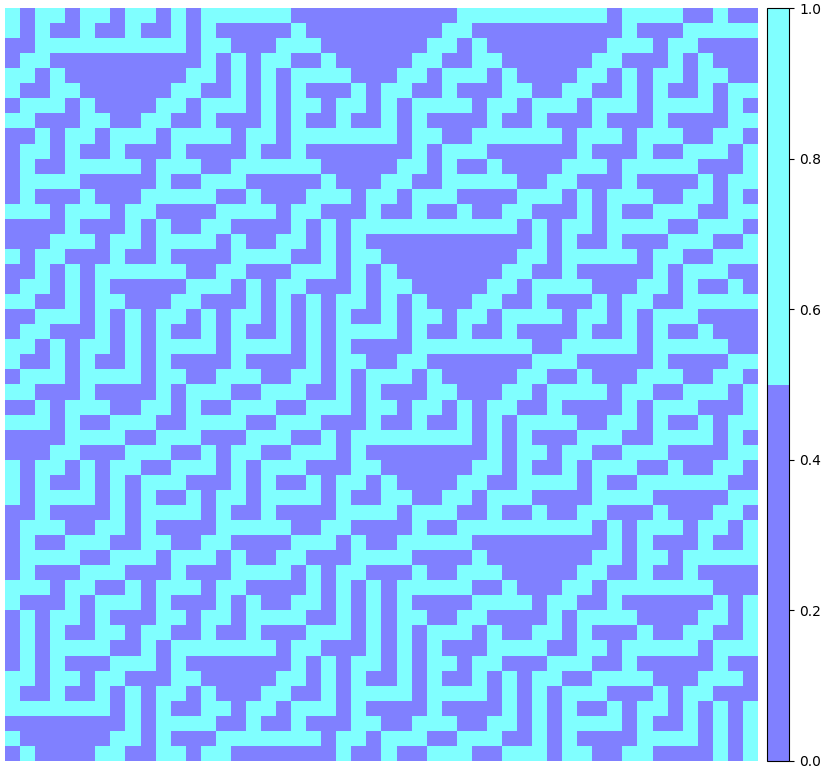
\includegraphics[scale=0.65]{resources/automata_50x50_r30.png}
			\caption{Autómata celular elemental aleatorio de 50 células evolucionado 50 veces}\label{fig:picture}
		\end{figure}
	\end{abstract}		
	
	\newpage
	
	\section{Introducción}
		Los autómatas celulares o por sus siglas (AC) surgen en la década de 1940 con John Von Neumann y fue  descrito en su libro $"$Theory of Self-reproducing Automata$"$, este tipo de autómatas son modelos matemáticos que valga la redundancia modelan sistemas dinámicos, los cuales evolucionan con el paso de tiempo, John Von Neumann tenia como objetivo modelar una máquina, que fuese capaz de auto replicarse, al intentar esto llego a un modelo matemático, el cual describe a dicha máquina con ciertas reglas sobre una red rectangular. Su nombre se debe a esta similitud con el crecimiento de las células.
	
	\section{Definición}
Como ya se mencionado anteriormente, un autómata celular es un modelo matemático para un sistema dinámico, este sistema evoluciona con el paso del tiempo. El autómata celular está compuesto por un conjunto células o celdas las cuales adquieren distintos valores o estados. Al ser este un sistema dinámico y al evolucionar a través del tiempo estos estados o valores que poseen las células son alterados de un instante a otro en un tiempo discreto, es decir, conocemos que valores toman nuestras células o celda en un cierto punto en el tiempo, en otras palabras es posible hacer una cuantización.
Siendo así, el conjunto de células evolucionan según la expresión matemática, la cual evolucionará según los estados de las células vecinas, a esto se le conoce como regla de transición local.

	
	\section{Elementos de un AC}
		\subsection{Un espacio rectangular}
		El autómata celular está definido ya sea en un espacio de dos dimensiones o bien en un espacio de n dimensiones, este es el espacio de evoluciones y cada una de las divisiones de este espacio es llamada célula.
		
		\subsection{Conjunto de estados}
		Los estados son finitos y cada elemento de la célula tomará un valor de este conjunto de estados. A cada vecindad diferente le corresponde un elemento del conjunto de estados.
 	
		\subsection{Configuración inicial o tiempo 0}
		Es la asignación inicial de un estado a cada una de las células del espacio.		
		
		\subsection{Función local o Función de transición local}
		Es la regla de evolución que determina el comportamiento del autómata celular. Esta regla esta conformada por una célula central y sus vecindades. También esta define como debe cambiar de estado cada una de las células dependiendo de los estados de las vecindades anteriores. Esta función puede ser representada como una función algebraica o como un conjunto de ecuaciones.
		
	
	\section{Tipos de límites o fronteras}
	Podemos hacer una representación visual de los autómatas celulares, y para que podamos entenderlo de mejor manera es necesario mencionar los límites y las fronteras, del espacio en el cual existe el autómata celular

		\subsection{Frontera abierta}
		Considera que todas las células fuera del espacio del autómata tienen un valor el cual es fijo.	
		
		\subsection{Frontera reflectora}
		Las células fuera del espacio del autómata toman los valores que están dentro como si se tratase de un espejo.

		\subsection{Frontera periódica o circular}
		Las células que están en los límites o en la frontera interaccionan con sus vecinos inmediatos y con las células que están en el extremo opuesto del arreglo, como si el plano estuviese doblado a manera de cilindro.
		
		\subsection{Sin frontera}
		La representación des autómata no tiene limites, en otras palabras es infinito.

	
	
	\section{Clasificación de los Autómatas Celulares}
	Stephen Wolfram comenzó a trabajar en autómatas celulares a mediados de 1981 después de considerar cómo los patrones complejos parecían formarse en la naturaleza en violación de la segunda ley de la termodinámica. Sus investigaciones fueron inicialmente impulsados por un interés en sistemas de modelado, como las redes neuronales. Tras ver la inesperada complejidad del comportamiento de estas reglas simples Wolfram llevó a sospechar que la complejidad en la naturaleza puede ser debida a mecanismos similares. En 2002 Wolfram publicó su libro A New Kind of Science, que sostiene ampliamente que los descubrimientos sobre autómatas celulares no son hechos aislados sino que son robustos y tienen importancia para todas las disciplinas de la ciencia. 

	Wolfram define cuatro clases en las que los AC. Mientras que los estudios anteriores en autómatas celulares tienden a tratar de identificar el tipo de patrones de reglas específicas, la clasificación de Wolfram fue el primer intento de clasificación global. En orden de complejidad las clases que identifica son:
		
		\subsection{Clase I}
		Casi todos los patrones iniciales evolucionan rápidamente en un estado estable y homogéneo. Cualquier aleatoriedad en el patrón inicial desaparece.
			
		\subsection{Clase II}
		Casi todos los patrones iniciales evolucionan rápidamente hacia estructuras estables u oscilantes. Parte de la aleatoriedad del patrón inicial puede permanecer, pero solo algunos restos. Los cambios locales en el patrón inicial tienden a permanecer locales.
			
		\subsection{Clase III} 
		Casi todos los patrones iniciales evolucionan de forma pseudo-aleatoria o caótica. Las estructuras estables que aparecen son destruidas rápidamente por el ruido circundante. Los cambios locales en el patrón inicial tienden a propagarse indefinidamente.
			
		\subsection{Clase IV}
		Casi todos los patrones iniciales evolucionan en las estructuras que interactúan de manera compleja e interesante, con la formación de las estructuras locales que son capaces de sobrevivir por largos períodos de tiempo. Podría ser el caso de que apareciesen estructuras estables u oscilantes, pero el número de pasos necesarios para llegar a este estado puede ser muy grande, incluso cuando el patrón inicial es relativamente simple. Los cambios locales en el patrón inicial pueden extenderse indefinidamente. Wolfram ha conjeturado que muchos, si no todos, los AC de esta clase son capaces de realizar computación universal. Algo que ha sido demostrado para el autómata 110 y para el juego de la vida de John Conway.
		
		\begin{figure}[H]
			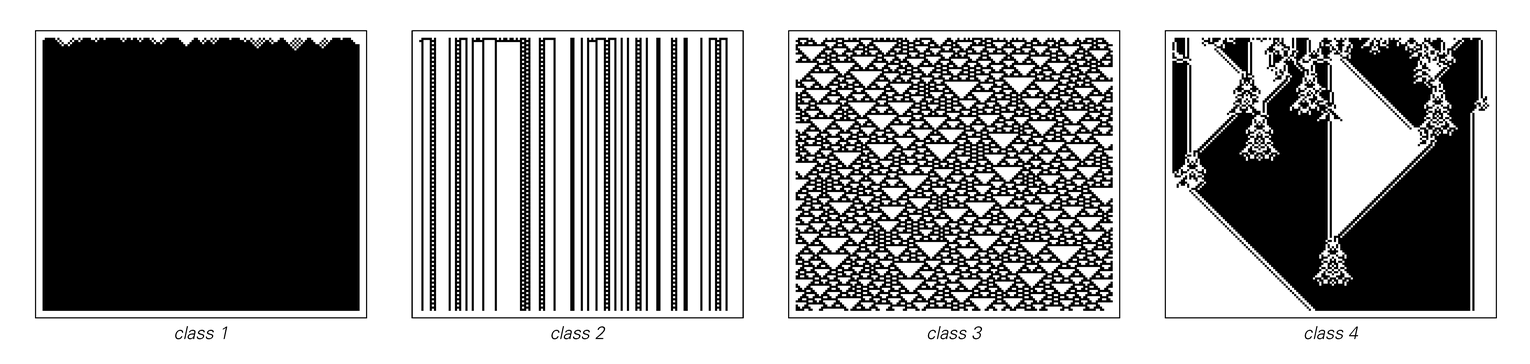
\includegraphics[scale=0.355]{resources/clasificacion_AC.png}
			\caption{Ejemplo de la clasificación de los autómatas celulares}\label{fig:picture}
		\end{figure}
	
	\newpage
		
	\section{Programa}	
		\subsection{Descripción}
		Para este primer programa se ha creado nuestro primer autómata celular, el autómata celular a crear debido a sus características se le conoce como un autómata celular elemental (ECA) que se regirá por la regla 30 (hay 256 reglas de la 0 hasta la 255), pero ¿Cuáles son esas características para que nuestro autómata celular sea considerado como un ECA? Las características son las siguientes:
		\begin{itemize}
    		\item Espacio unidimensional.
		    \item Tiene dos posibles estados o valores para cada célula (0 o 1).
		    \item La reglas que dependen solo de los valores del vecino más cercano.
		    \item Es de tipo frontera periódica o circular.
		\end{itemize}\par
		Nuestro ECA sera regido por la regla 30 o 00011110$_2$, la cual nos estable nuestra función local, es decir, nos define como las células cambiaran de estado en la siguiente iteración dependiendo de los estados o valores de la generación anterior teniendo en cuenta que necesitaremos de una célula central y dos células vecinas, una a cada lado, por lo que el comportamiento seria el siguiente:
		\begin{figure}[H]
			\centering
			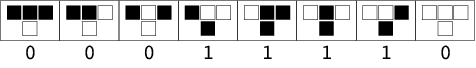
\includegraphics[scale=0.7]{resources/ElementaryCA30Rules_750.png}
			\caption{Comportamiento de la regla 30}\label{fig:picture}
		\end{figure}
		En la imagen 3 podemos ver 8 figuras diferentes entre si, si vemos la primera fila compuesta de 3 células son las combinaciones posibles de los estados (0 o 1, blanco o negro) la célula de abajo nos da el estado que poseerá la hija de la siguiente iteración, es decir, si encontramos 3 células con estado 1 (color negro) en la siguiente iteración nos generaran una célula con el estado 0 (color blanco) o por ejemplo si encontramos que nuestras dos primeras células tienen estado 0 y la ultima tiene el estado 1 entonces la célula de la próxima iteración tendrá el valor 1.\par

		Para el desarrollo de este programa se uso el lenguaje de programación Python usando Tkinter y Matplotlib para la creación de nuestra GUI y las gráficas correspondientes, el entorno de desarrollo utilizado fue Visual Studio Code. Mencionar que aunque nuestro programa nos permite usar cualquiera de las 256 reglas, en esta ocasión solo nos enfocaremos en la regla 30. Mencionar que nuestro archivo principal y el que se debe de ejecutar es el archivo con el nombre Interfaz.py ya que el archivo Logica.py solo contiene la parte lógica del programa y parte de la graficacón de los resultados.
		\newpage
		\subsection{Pruebas}
		Este programa tiene varios aspectos que han sido cubiertos. Para iniciar las pruebas
crearemos un autómata de 1000 células con 1000 iteraciones, algo especial de este autómata es que tenemos solo una célula con valor 1 en medio de todas las demás células que tienen valor 0.
		\begin{figure}[H]
			\centering
			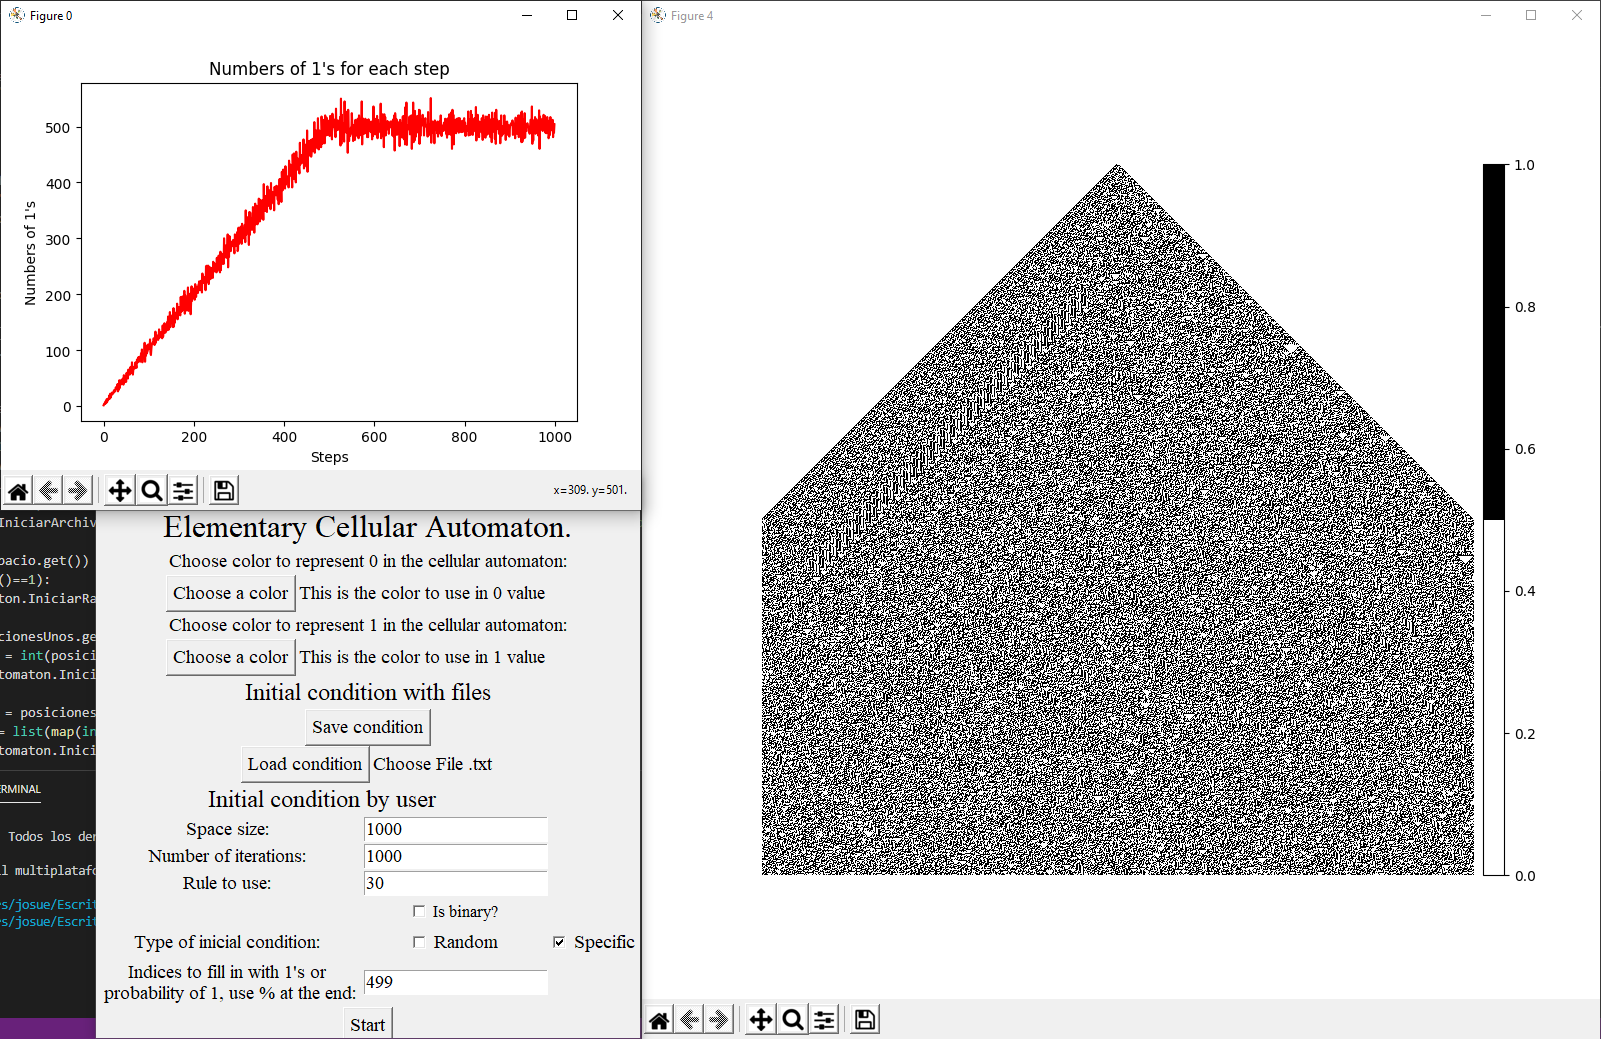
\includegraphics[scale=0.42]{resources/prueba1.png}
			\caption{ECA con solo una célula con valor 1. Regla 30}\label{fig:picture}
		\end{figure}
		Como vemos en la figura 4 tenemos en el lado derecho de la imagen nuestro ECA resultante después de aplicar 1000 iteraciones con la regla 30 y en la parte superior izquierda tenemos el crecimiento de células con valor 1 durante esas 1000 iteraciones, podemos apreciar que su crecimiento nos recuerda a un crecimiento logarítmico. En ambas gráficas tenemos la posibilidad de agrandar el tamaño mediante el icono de la lupa que tenemos en la parte inferior de ambas ventanas, una vez seleccionada la lupa podremos seleccionar un área rectangular en nuestra gráfica para poder agrandar lo que abarque dicha área, esto con el fin de visualizar aun mejor nuestro autómata y el crecimiento de nuestras células con valor 1 como se ve en la figura 5.
		\begin{figure}[H]
			\centering
			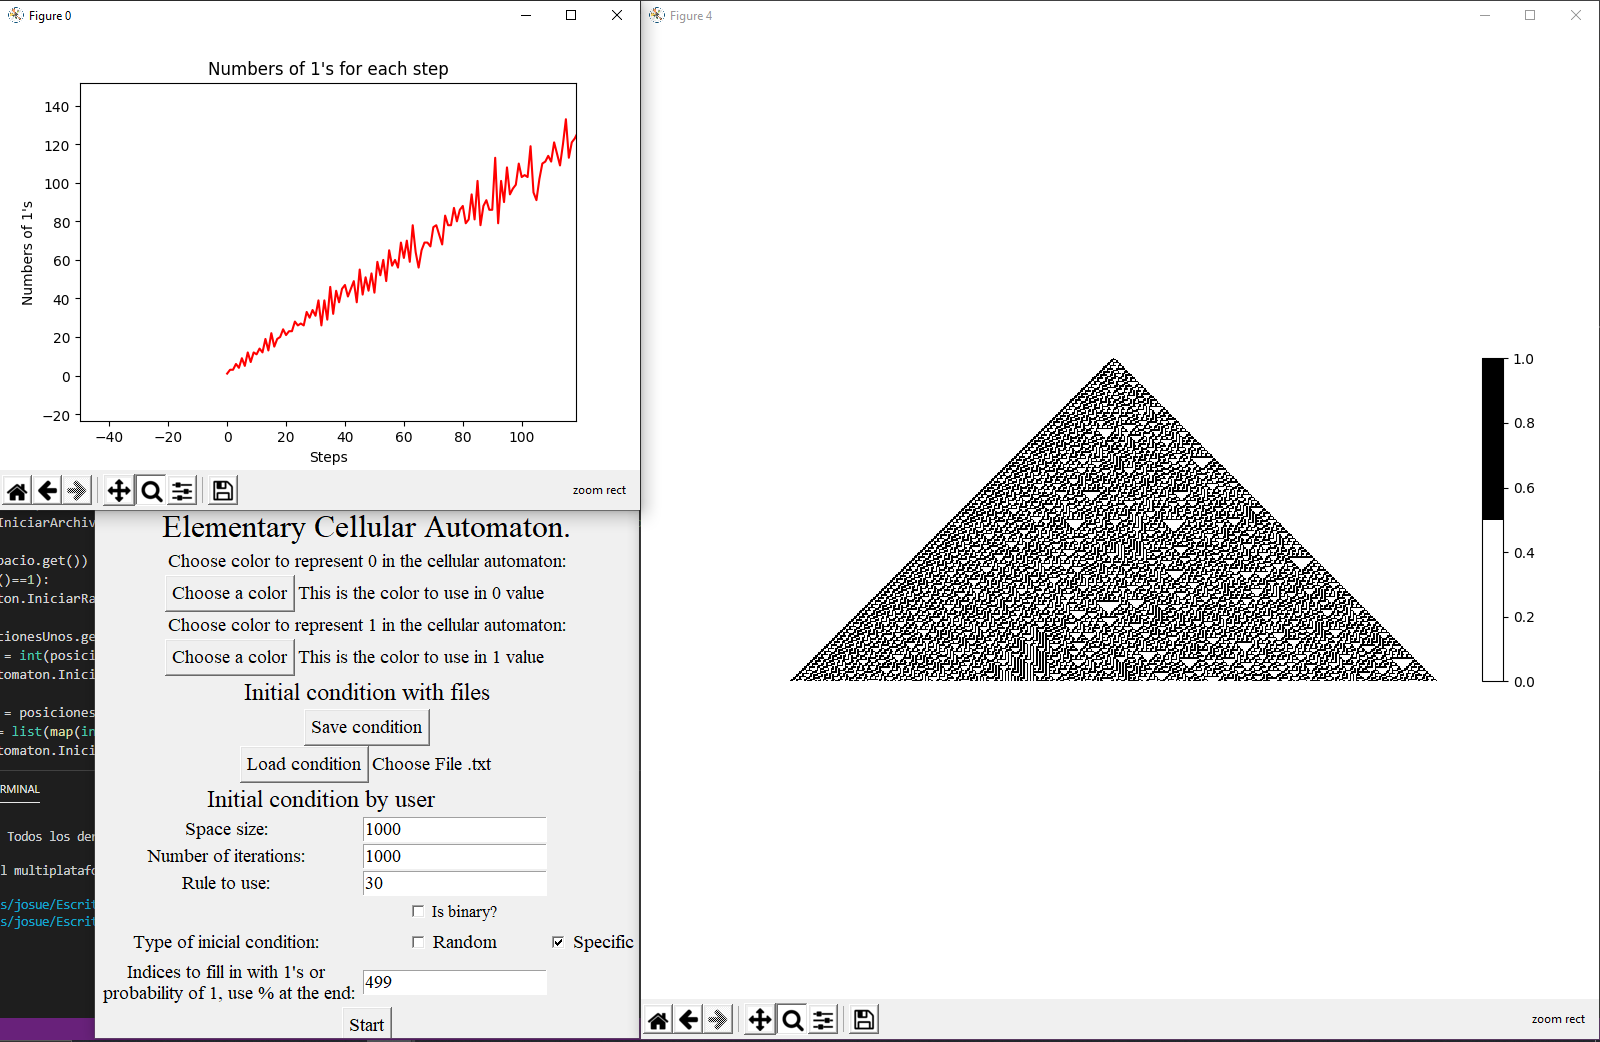
\includegraphics[scale=0.42]{resources/prueba2.png}
			\caption{ECA con solo una célula con valor 1 agrandando el tamaño para poder visualizar aun mejor el comportamiento. Regla 30}\label{fig:picture}
		\end{figure}
		Nuestro programa también nos permite guardar nuestra configuración de nuestro ECA, en este caso solo toma la iteración 0 y es guardado en un archivo con el siguiente nombre $"$celulasIniciales.txt$"$ en caso de existir sobre escribirá la nueva información, en caso contrario lo creara desde cero, mencionar que si se desea se puede modificar el nombre pero no la extensión posterior de haber creado el archivo. En este caso nuestro programa nos arroja un mensaje diciendo que el archivo fue guardo exitosamente y se nos crea un archivo con el nombre y extensión anteriormente mencionados (ver figura 6 y 7).
		\begin{figure}[H]
			\centering
			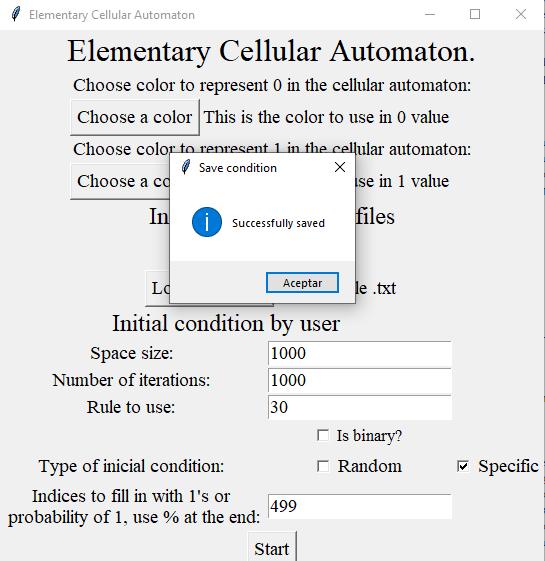
\includegraphics[scale=0.42]{resources/archivoSave.png}
			\caption{Iteración 0 de nuestro ECA guardada exitosamente}\label{fig:picture}
		\end{figure}
		\begin{figure}[H]
			\centering
			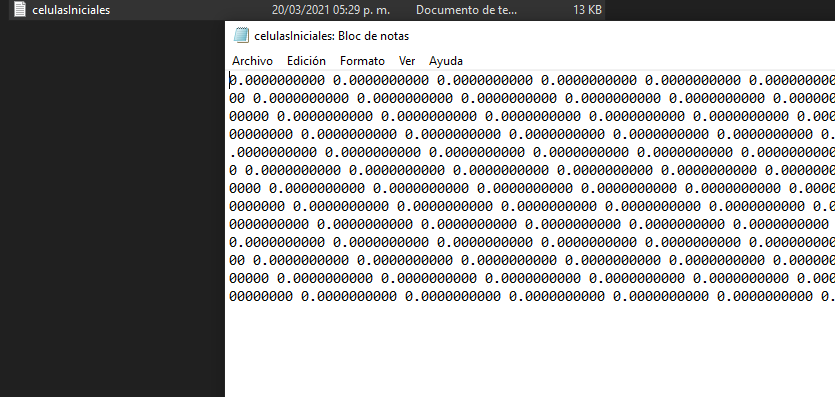
\includegraphics[scale=0.5]{resources/archivoSave2.png}
			\caption{Contenido del archivo}\label{fig:picture}
		\end{figure}
		También como era de esperarse se puede cargar archivo de texto al programa para volver a usarlo, algo importante a mencionar es que no guarda ni el numero de iteraciones, los colores para los valores 0 y 1 ni la regla usada esto con fines de facilitar al usuario poder usar un mismo inicio con diferentes reglas y numero de iteraciones cada vez que le plazca hacerlo. En la figura 8 cargamos nuestro archivo y solo modificamos el color que se le asigna a los valores 0 y 1, colocamos la regla a usar (regla 30) y nuestro numero de iteraciones sera de nuevo 1000, el panel para poder elegir el color se puede observar en la figura 9.
		\begin{figure}[H]
			\centering
			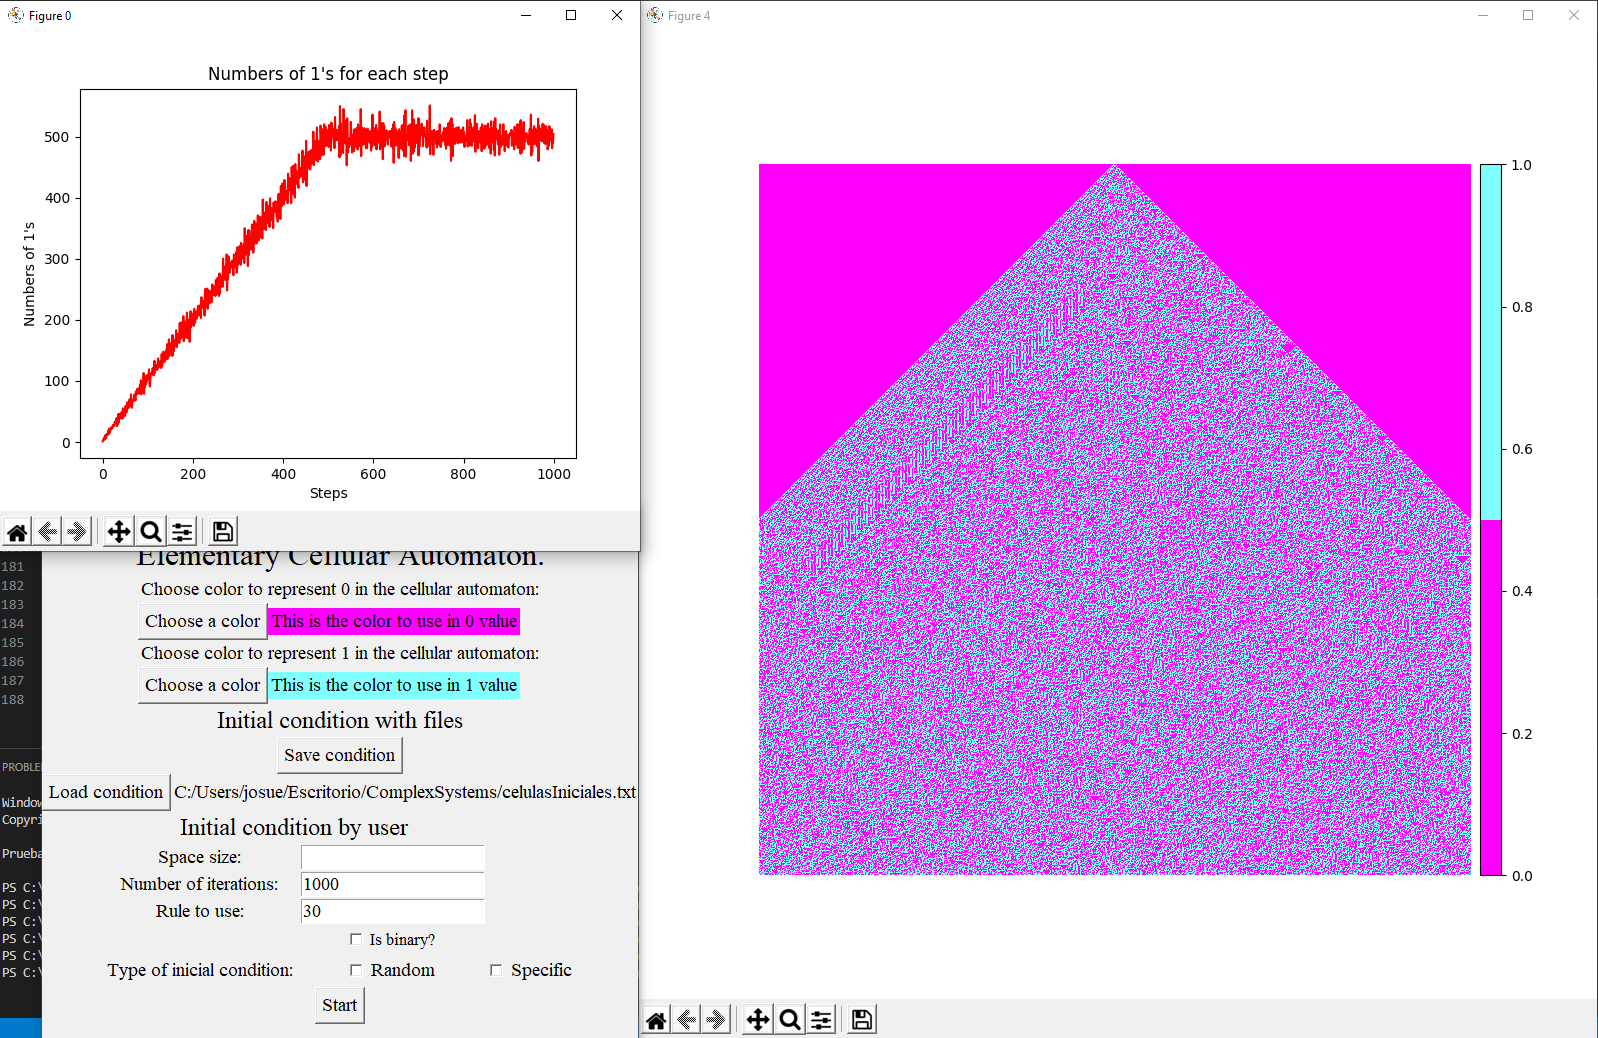
\includegraphics[scale=0.42]{resources/automataHappy.png}
			\caption{ECA con diferentes colores para los valores 0 y 1}\label{fig:picture}
		\end{figure}
		\begin{figure}[H]
			\centering
			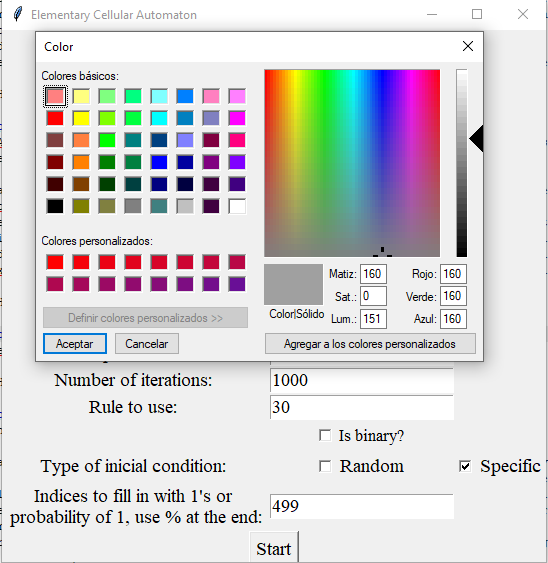
\includegraphics[scale=0.5]{resources/elegirColor.png}
			\caption{Panel para poder elegir color para valores 0 y 1}\label{fig:picture}
		\end{figure}
		Realizando otra prueba crearemos un ECA con un tamaño de 500 células con 500 iteraciones, pero en esta ocasión la regla 30 sera ingresada como numero binario (00011110$_2$) y serán asignadas células con valor 1 de forma aleatoria.
		\begin{figure}[H]
			\centering
			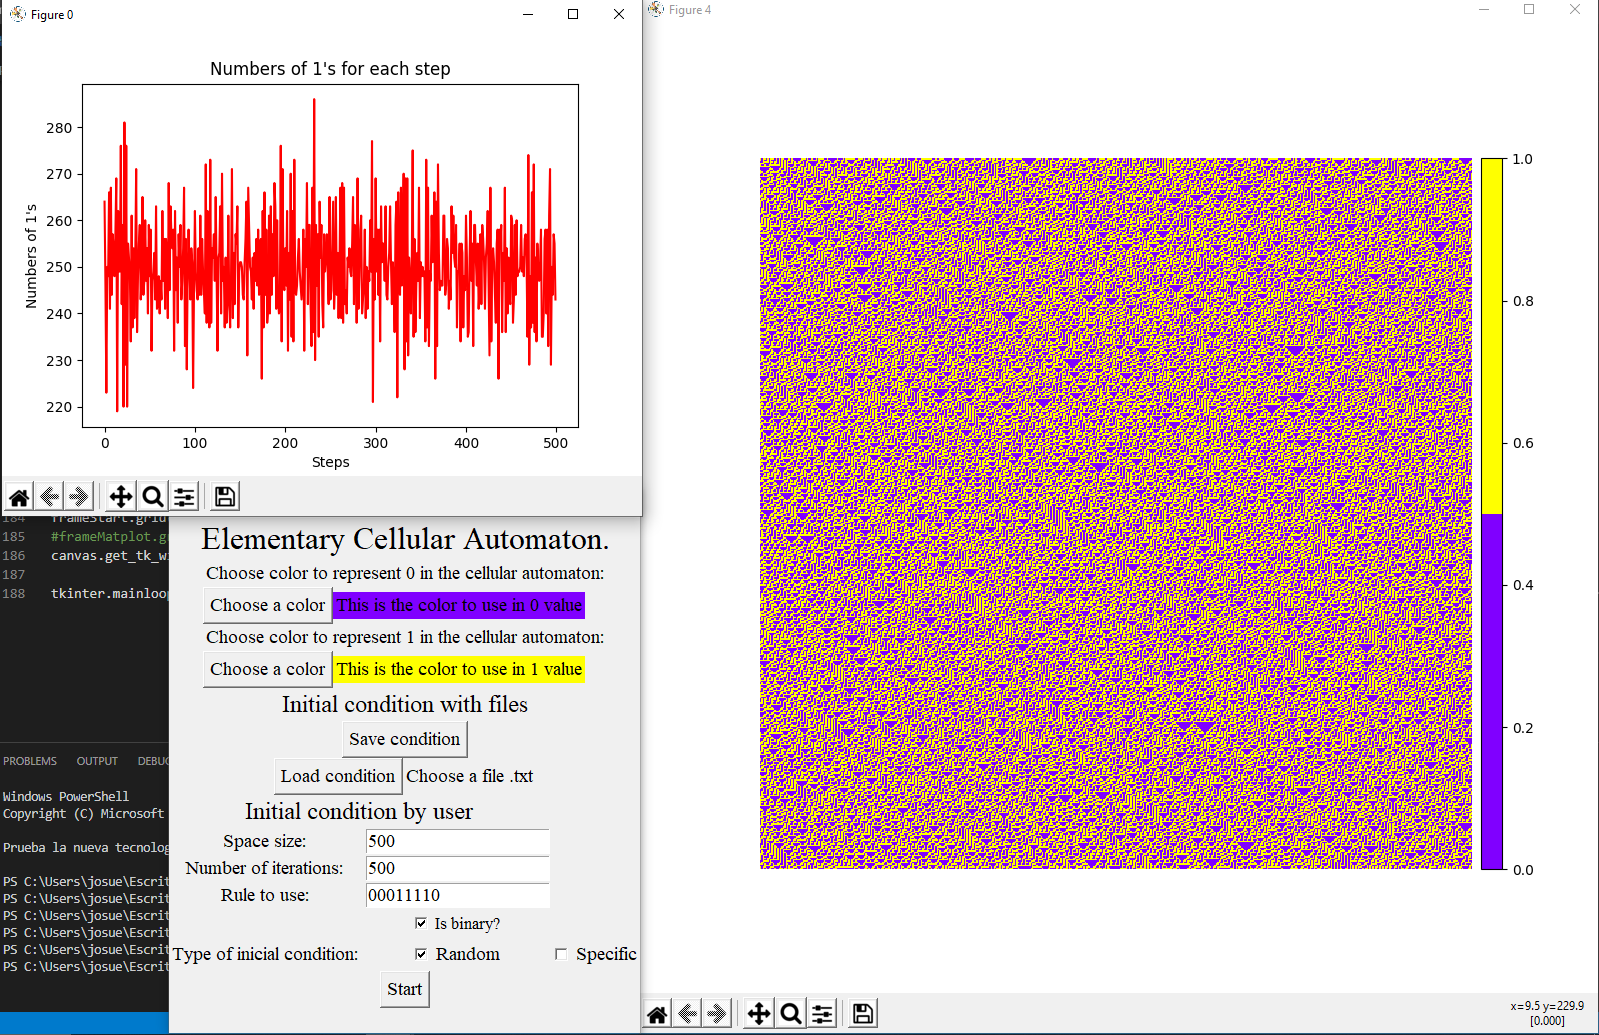
\includegraphics[scale=0.42]{resources/pruebaF.png}
			\caption{ECA de 500 células por 500 iteraciones creado de forma aleatoria}								\label{fig:picture}
		\end{figure}
		Como ultimas pruebas realizaremos lo siguiente:  mediante las reglas 15, 22, 30, 54, 110 y 126 para la construcción de nuestro ECA mostraremos 3 evoluciones por cada regla en espacios de 400 células por 400 iteraciones, una empezara con un uno al centro, otra iniciando con un 50\% de probabilidad de unos y la última iniciando con un 95\% de probabilidad de unos.\par
		Empecemos así con nuestra regla 15, veremos a través de de las imágenes 11 a la 14 el comportamiento de nuestro ECA con base en donde se encuentren las células iniciales con valor 1.
		\begin{figure}[H]
			\centering
			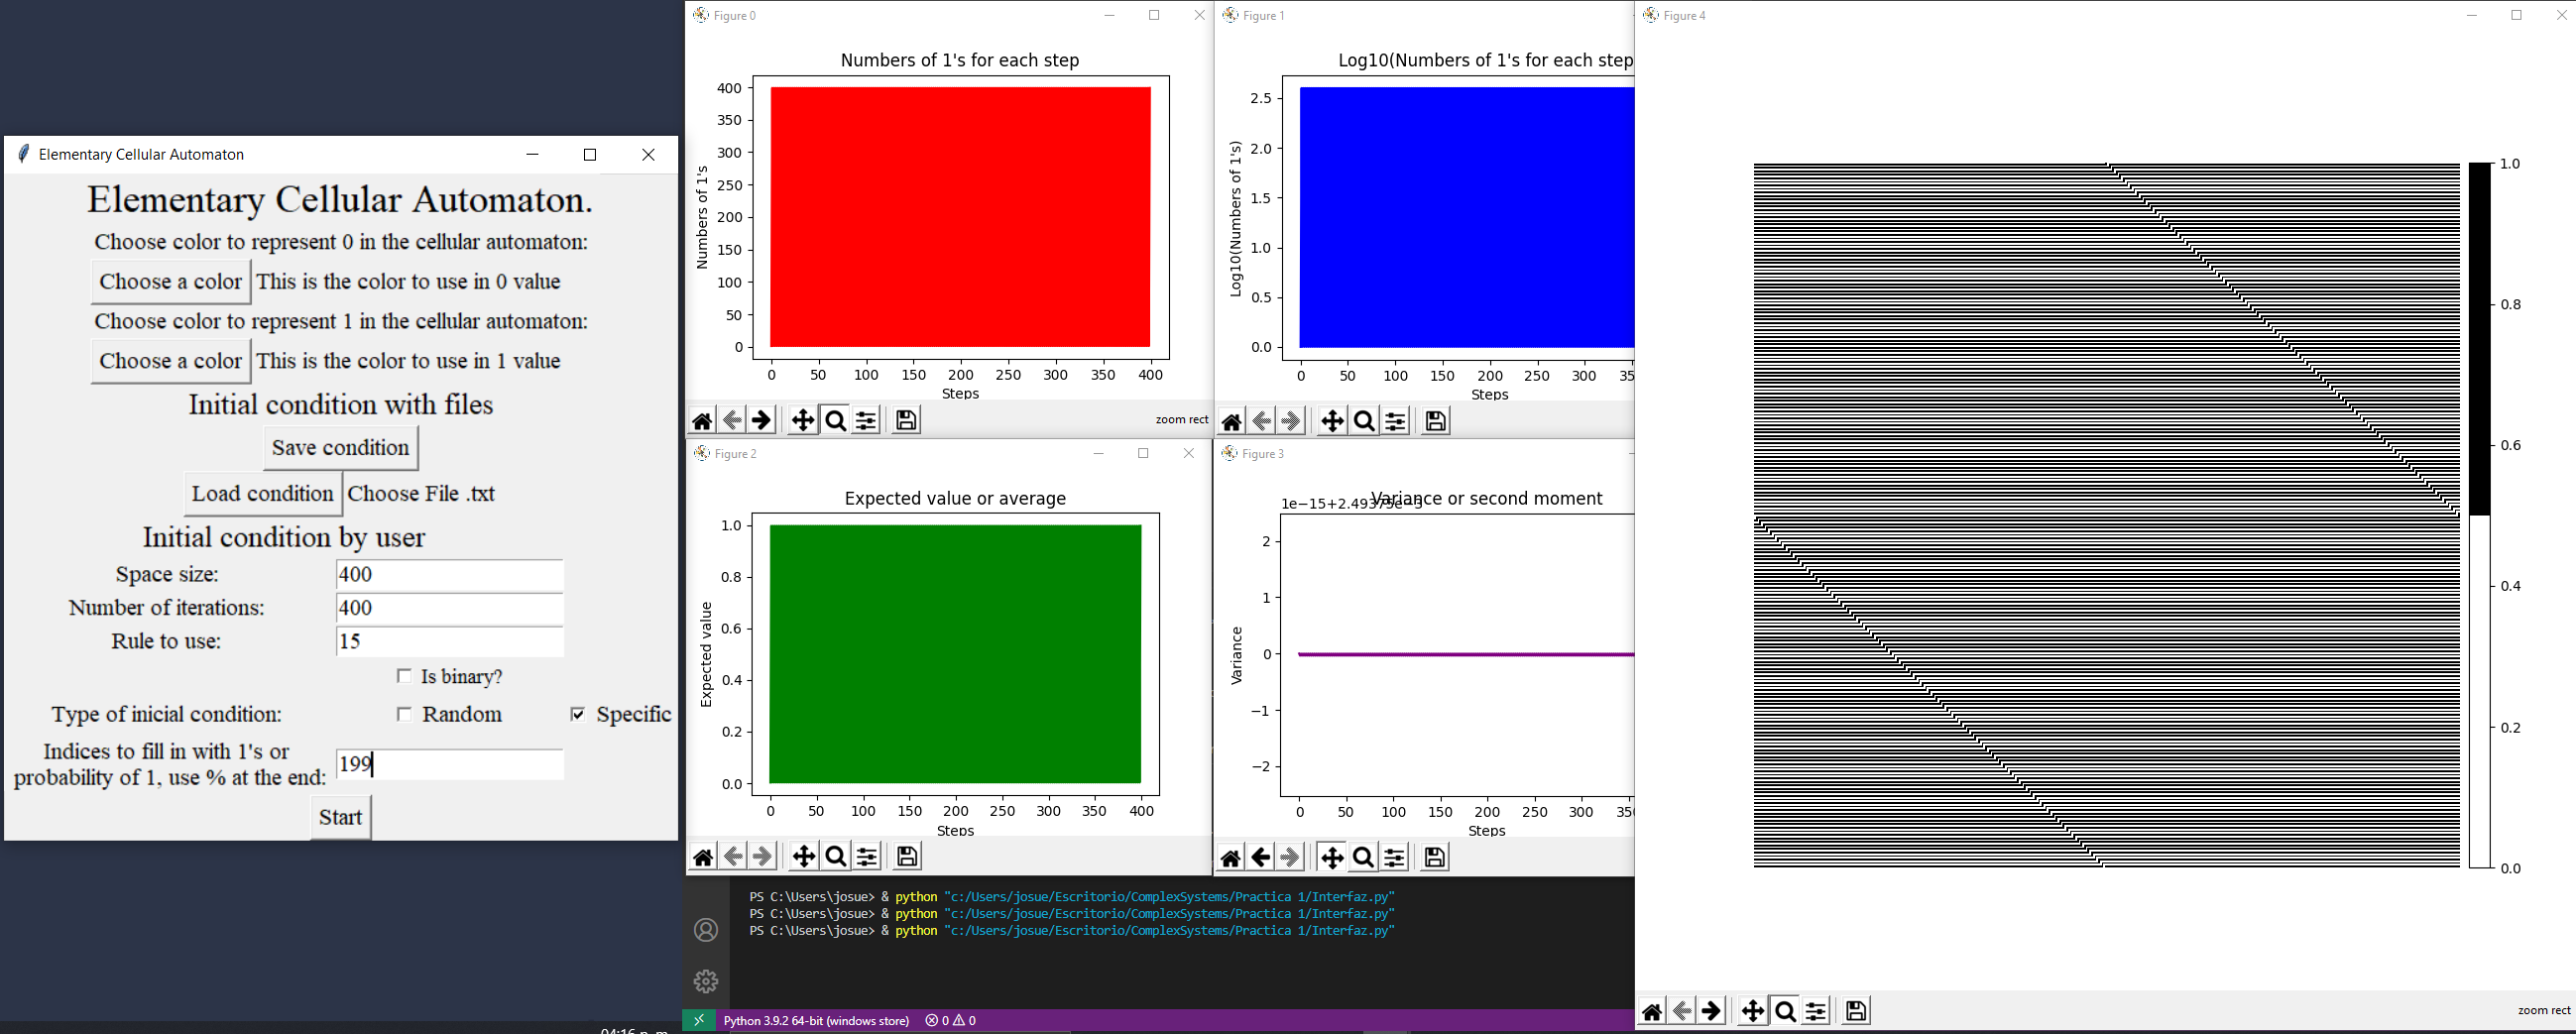
\includegraphics[scale=0.26]{resources/add1.png}
			\caption{ECA de 400 células por 400 iteraciones con una célula inicial central, regla 15}								\label{fig:picture}
		\end{figure}
		Para visualizar mejor la información nuestras gráficas hagamos una ampliación de las mismas para las primeras 50 iteraciones.
		\begin{figure}[H]
			\centering
			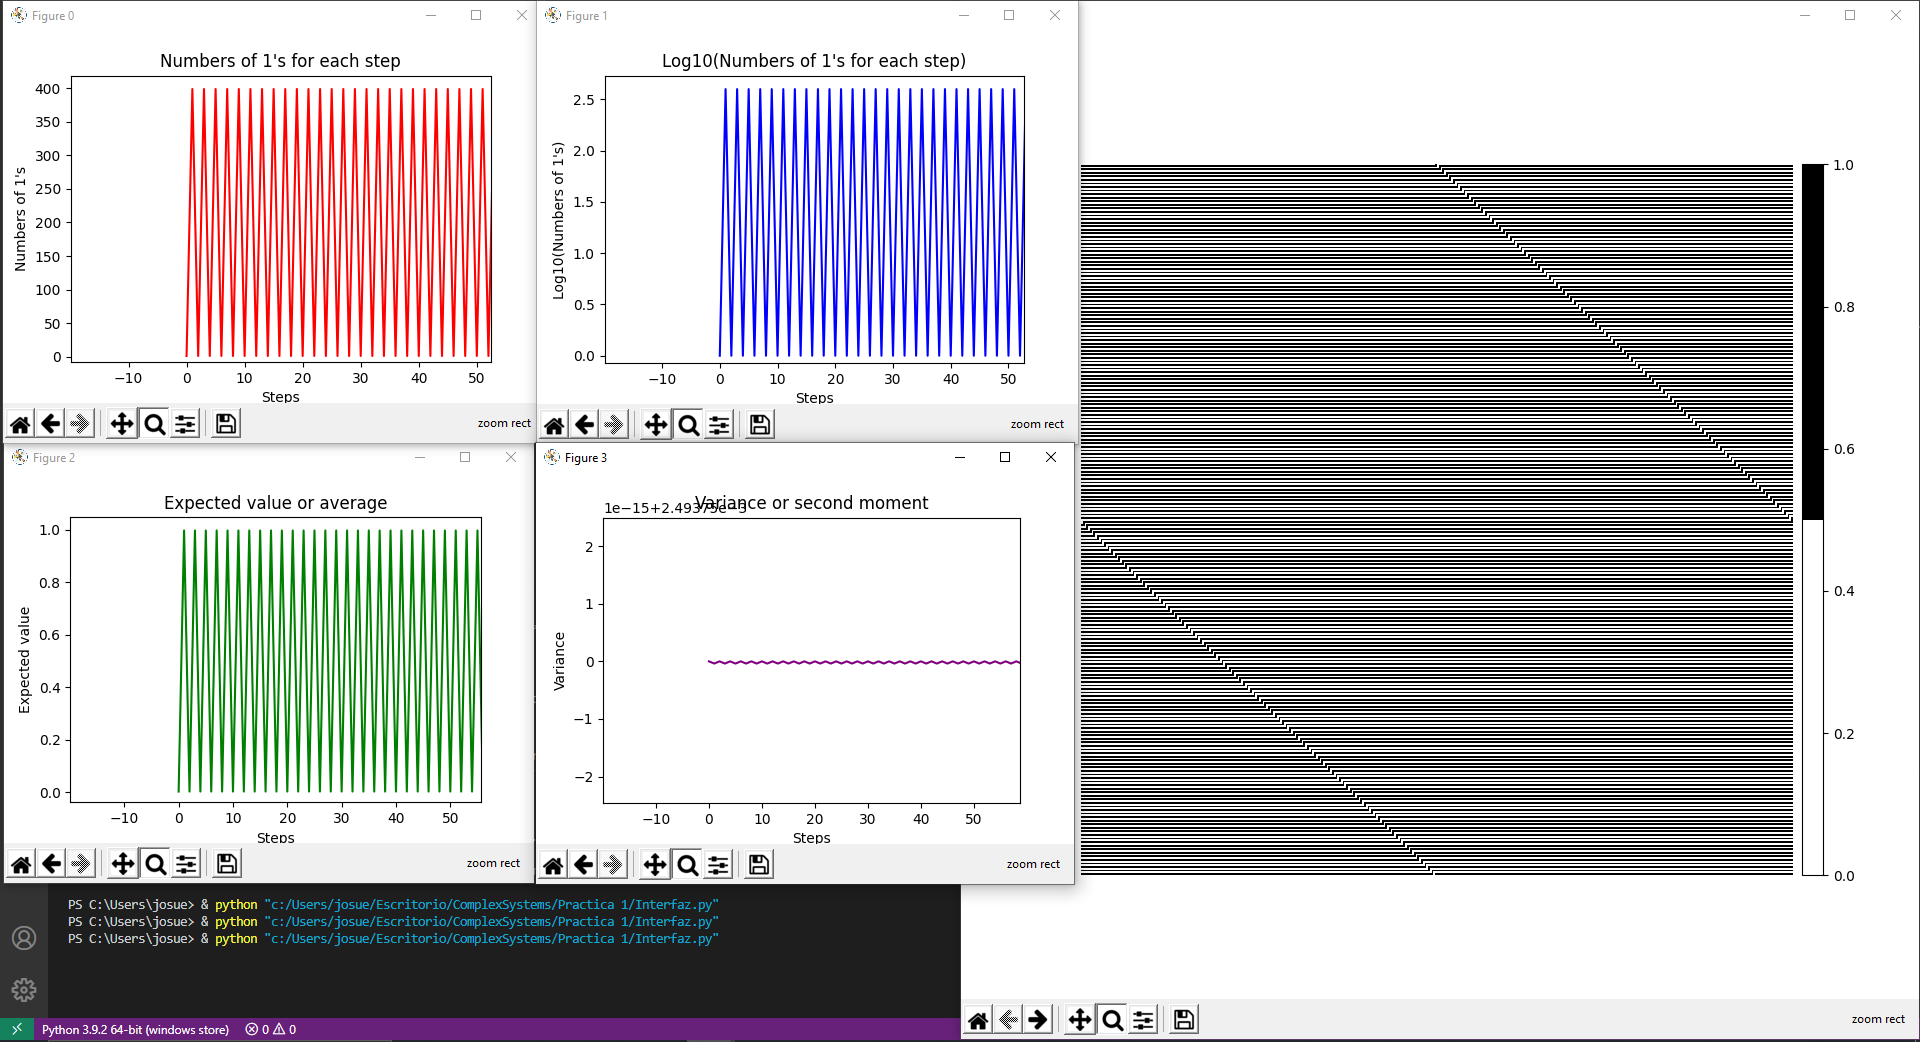
\includegraphics[scale=0.35]{resources/add1z.png}
			\caption{ECA de 400 células por 400 iteraciones con una célula inicial central con aumento, regla 15}								\label{fig:picture}
		\end{figure}
		Como vemos el comportamiento de nuestro ECA es de una forma constante y es que en la iteración tenemos 1 célula viva a pasar a tener 399 células y a la siguiente volvemos a tener solo una, como si de un ciclo se tratase.\par
		Pasando a la siguiente prueba, usaremos el 50\% de unos y observemos su comportamiento
		\begin{figure}[H]
			\centering
			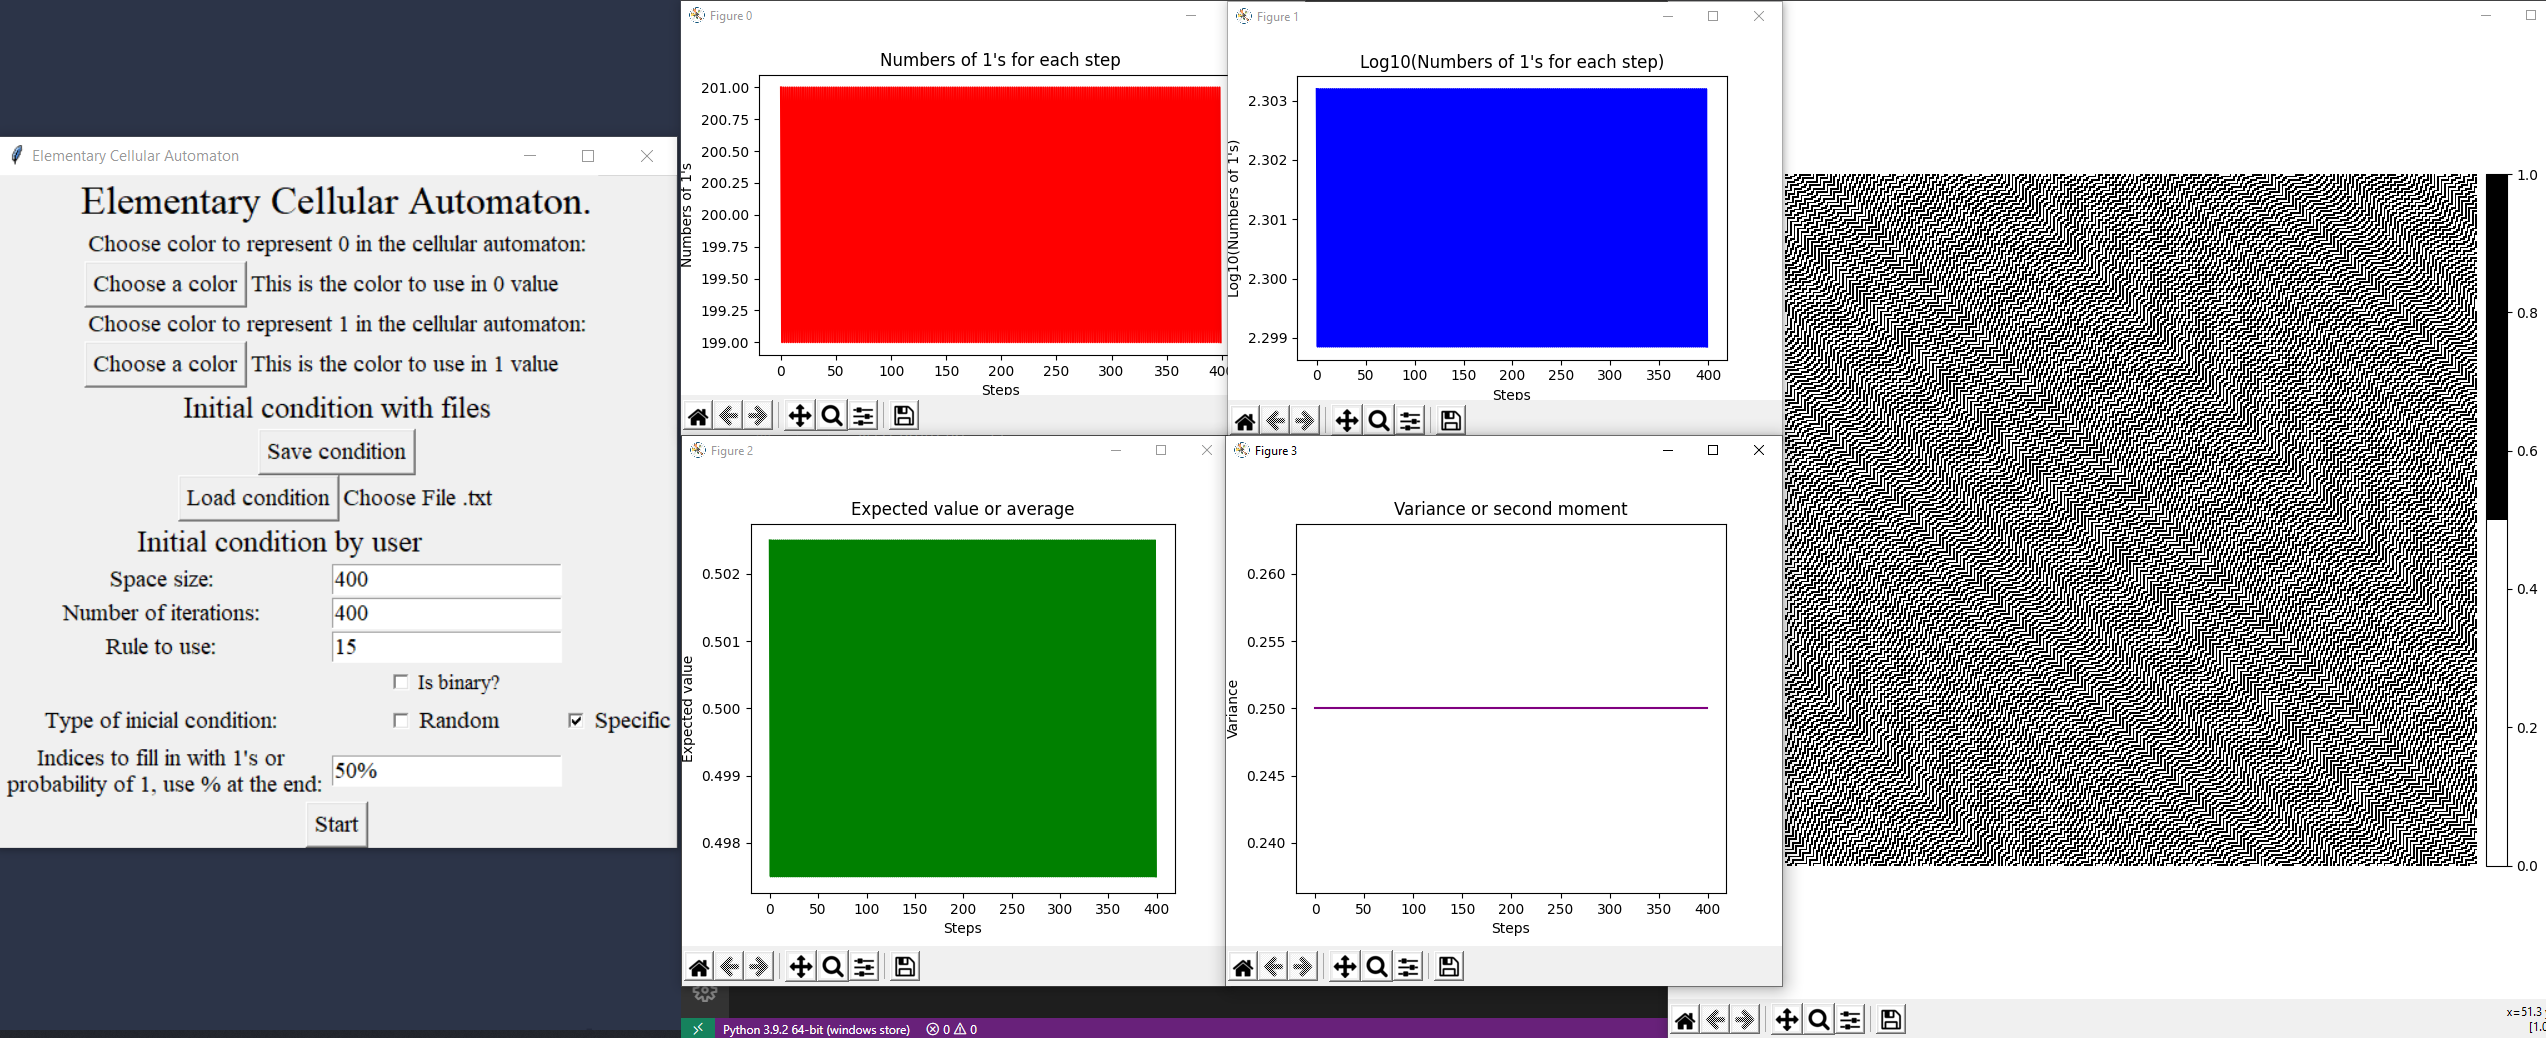
\includegraphics[scale=0.26]{resources/add2.png}
			\caption{ECA de 400 células por 400 iteraciones con 50\% de probabilidad de 1's, regla 15}								\label{fig:picture}
		\end{figure}		
		Como vemos tiene un comportamiento similar a la primera prueba solo que el numero de células vivas por iteración cambiaron, ahora son menos que en la prueba anterior.
		Como ultima prueba para esta regla, la probabilidad a usar sera del 95\% así que veamos el resultado
		\begin{figure}[H]
			\centering
			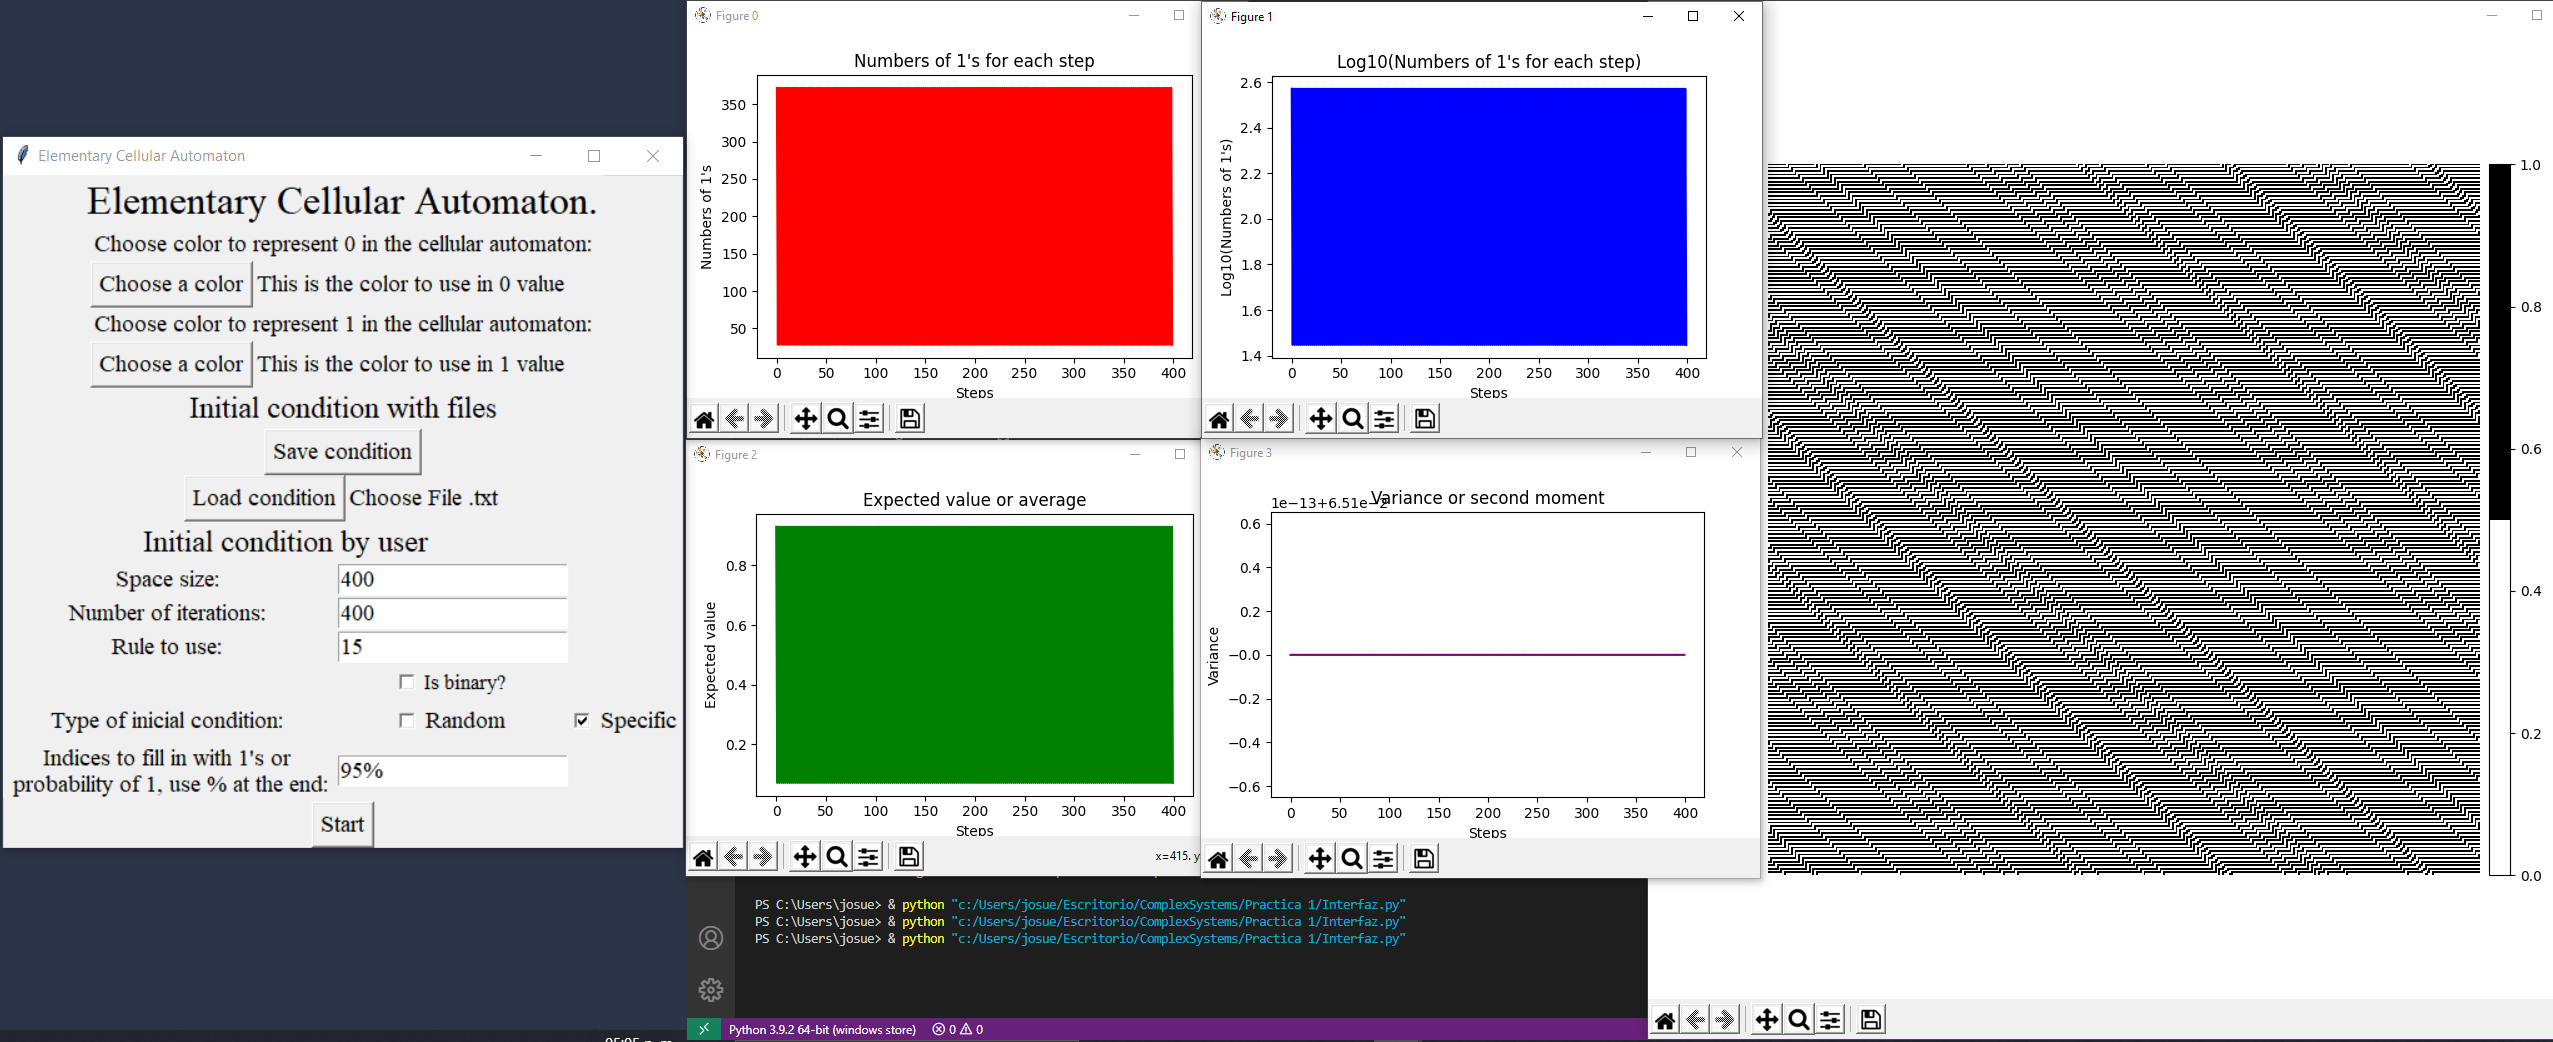
\includegraphics[scale=0.26]{resources/add3.png}
			\caption{ECA de 400 células por 400 iteraciones con 95\% de probabilidad de 1's, regla 15}								\label{fig:picture}
		\end{figure}		
		El resultado nuevamente es muy similar a los anteriores, por lo que podemos suponer que si probamos diferentes configuraciones iniciales siempre serán parecidas, solo cambiaran el numero de 1's.\par
		Continuando con las pruebas, ahora vayamos con la regla 22 de aquí en adelante se mostraran las 3 imágenes correspondientes con los 3 valores iniciales diferentes para posteriormente dar un pequeño estudio de los resultados.
		\begin{figure}[H]
			\centering
			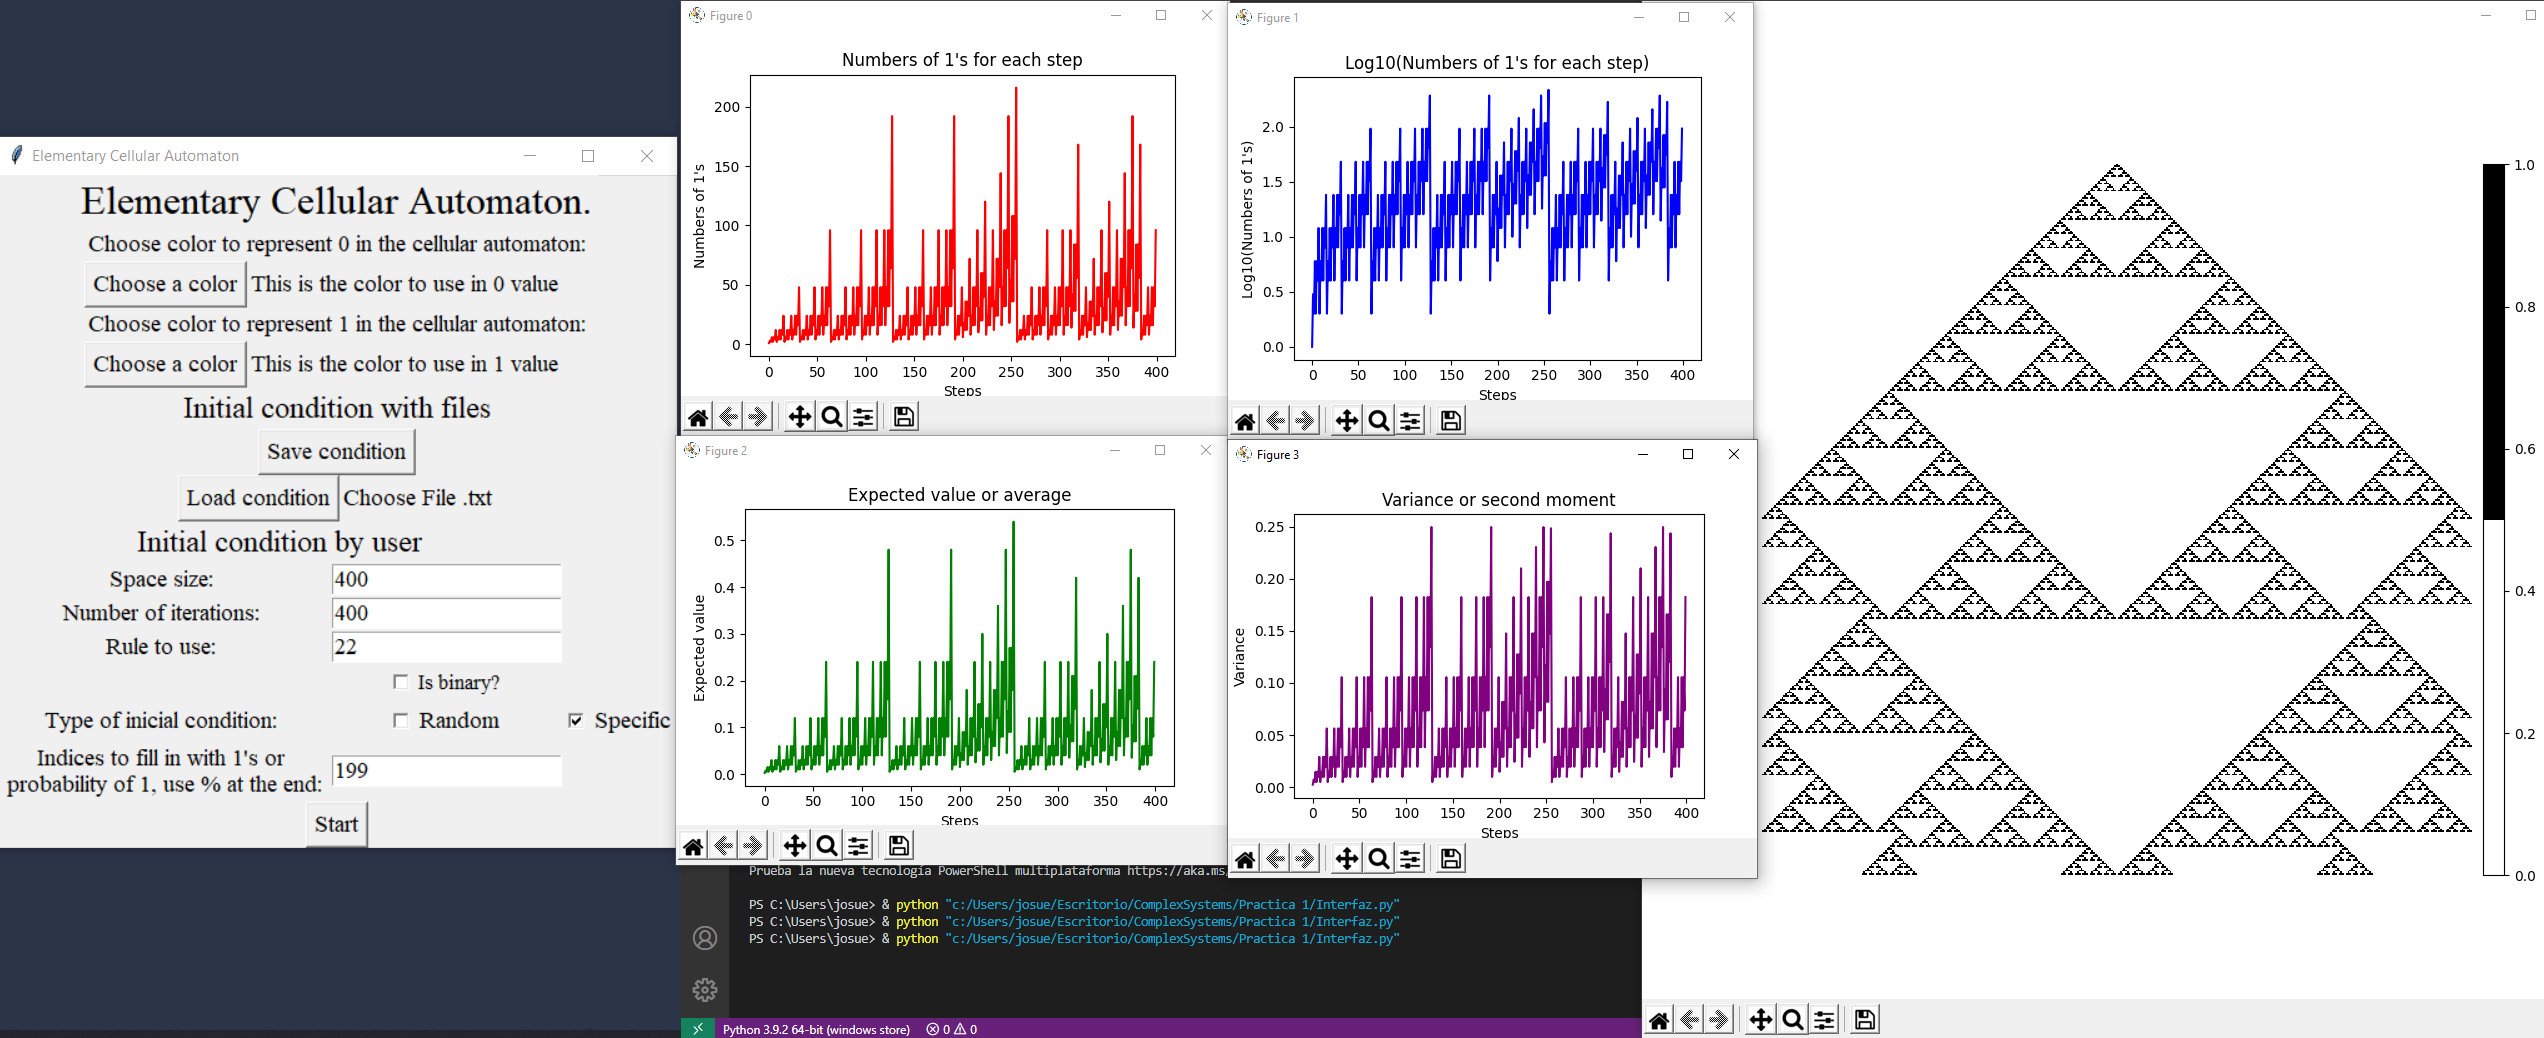
\includegraphics[scale=0.26]{resources/add4.png}
			\caption{ECA de 400 células por 400 iteraciones con una célula inicial central, regla 22}								\label{fig:picture}
		\end{figure}
		\begin{figure}[H]
			\centering
			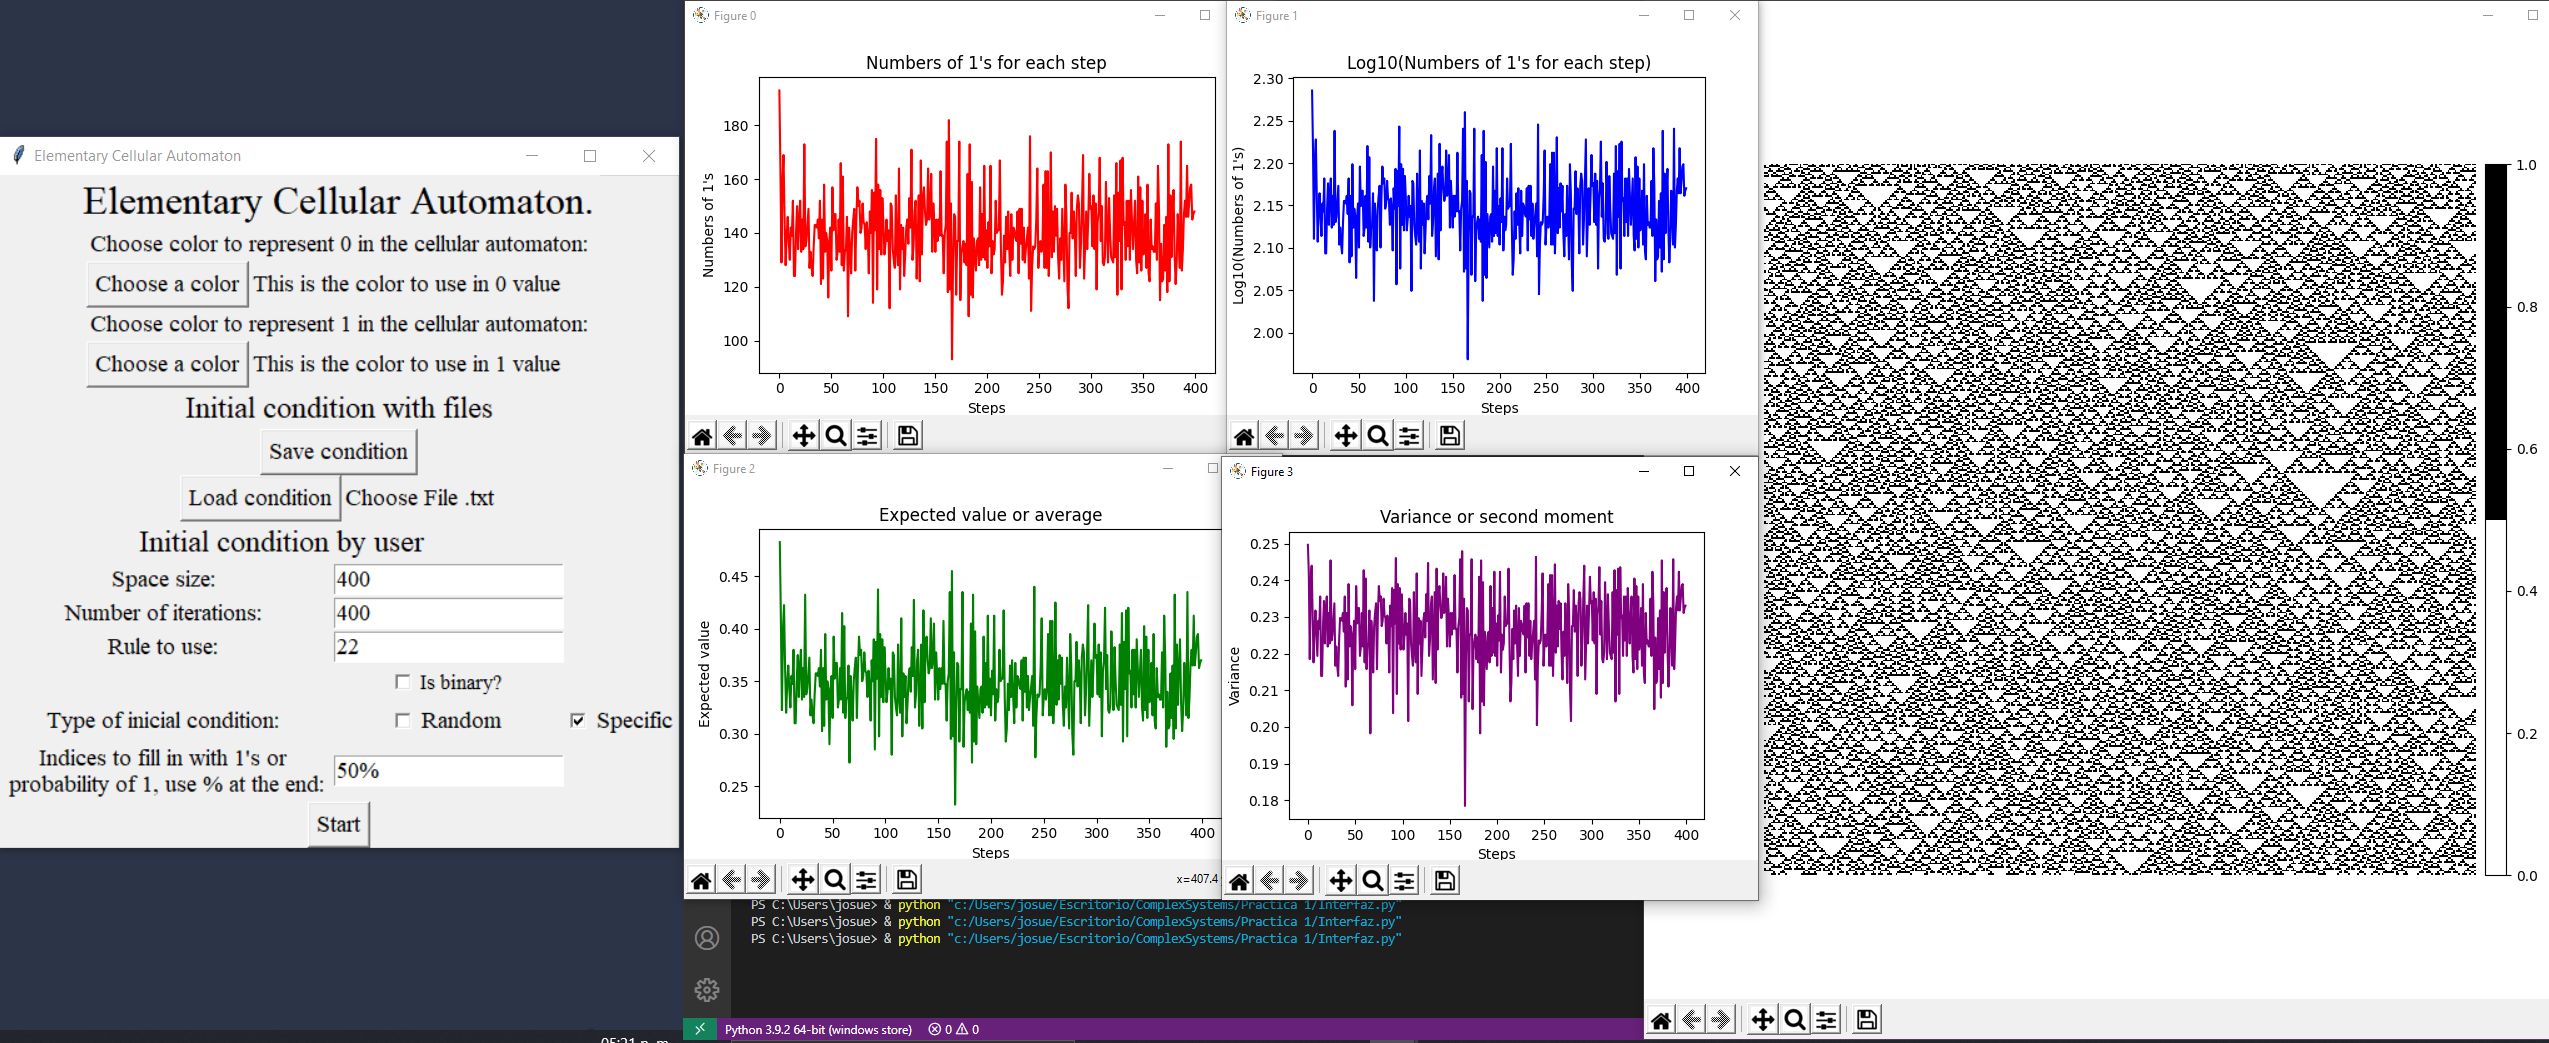
\includegraphics[scale=0.26]{resources/add5.png}
			\caption{ECA de 400 células por 400 iteraciones con 50\% de probabilidad de 1's, regla 22}								\label{fig:picture}
		\end{figure}
		\begin{figure}[H]
			\centering
			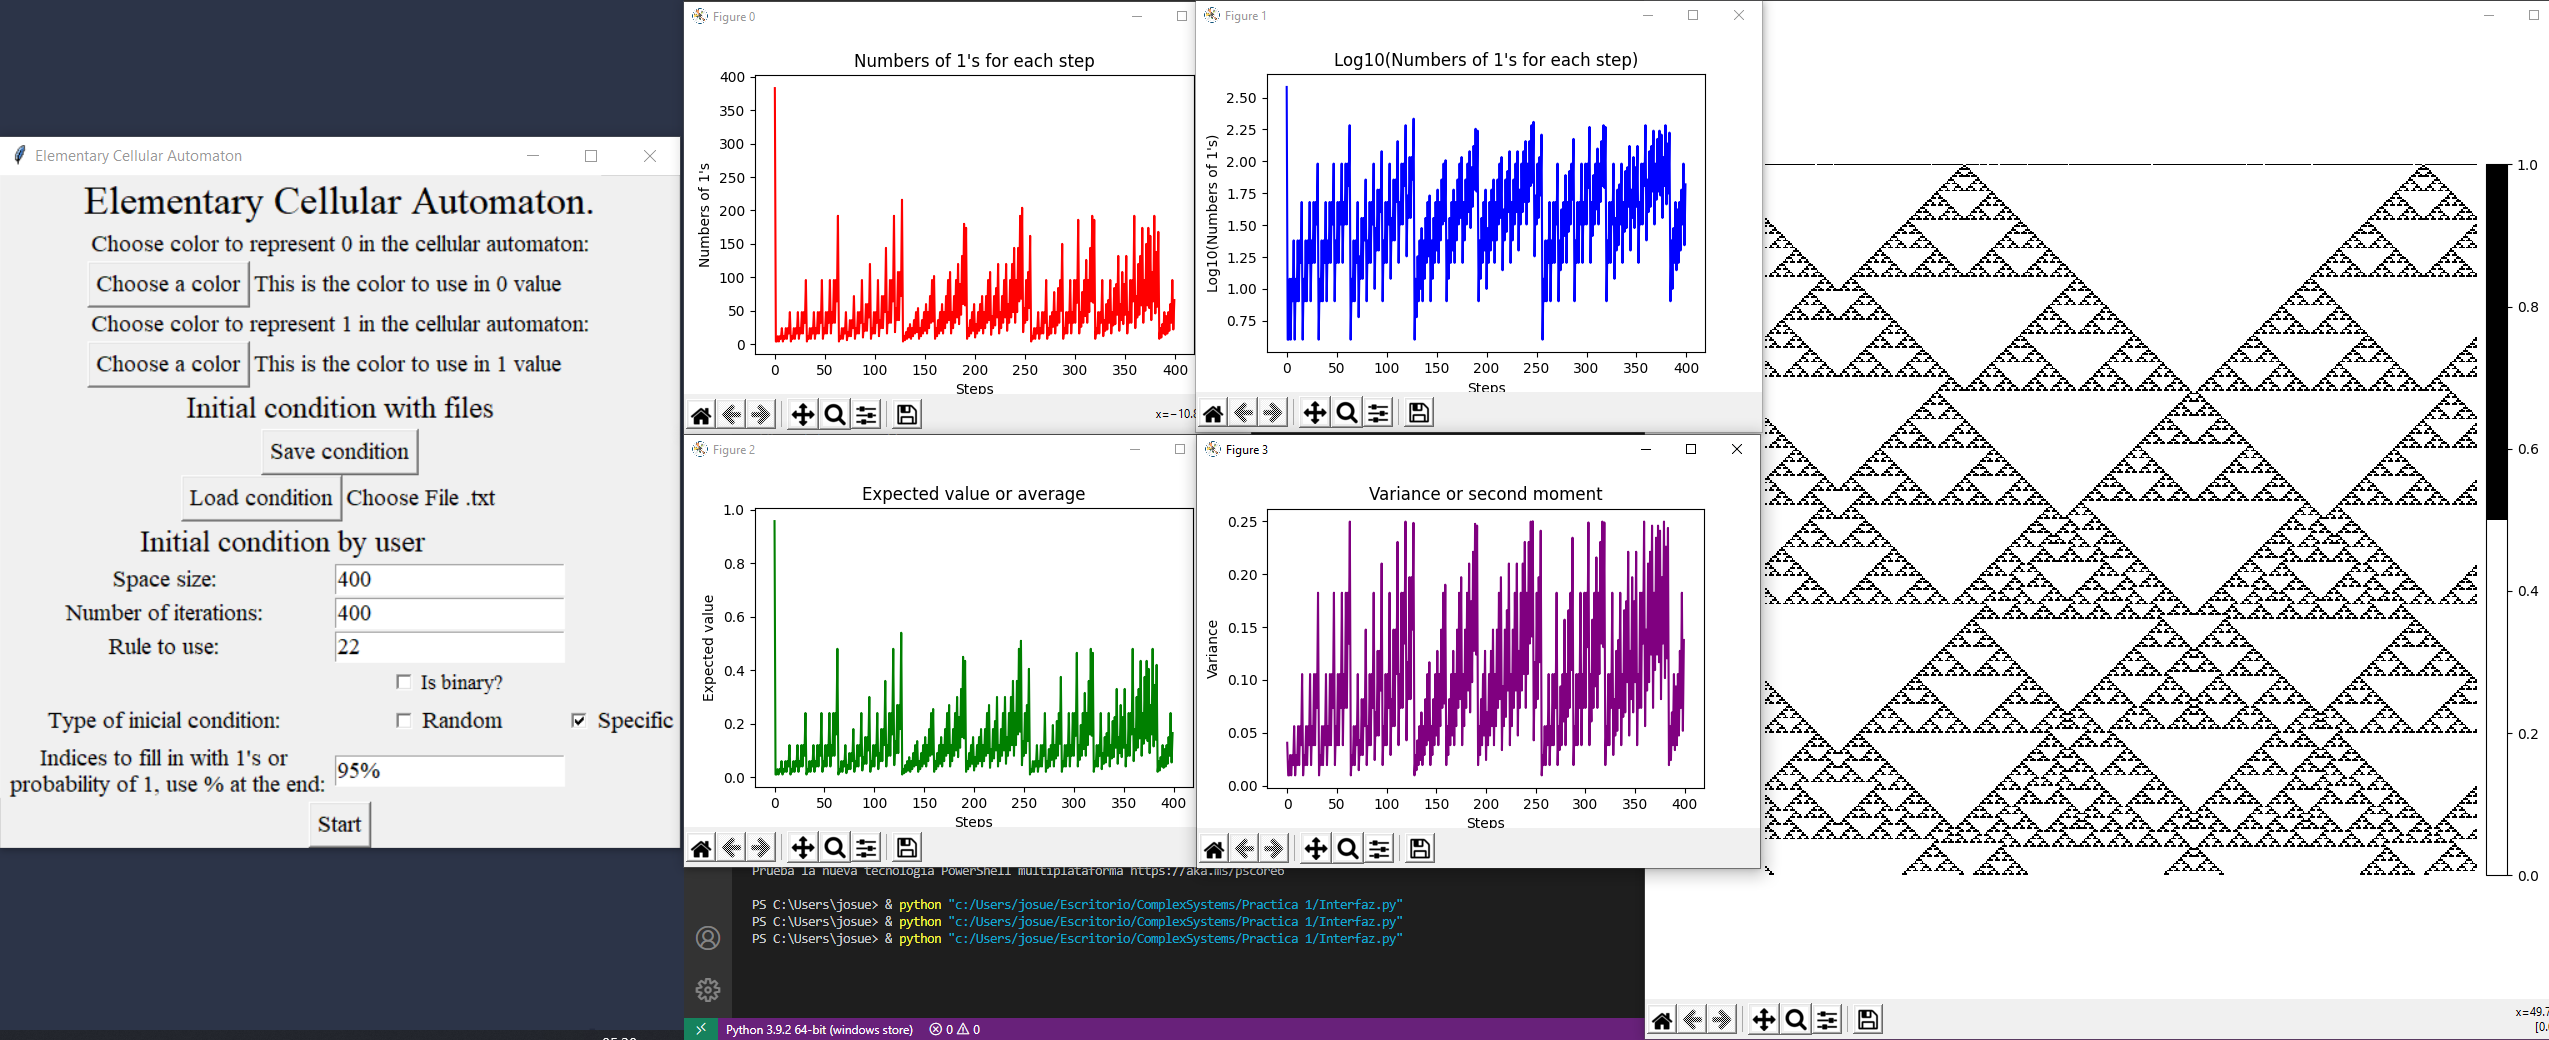
\includegraphics[scale=0.26]{resources/add6.png}
			\caption{ECA de 400 células por 400 iteraciones con 95\% de probabilidad de 1's, regla 22}								\label{fig:picture}
		\end{figure}
		Como se ven desde la figura 15 a la 17 con esta regla si cambia el comportamiento de nuestras gráficas con base a cada tipo de condición inicial, aunque la figura 15 y 17 tiene ciertas similitudes pero no son lo mismo, empezamos a ver que tan influyente es la regla en el comportamiento de nuestro ECA. \par 
		Ahora pasemos a la regla 30 con las mismas pruebas.
		\begin{figure}[H]
			\centering
			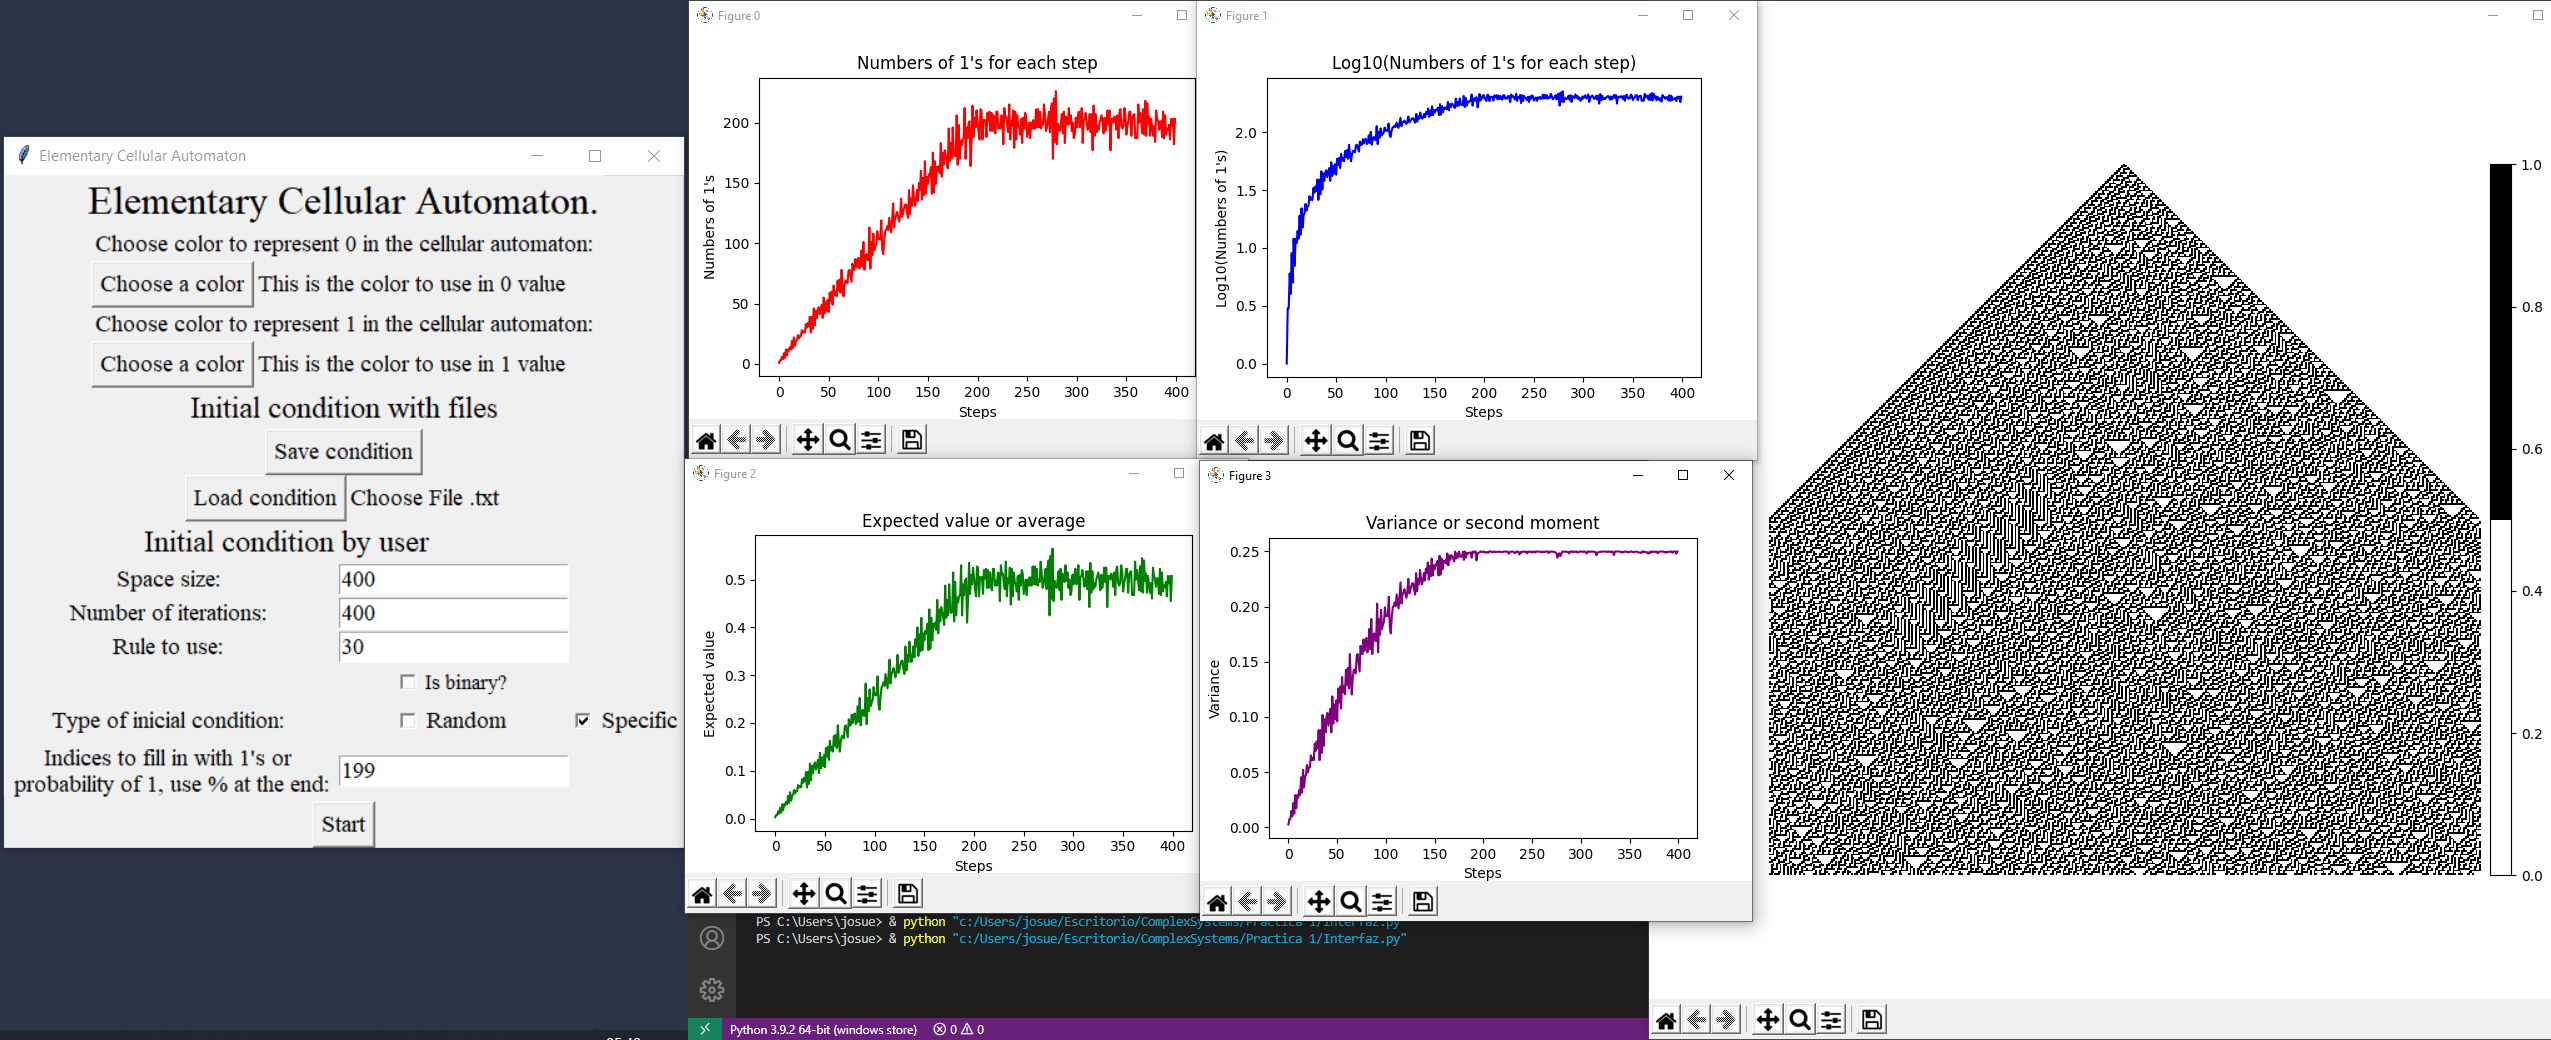
\includegraphics[scale=0.26]{resources/add7.png}
			\caption{ECA de 400 células por 400 iteraciones con una célula inicial central, regla 30}								\label{fig:picture}
		\end{figure}
		\begin{figure}[H]
			\centering
			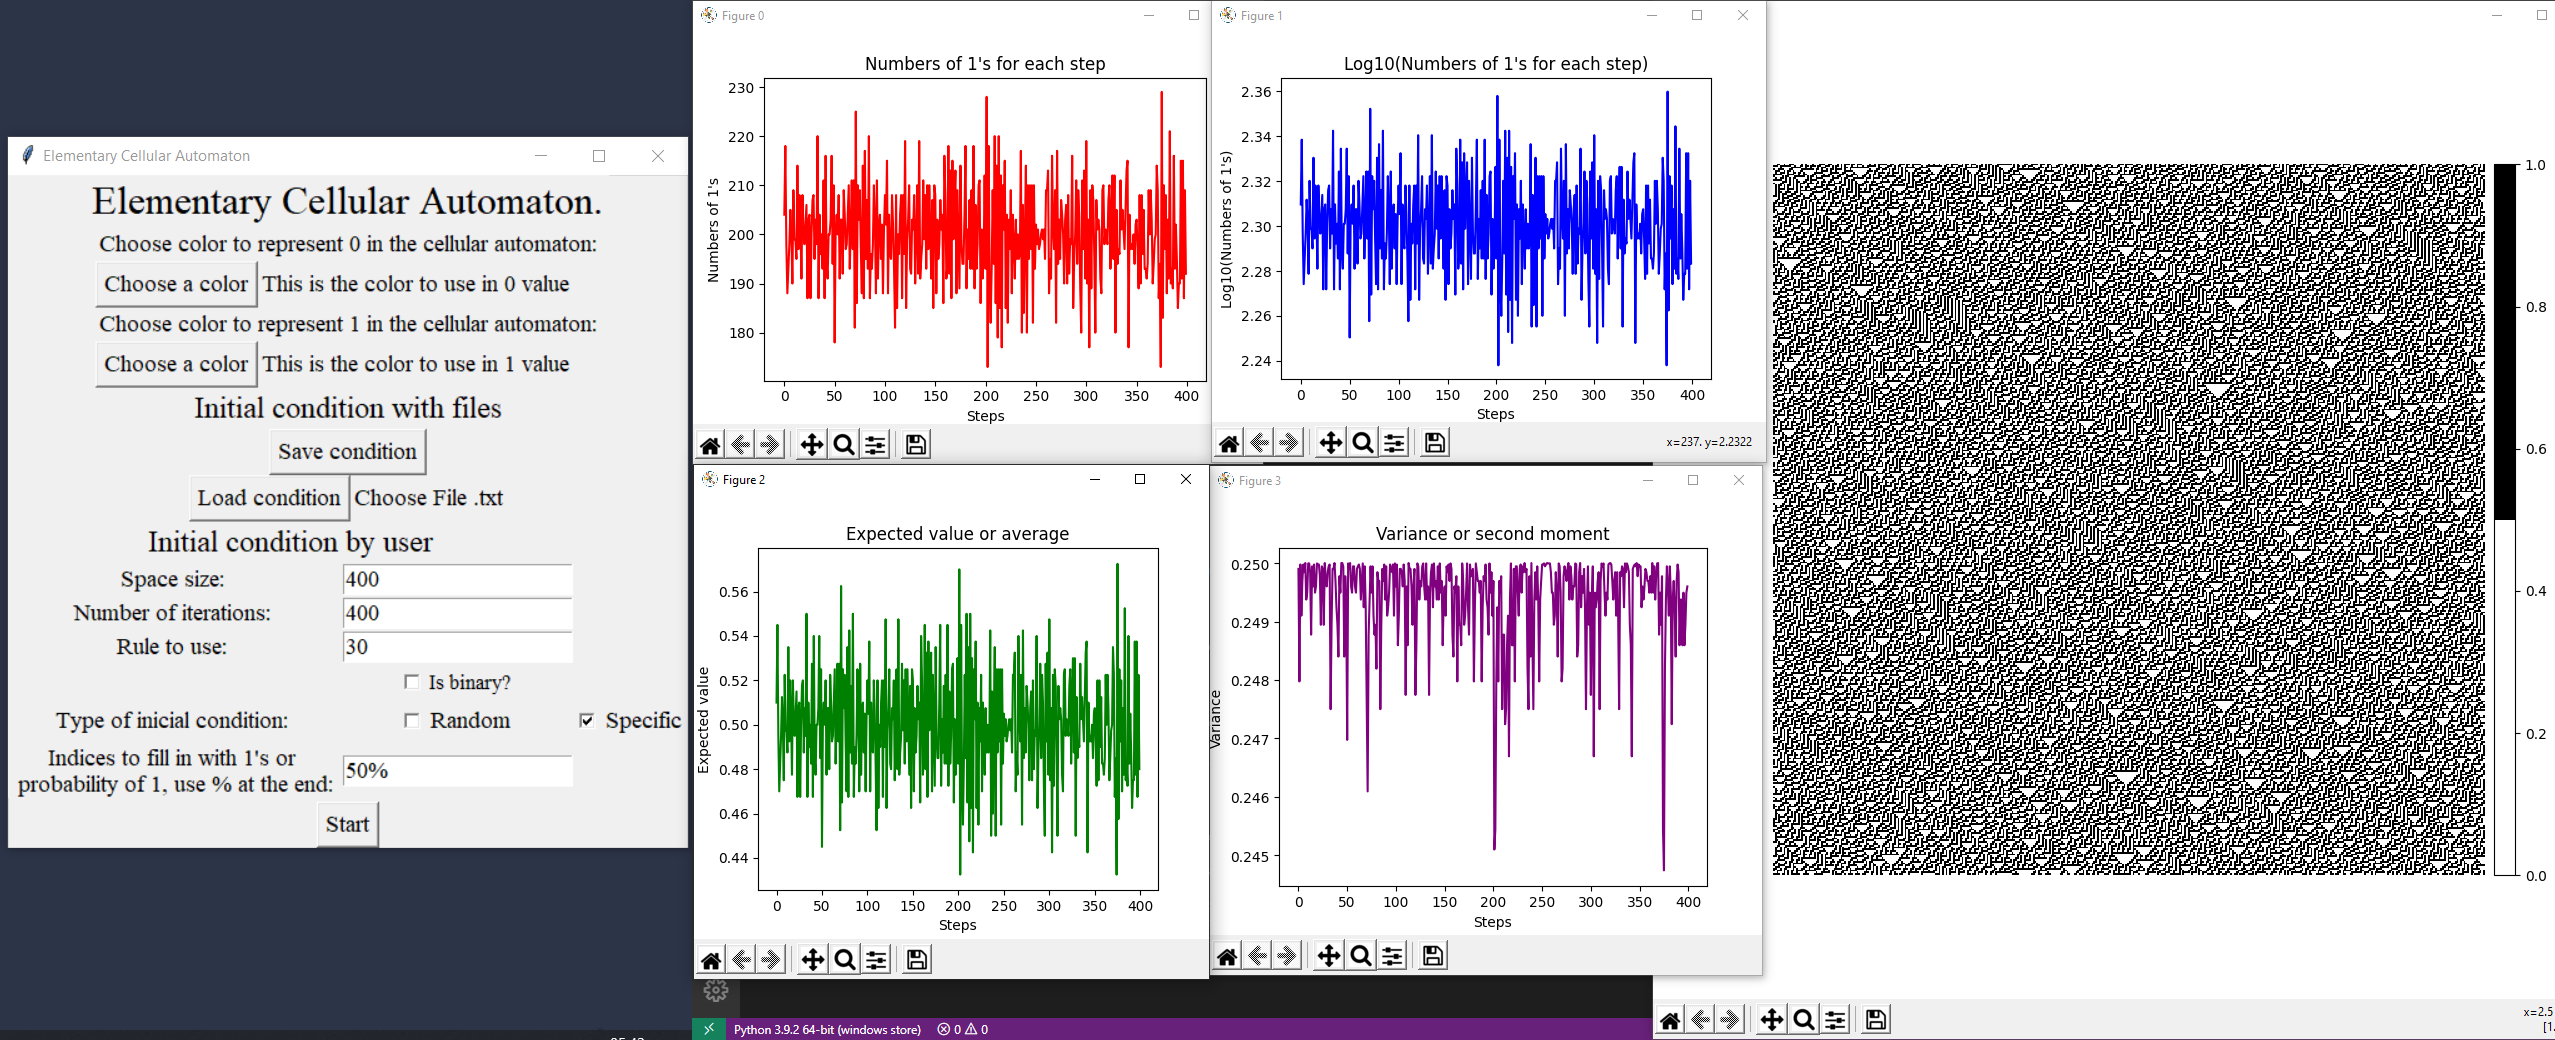
\includegraphics[scale=0.26]{resources/add8.png}
			\caption{ECA de 400 células por 400 iteraciones con 50\% de probabilidad de 1's, regla 30}								\label{fig:picture}
		\end{figure}
		\begin{figure}[H]
			\centering
			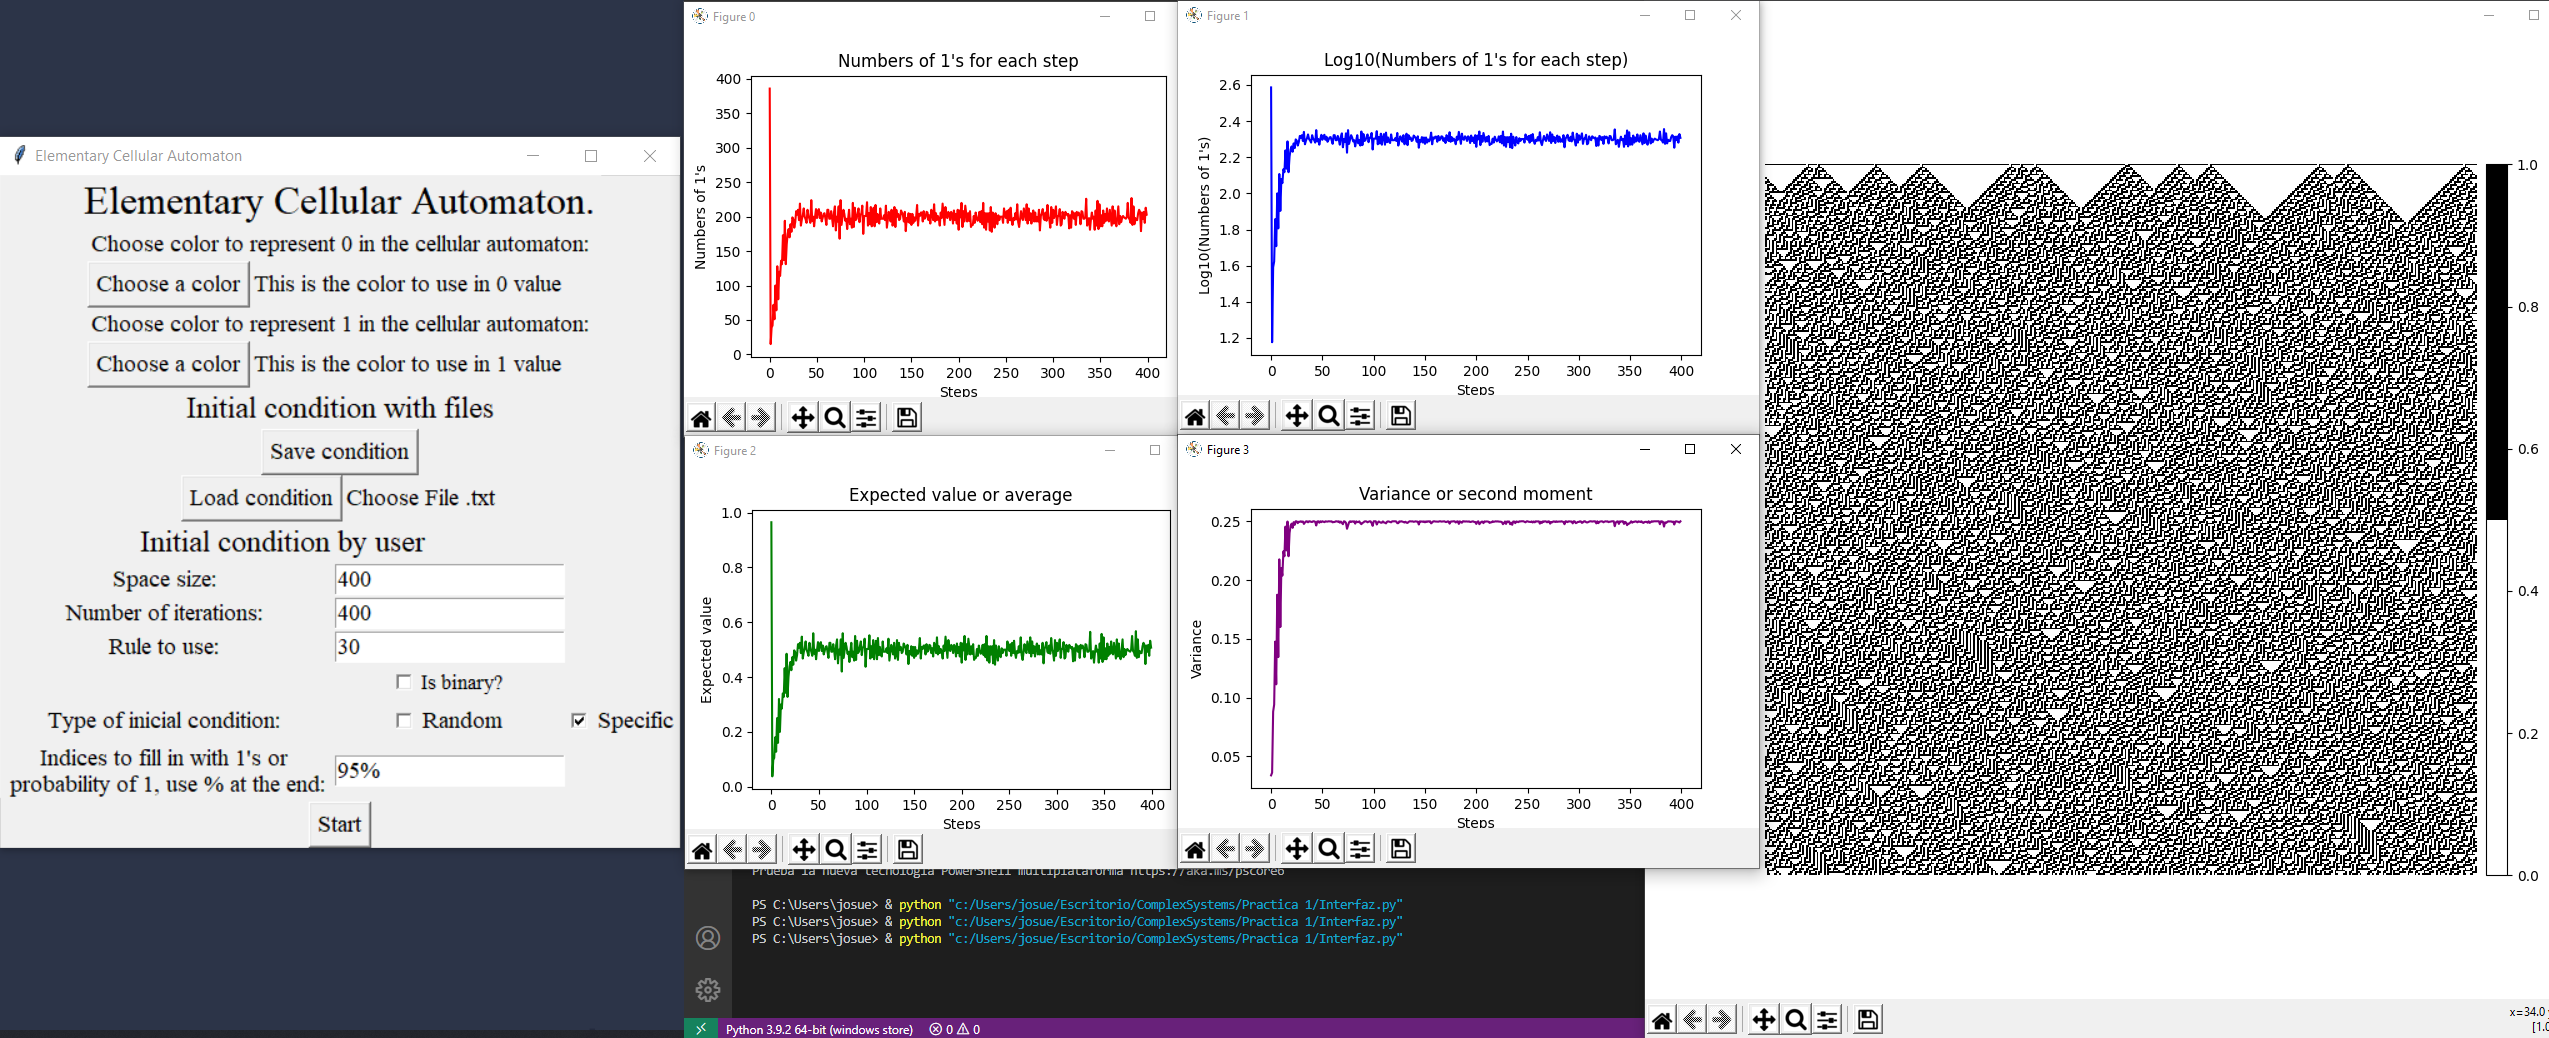
\includegraphics[scale=0.26]{resources/add9.png}
			\caption{ECA de 400 células por 400 iteraciones con 95\% de probabilidad de 1's, regla 30}								\label{fig:picture}
		\end{figure}
		Como vemos en las figuras 18 a la 20 esta regla nos recuerda el comportamiento de la regla anterior, en el sentido de que las figuras 18 y 20 son muy similares en su comportamiento el cual es como un crecimiento logarítmico, en cambio la figura 19 tiene un comportamiento caótico.\par
		Continuando, ahora veremos la regla 54.
		\begin{figure}[H]
			\centering
			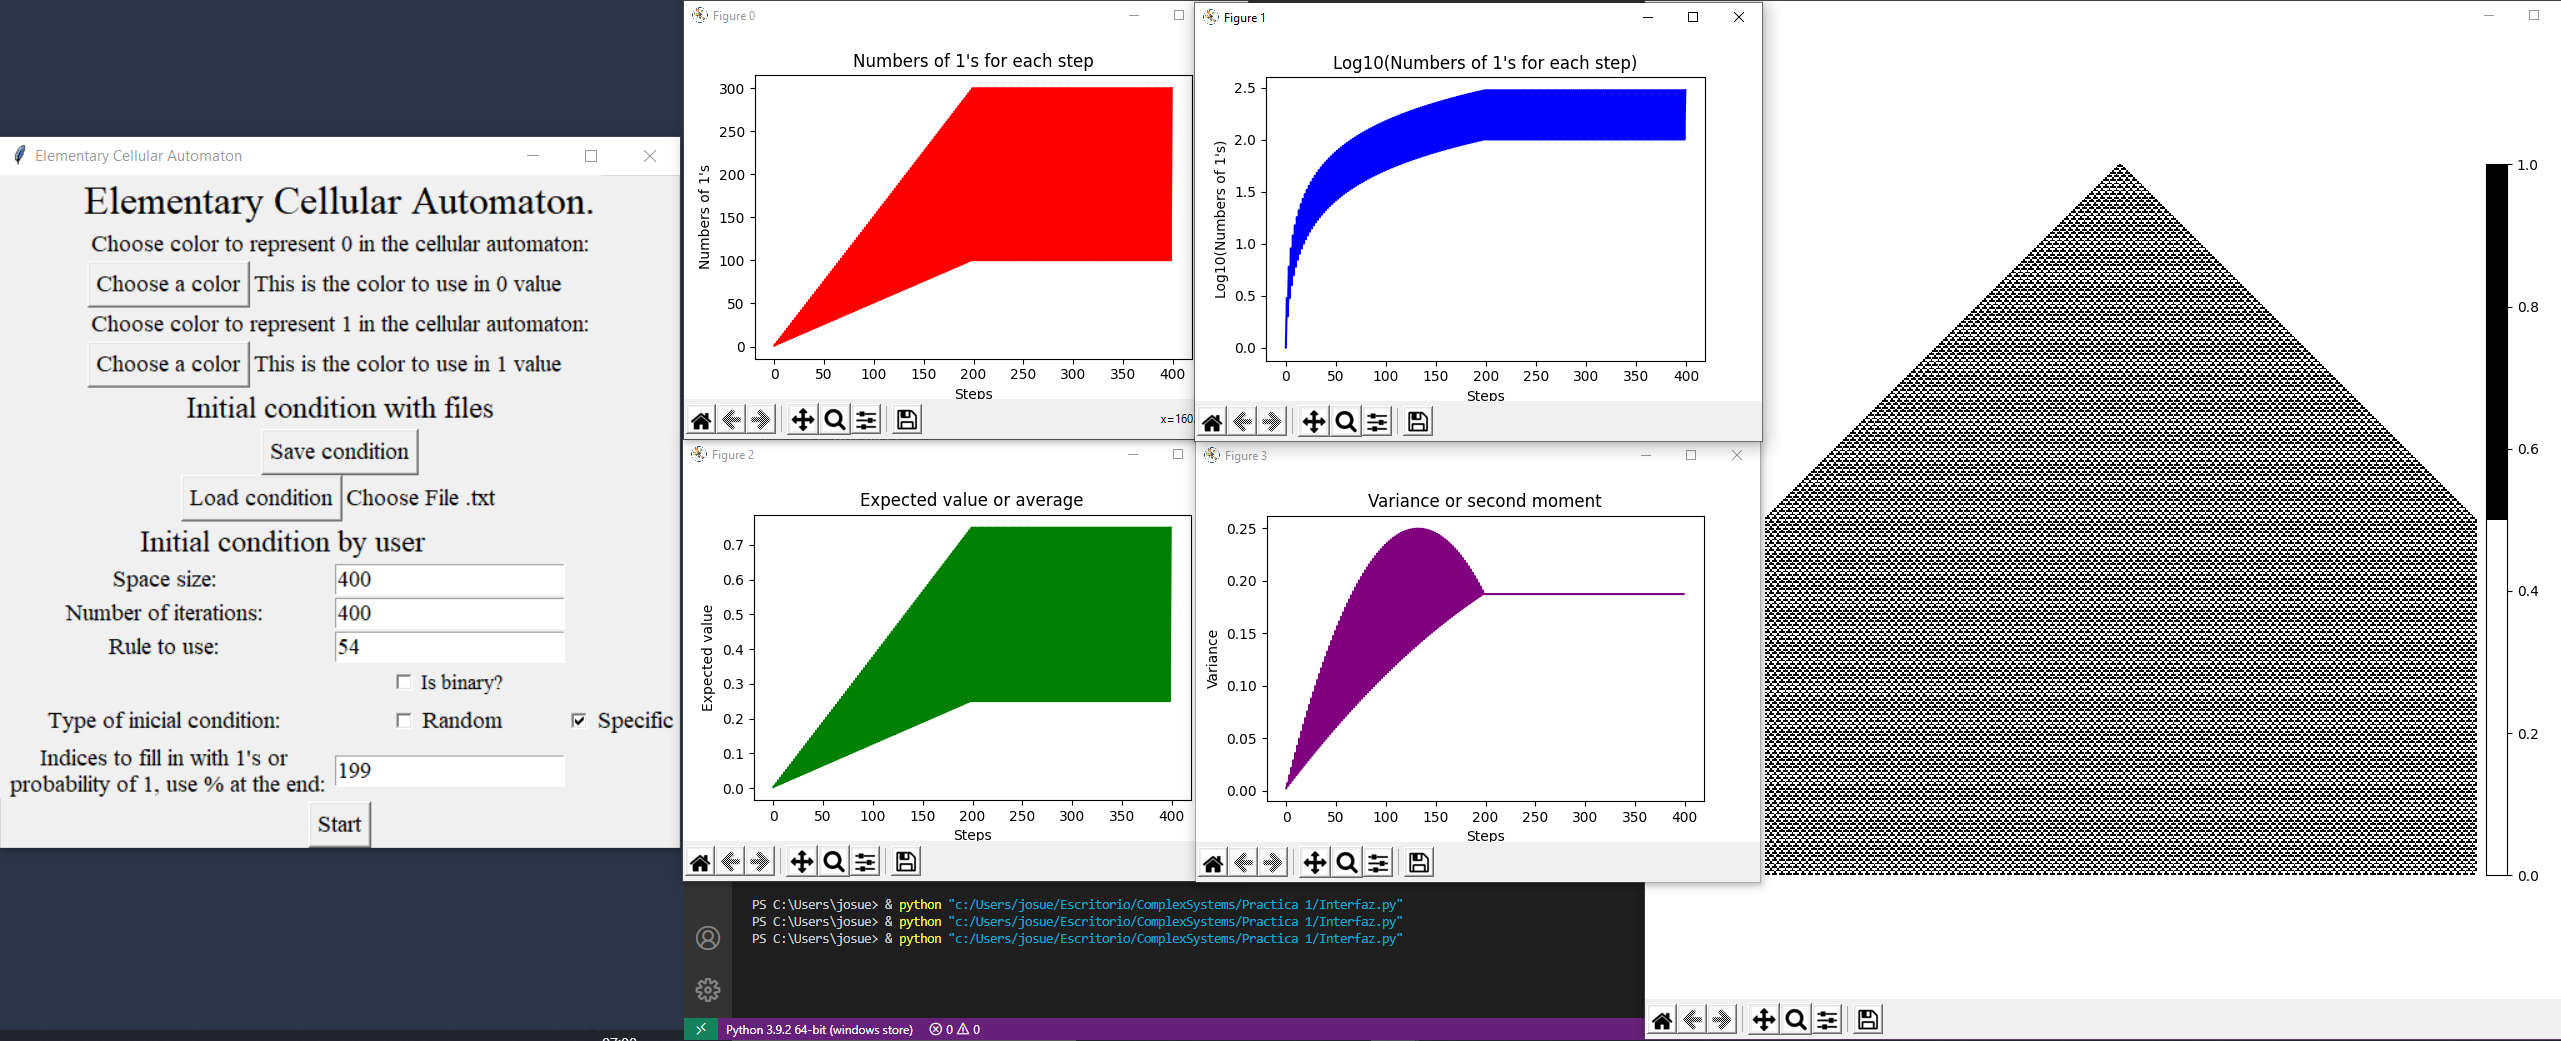
\includegraphics[scale=0.26]{resources/add10.png}
			\caption{ECA de 400 células por 400 iteraciones con una célula inicial central, regla 54}								\label{fig:picture}
		\end{figure}
		\begin{figure}[H]
			\centering
			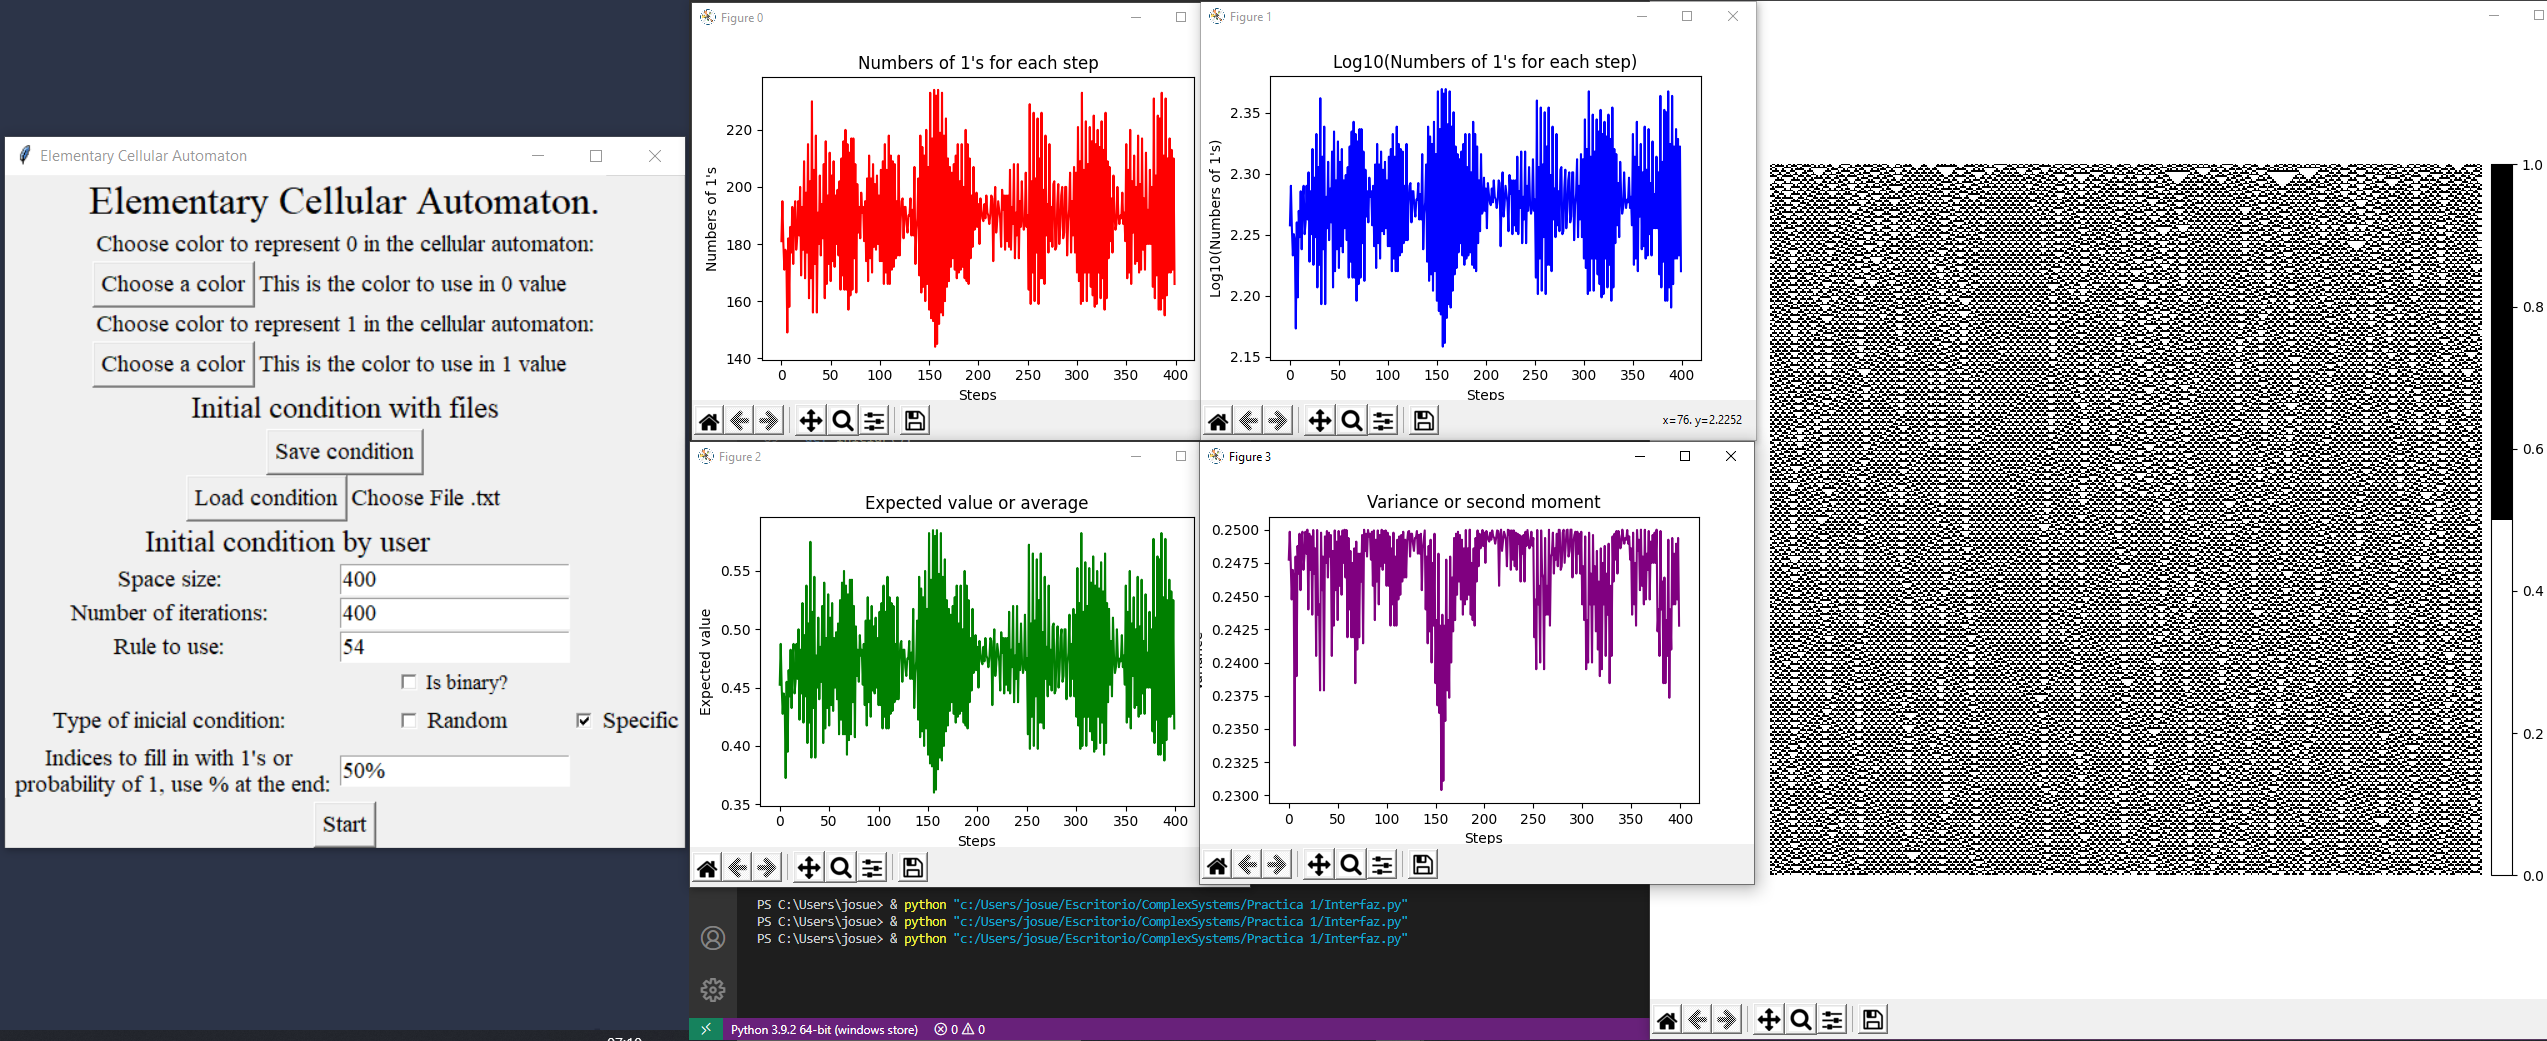
\includegraphics[scale=0.26]{resources/add11.png}
			\caption{ECA de 400 células por 400 iteraciones con 50\% de probabilidad de 1's, regla 54}								\label{fig:picture}
		\end{figure}
		\begin{figure}[H]
			\centering
			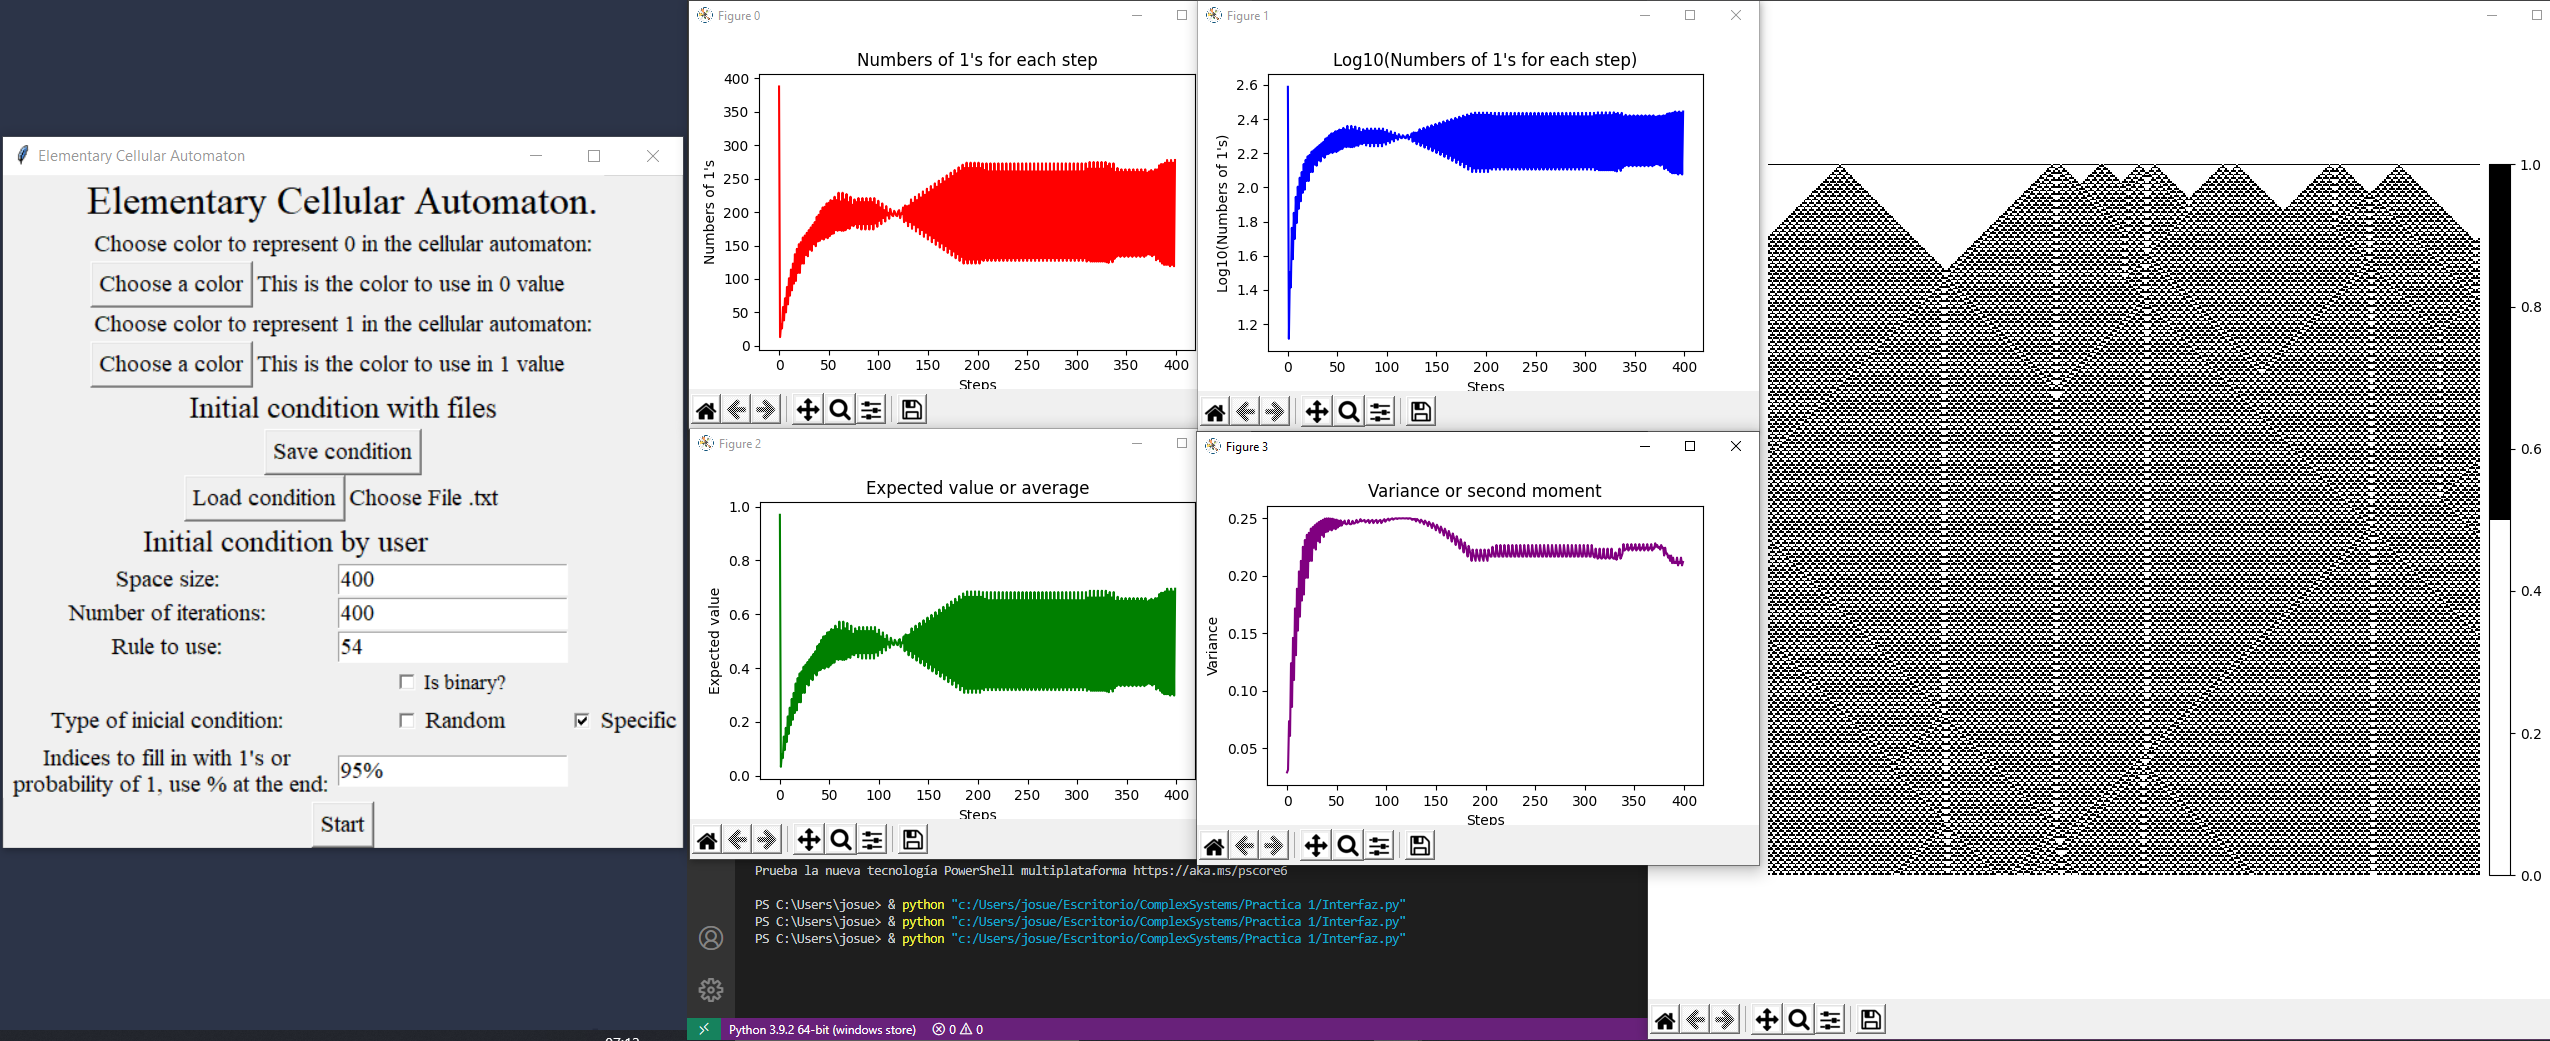
\includegraphics[scale=0.26]{resources/add12.png}
			\caption{ECA de 400 células por 400 iteraciones con 95\% de probabilidad de 1's, regla 54}								\label{fig:picture}
		\end{figure}
		Con esta regla si observamos un cambio en nuestras 3 pruebas que las 3 son diferentes entre si, pero, si observamos la figura 22 y la 23 encontramos una similitud un poco sutil en nuestro ECA y es que ambos generan lineas rectas que $"$dividen$"$ a nuestro ECA de formar vertical, caso contrario a la figura 21 que podríamos decir que esa división pasa a su forma horizontal\par 
		Pasando con la penúltima regla a probar la cual es la regla 110.
		\begin{figure}[H]
			\centering
			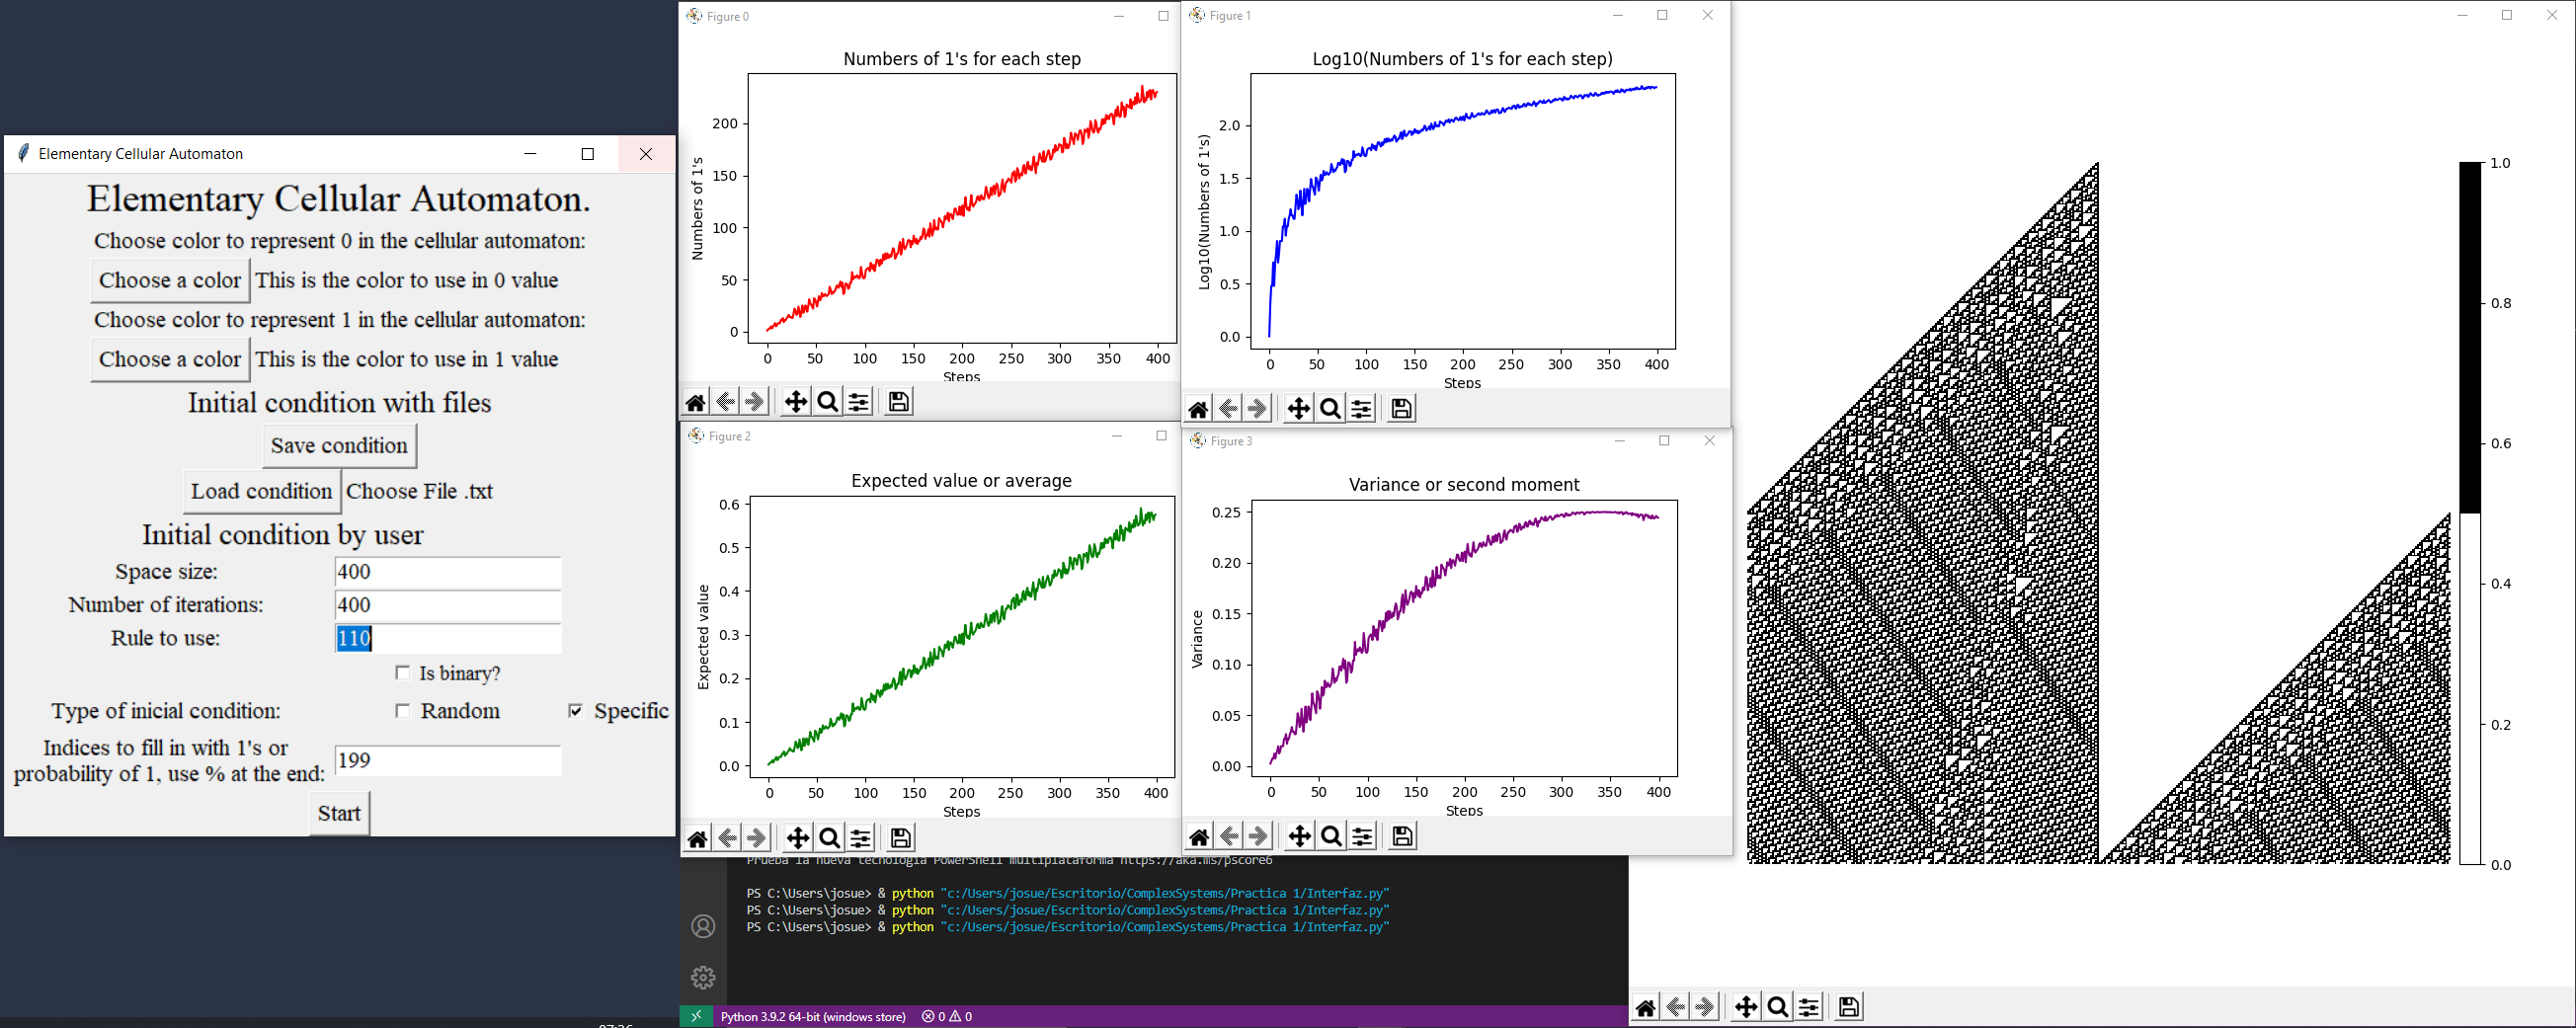
\includegraphics[scale=0.26]{resources/add13.png}
			\caption{ECA de 400 células por 400 iteraciones con una célula inicial central, regla 110}								\label{fig:picture}
		\end{figure}
		\begin{figure}[H]
			\centering
			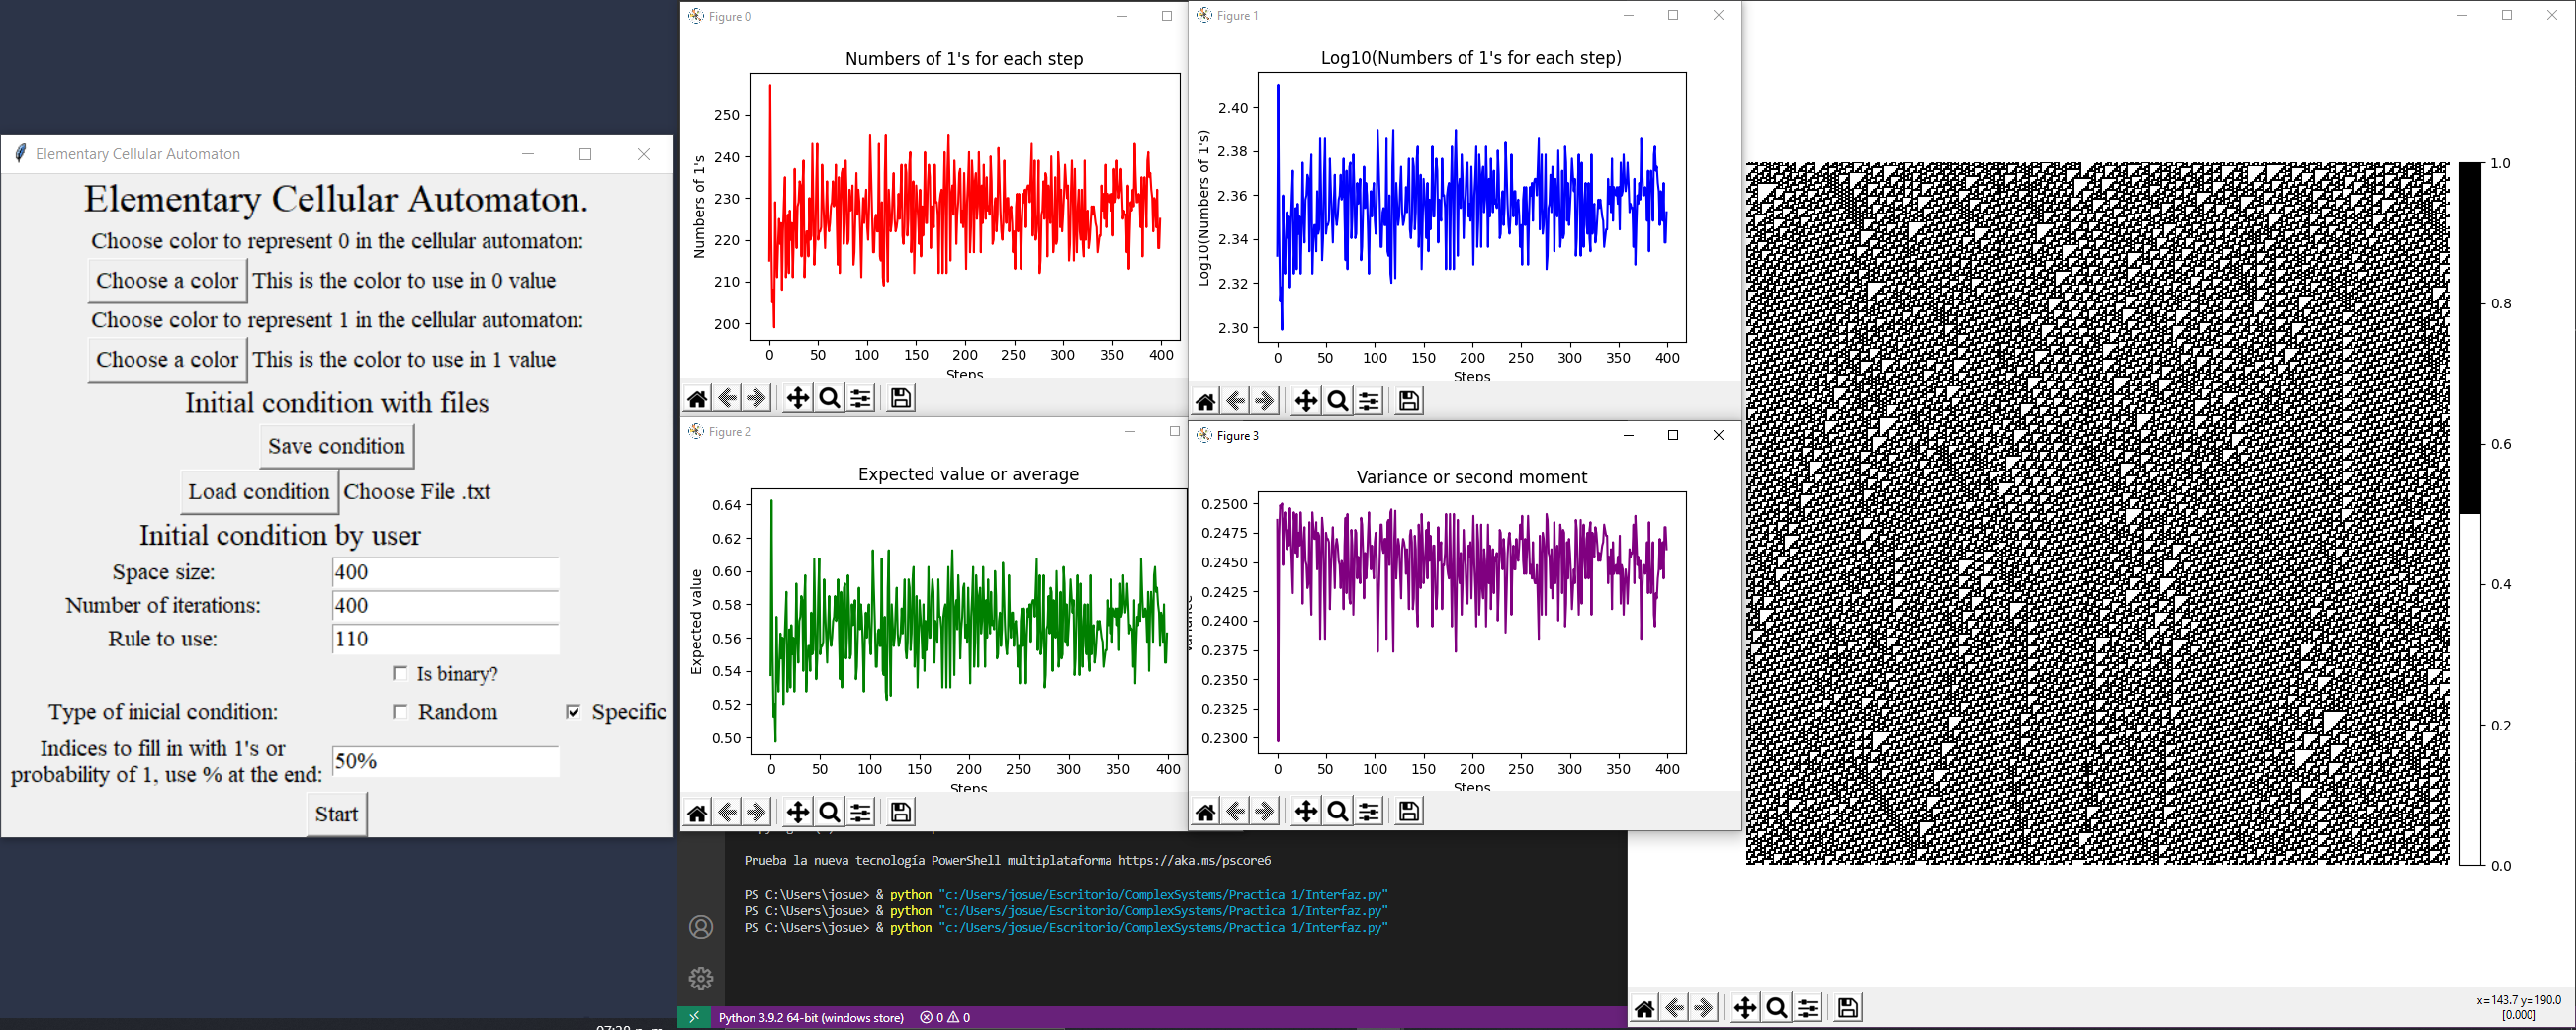
\includegraphics[scale=0.26]{resources/add14.png}
			\caption{ECA de 400 células por 400 iteraciones con 50\% de probabilidad de 1's, regla 110}								\label{fig:picture}
		\end{figure}
		\begin{figure}[H]
			\centering
			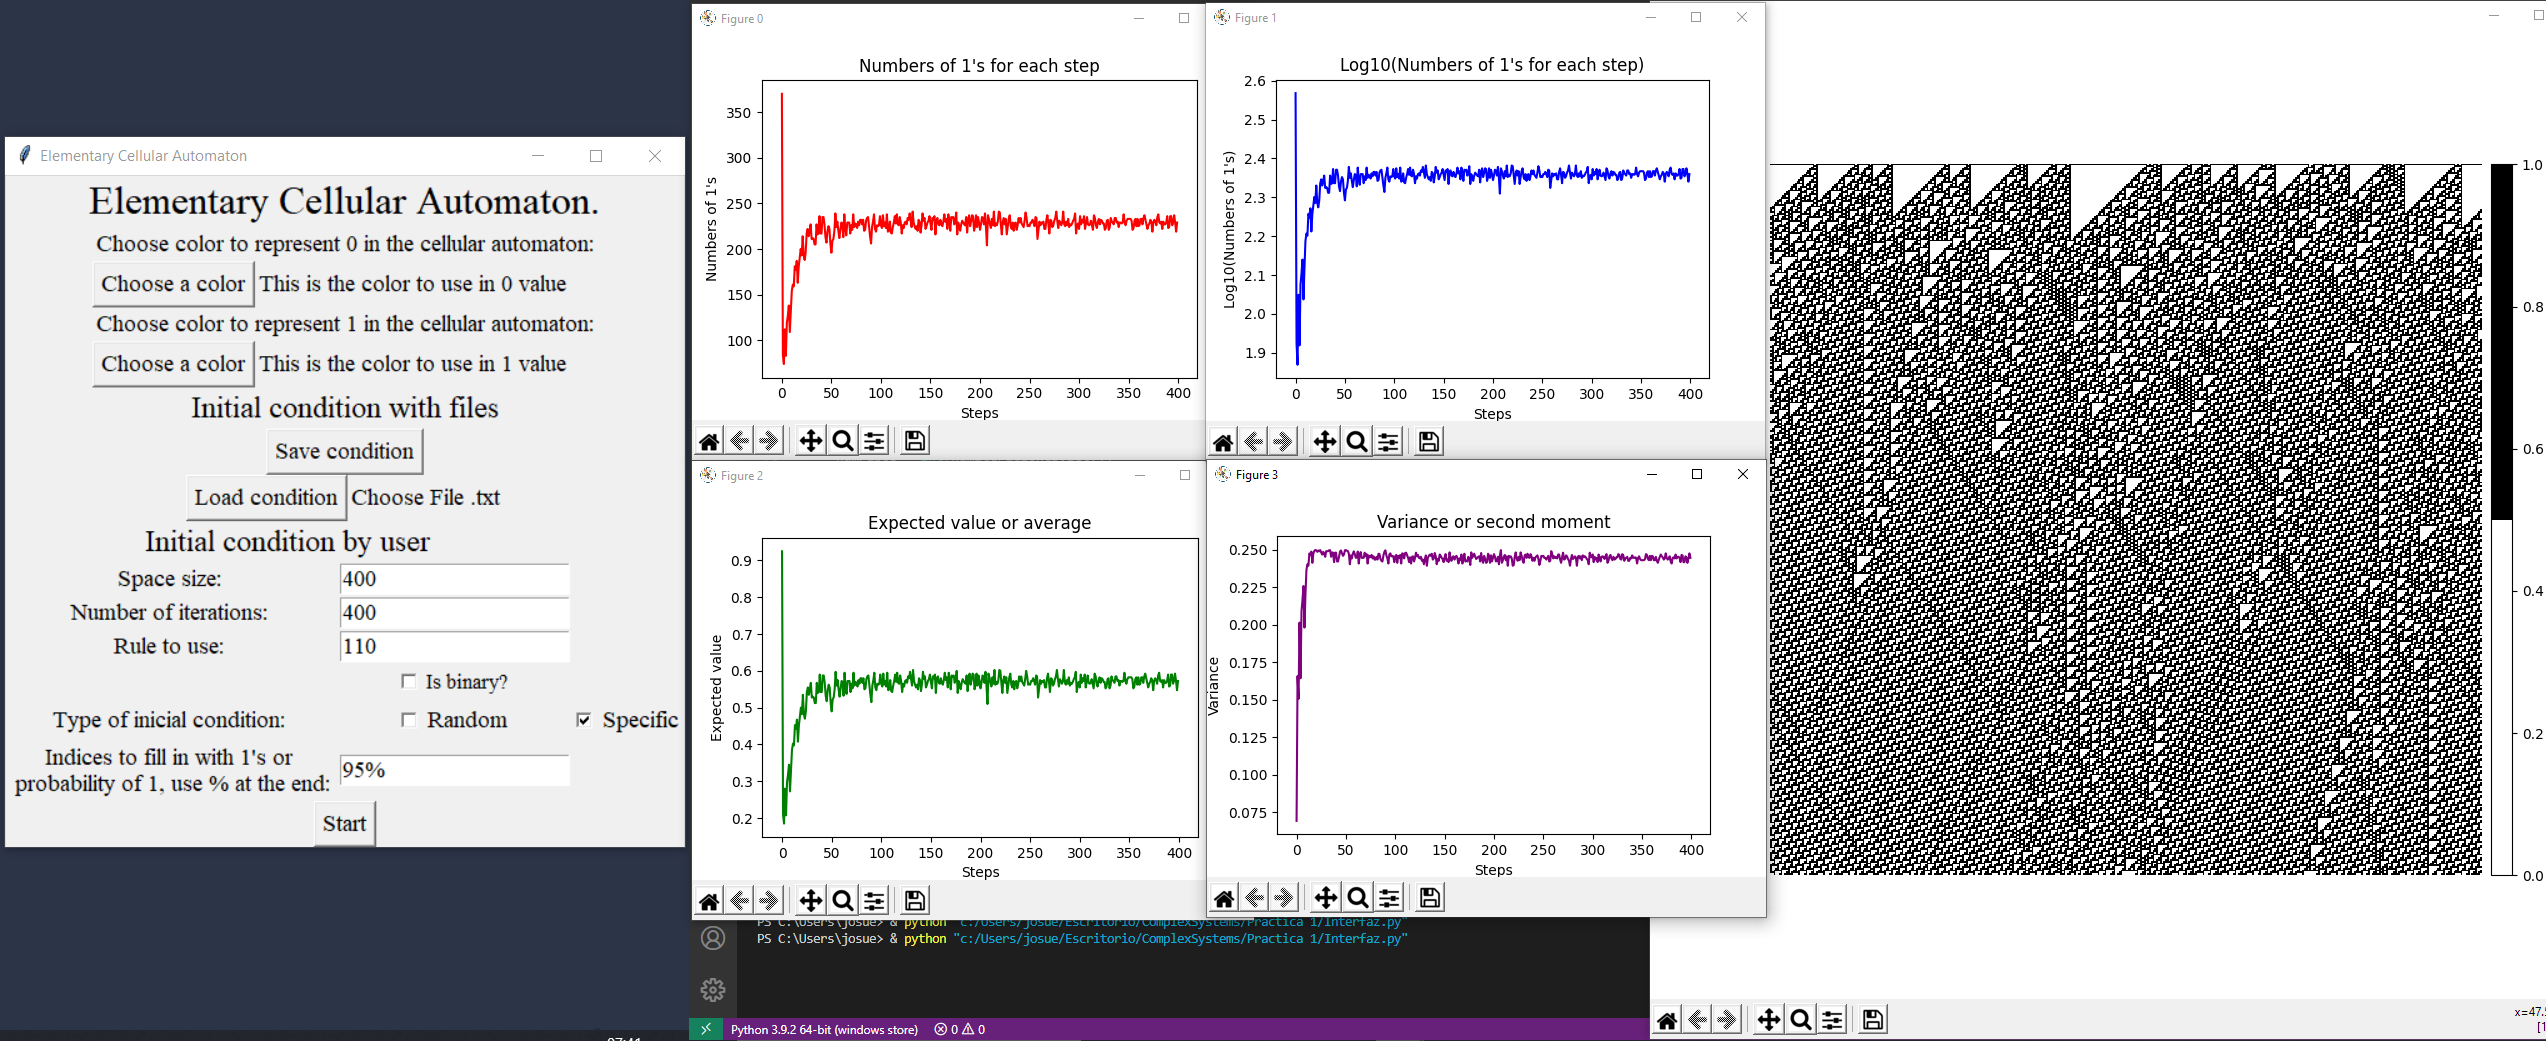
\includegraphics[scale=0.26]{resources/add15.png}
			\caption{ECA de 400 células por 400 iteraciones con 95\% de probabilidad de 1's, regla 110}								\label{fig:picture}
		\end{figure}
		Sin duda es la regla con un comportamiento muy interesante, en la figura 24 vemos un crecimiento lineal en los números de células con valor 1, caso contrario de las figuras 25 y 26 las cuales tienen un comportamiento diferente la cual nos recuerda al crecimiento logarítmico, pero, mencionar que la figura 25 no se visualiza tan claramente este comportamiento, de hecho pareciera que estuviéramos algún tipo de filtro en las gráficas de la figura 25 y así obtenemos las gráficas de la figura 26.\par
		Finalmente, tenemos la regla 126.
		\begin{figure}[H]
			\centering
			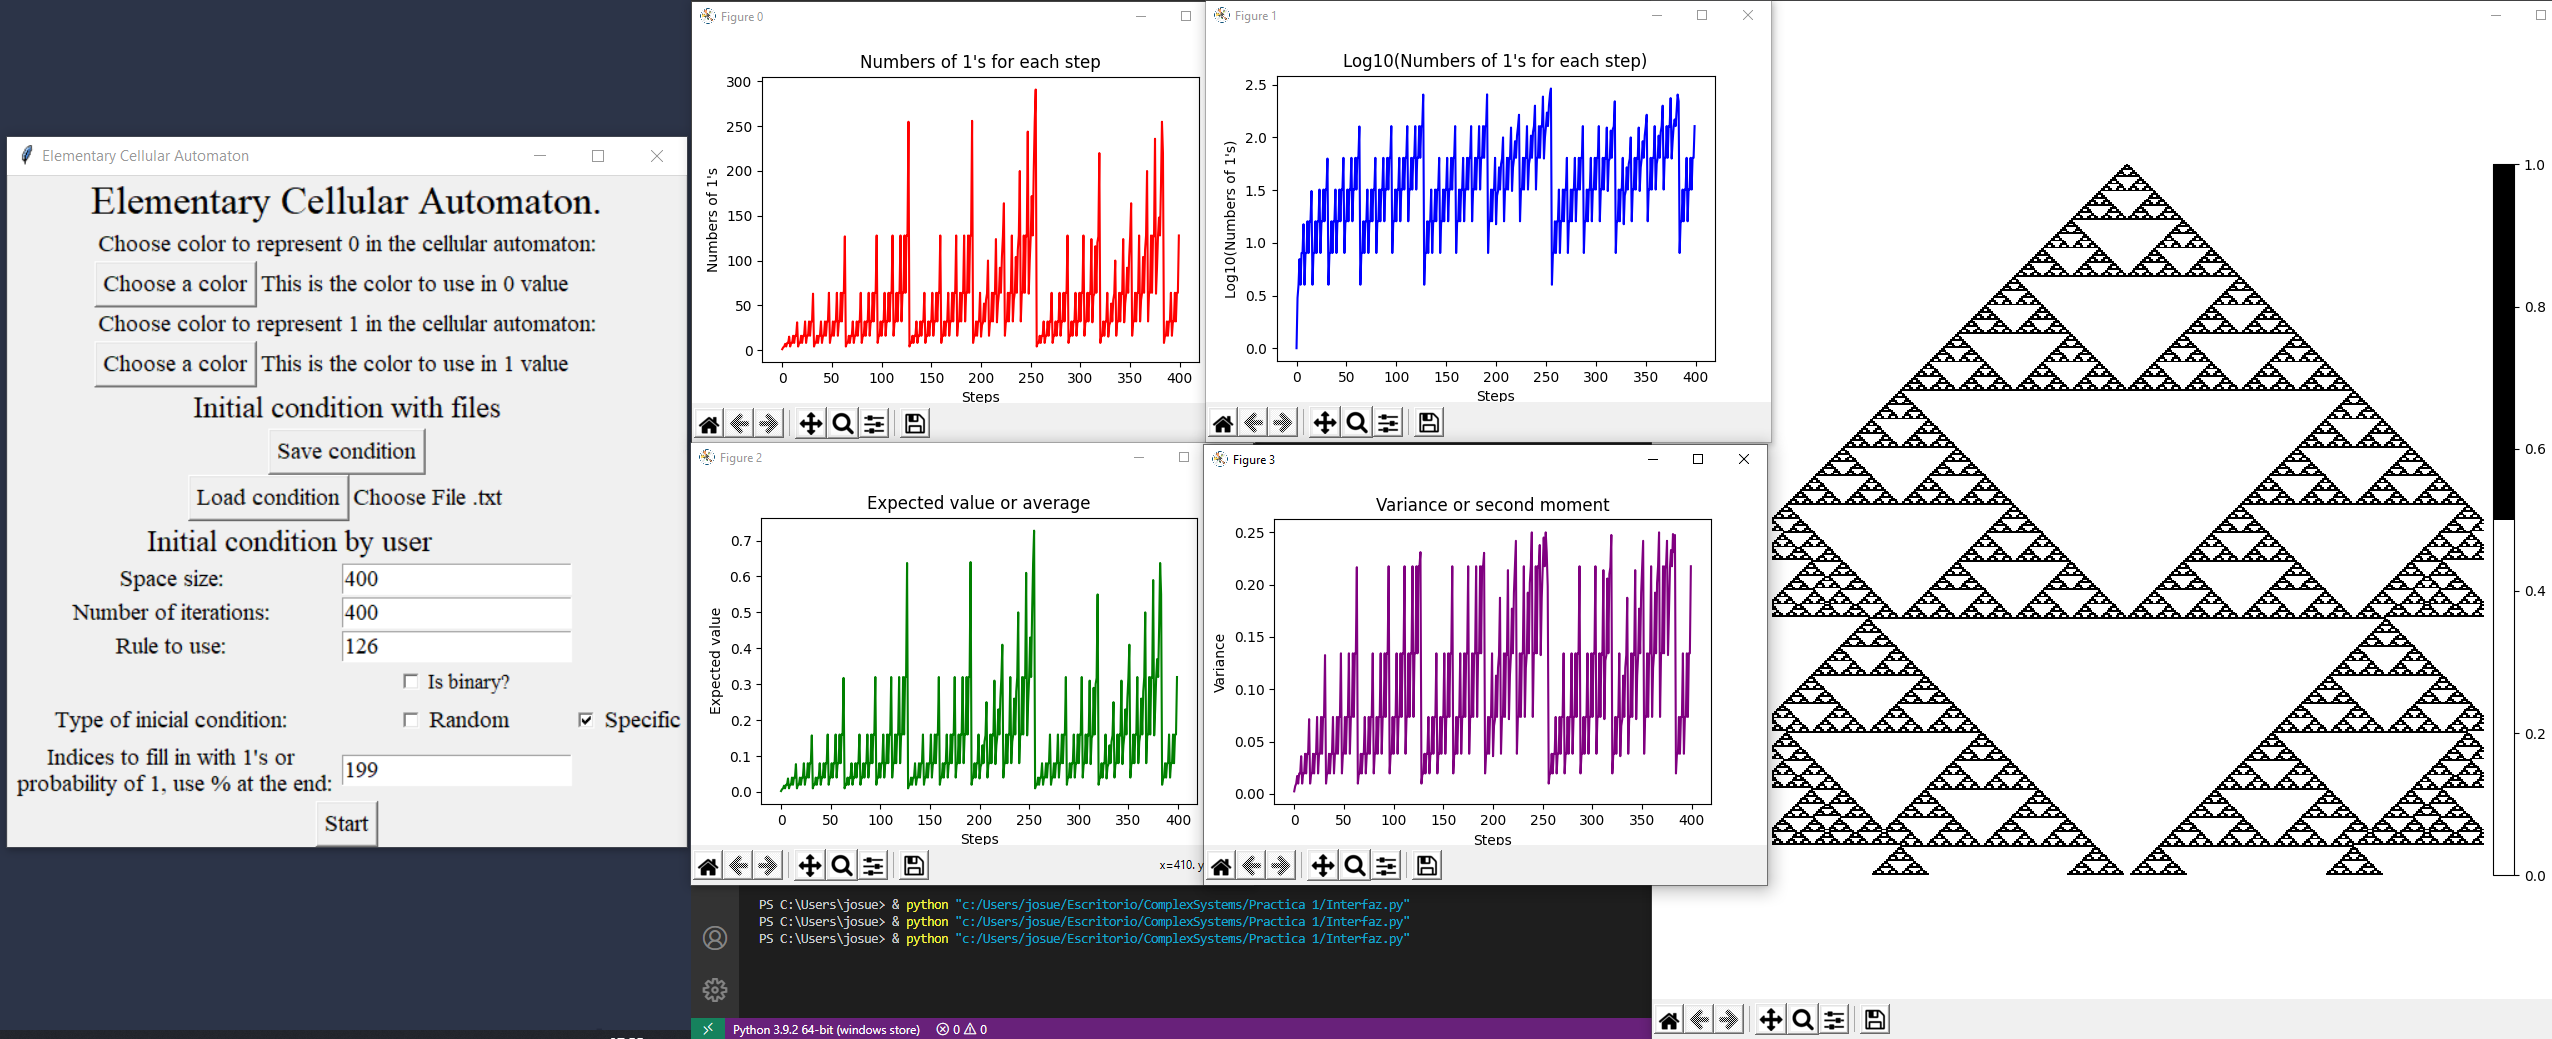
\includegraphics[scale=0.26]{resources/add16.png}
			\caption{ECA de 400 células por 400 iteraciones con una célula inicial central, regla 126}								\label{fig:picture}
		\end{figure}
		\begin{figure}[H]
			\centering
			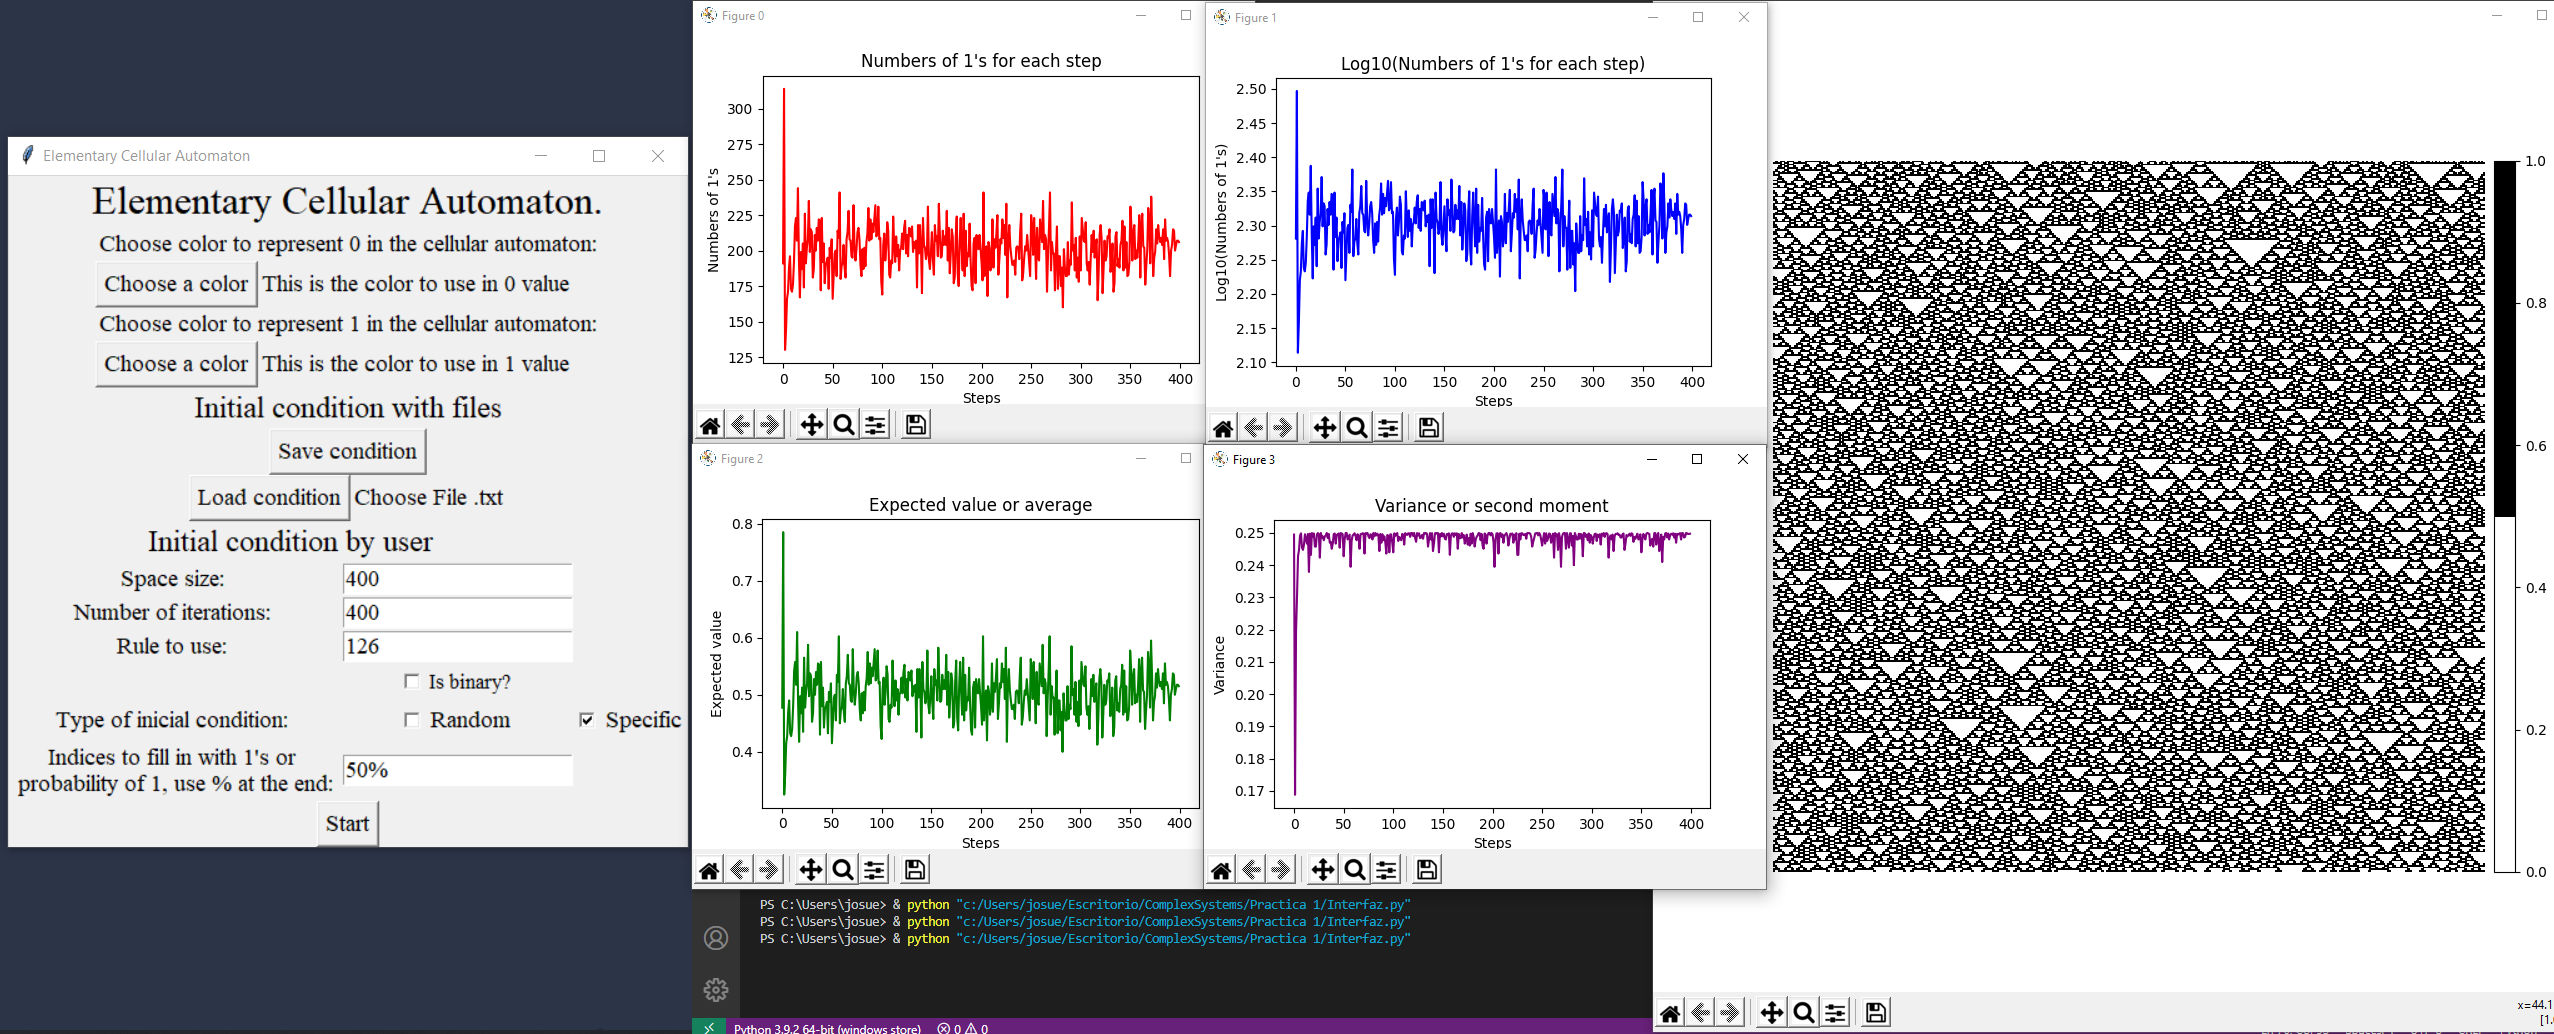
\includegraphics[scale=0.26]{resources/add17.png}
			\caption{ECA de 400 células por 400 iteraciones con 50\% de probabilidad de 1's, regla 126}								\label{fig:picture}
		\end{figure}
		\begin{figure}[H]
			\centering
			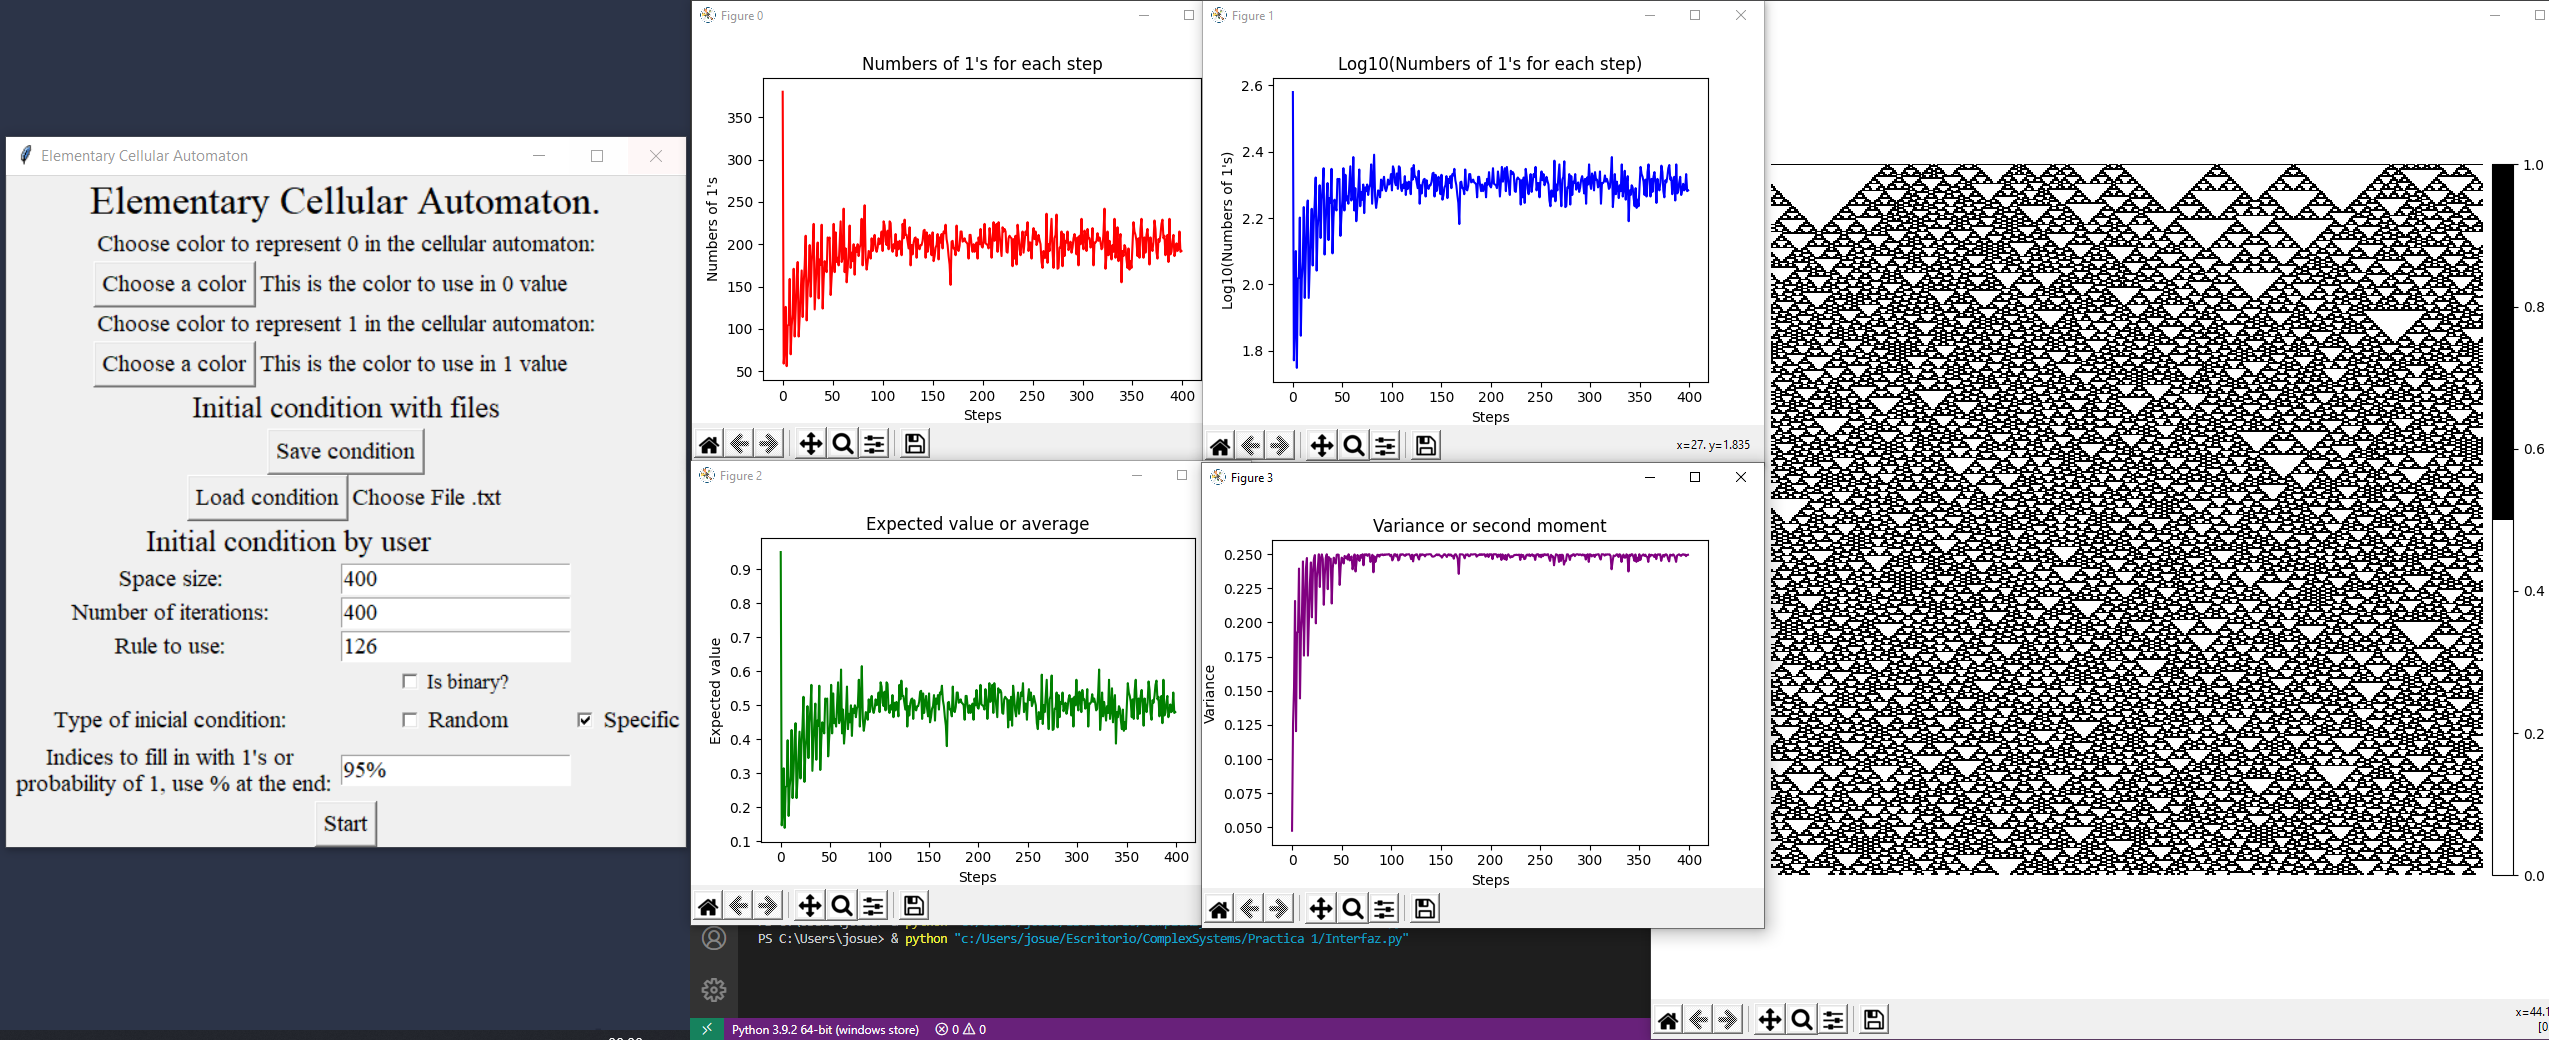
\includegraphics[scale=0.26]{resources/add18.png}
			\caption{ECA de 400 células por 400 iteraciones con 95\% de probabilidad de 1's, regla 126}								\label{fig:picture}
		\end{figure}
		En el caso de la regla 126 nos recuerda a la regla 22 y es que las imágenes resultantes son muy parecidas, sin embargo, en los casos del 50\% y 95\% vemos como ahora las gráficas son mas definidas en contraste a la regla 22 y que de hecho se parecen a gráficas anteriores en donde mencionamos que se nos recuerda a un crecimiento logarítmico.
		\subsection{Añadidos}
		Como añadidos al programa se agregaron 3 tipos de gráficas, las cuales son las siguientes:
		\begin{itemize}
    		\item Gráfica de logaritmo base 10 de la cantidad de células con valor 1 por cada iteración.
		    \item Gráfica del valor esperado o promedio.
		    \item Gráfica de la varianza o segundo momento.
		\end{itemize}\par		
 		La primera gráfica aplica el $\log$ a la cantidad de células con el valor 1 por cada iteración . Para la segunda gráfica se nos muestra el valor esperado para valores discretos el cual esta definido por la siguiente formula:   \[ \mu = E[x] = \sum_{x} x*f(x)\] En donde x toma los valores de 0 y nuestra f(x) es la probabilidad para que x sea 0 o 1, para sacar esa probabilidad solo se cuenta la cantidad de unos por iteración y se divide por el tamaño de nuestro autómata, si nos detenemos por un momento en la formula nos damos cuenta de que no es necesario tener $f(x=0)$ ya que se multiplicaría por un 0, por lo que nuestra formula para esa gráfica nos quedaría lo siguiente: \[ E[x] = \sum_{x} x*f(x) = 1*f(x=1) + 0*f(x=0) = f(x=1)\]	\[ E[x] = f(x=1)\]
 		Por lo que $E[x]$ tomaría el valor de la cantidad de números de 1's entre la longitud del autómata.\par
 		Finalmente para la gráfica de la varianza o segundo momento se usa la siguiente formula para el caso discreto. \[ \sigma^2 =  E[(x-\mu)^2]\] La cual puede ser reducida mediante desarrollo matemático quedando de la siguiente manera: \[ \sigma^2 =  E[(x-\mu)^2] = E[x^2-2x\mu+\mu^2]\]        \[ \sigma^2 = E[x^2]-E[2x\mu]+E[\mu^2]\]	\[ \sigma^2 = E[x^2]-2\mu E[x]+\mu^2\]						\[ \sigma^2 = E[x^2]-2\mu\mu+\mu^2\]	\[ \sigma^2 = E[x^2]-2\mu^2+\mu^2\] Finalmente tenemos que: 	\[ \sigma^2 = E[x^2]-\mu^2\]
 		Por lo que, retomando lo mencionado para el desarrollo de la gráfica 2 o la gráfica de nuestro promedio o valor esperado solo necesitamos el valor de $f(x=1)$, nuestra nuestra formula para la varianza y finalmente saber que $E[x^n] =  \sum_{x} x^n *f(x) $, así, sustituyendo valores obtendríamos lo siguiente sera: \[ \sigma^2 = (1^2*f(x=1)) - f(x=1)^2 = f(x=1) - f(x=1)^2 \] Finalmente la formula a usar para la varianza: \[ \sigma^2 = f(x=1) - f(x=1)^2 \]
 		Ahora hagamos una prueba, en la cual la regla a usar sera la regla 30, un tamaño de 1000 células con 1000 iteraciones, colores por defecto y asignación de células con valor 1 de manera aleatoria.
 		\begin{figure}[H]
			\centering
			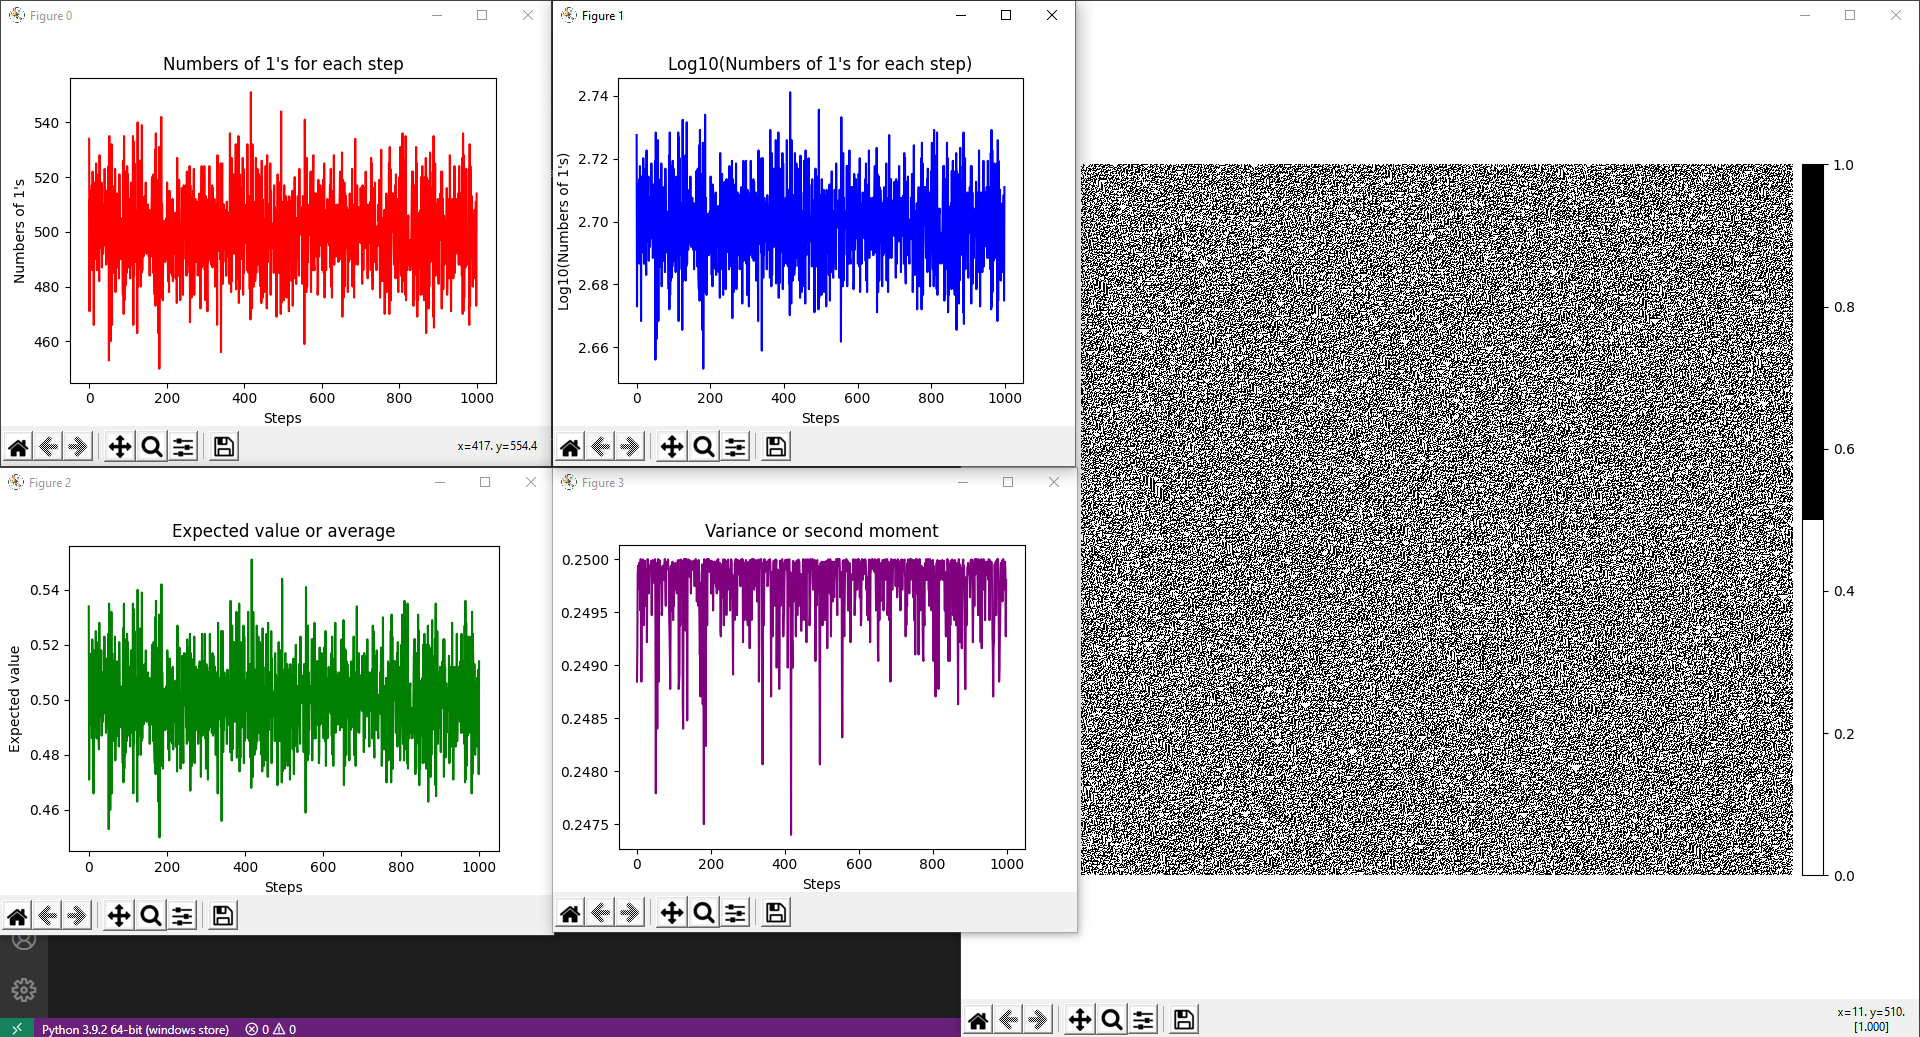
\includegraphics[scale=0.35]{resources/pruebaF1.png}
			\caption{ECA de 1000 células por 1000 iteraciones creado de forma aleatoria}\label{fig:picture}
		\end{figure}
		Como podemos observar tenemos 3 graficas que tienen una forma similar o casi iguales las cuales son la cantidad de 1's por iteración, $log$ de la cantidad de 1's y el valor esperado, esto es lógico ya que solo estamos cambiando la $"$escala$"$ de una misma representación, la única gráfica que difiere de las demás es la varianza y esto resulta, como dato adicional al momento de usar diferentes reglas el comportamiento de esta difiere e incluso en ocasiones llega a ser similar con las otras 3. Como nota adicional mencionar que a cada gráfica le podemos incrementar el tamaño de la gráfica para poder visualizar de una mejor visualización de los datos, lo anterior se realiza exactamente igual que a como se menciono unas hojas atrás.\par
		Adicionalmente a lo anterior, la barra de opciones que tiene cada gráfica nos permite realizar diferentes cosas que en seguida enlistaremos, para comodidad tomar como referencia la figura 12 y ver los iconos de izquierda a derecha.
		\begin{enumerate}
		  \item El icono de la casa nos permite reajustar la vista de nuestra gráfica a como lo era originalmente.
		  \item El icono de la flecha a la izquierda o derecha nos permite navegar entre las distintas vistas que hayamos realizado en una gráfica, es decir, si hicimos dos aumentos y queremos regresar al primero hacemos de la flecha hacia la izquierda y en caso de que estando en el primer aumento queremos regresar al segundo hacemos uso de la flecha a la derecha.
		  \item El icono que nos recuerda a una cruz nos permite mover la gráfica a voluntad, un ejemplo de uso seria que al hacer zoom en un área y querer mover ese mismo zoom en un área que tenemos a lado hacemos uso de esta función para poder mover nuestra gráfica.
		  \item El icono de la lupa como ya se ha mencionado nos permite aumentar el tamaño de cierta área en nuestra gráfica.
		  \item El icono que nos recuerda a configuración no recomiendo usarlo ya que cambia la configuración inicial de nuestra gráfica y en ocasiones nos arruina el como se ve la gráfica
		  \item El ultimo icono, que es el icono de disquete nos permite, como es incluso lógico, guardar la gráfica como una imagen con varias extensiones a elegir, esto nos permite poder guardar resultados como una imagen para el posterior uso.
		\end{enumerate}
		\begin{figure}[H]
			\centering
			
\includegraphics[scale=1]{resources/barra.png}
			\caption{Barra de opciones}\label{fig:picture}
		\end{figure}
		\newpage
		\subsection{Código}
	A continuación se anexa el código generado para la creación de este primer programa. Primero
tenemos la parte de la interfaz de nuestro programa que se crea con el siguiente código.\lstinputlisting[language=Python]{../Interfaz.py}
\par
	Por ultimo tenemos el código que nos proporciona la parte lógica del programa y que ademas es el encargado de hacer las gráficas, este código es el cerebro de nuestro programa.
	\lstinputlisting[language=Python]{../Logica.py}
	\section{Conclusiones}
	Esta programa es bastante interesante, ya que es increíble ver al cambiar los valores de las células de nuestra iteración cero cambia por mucho el comportamiento de nuestro ECA que se podria pensar que no es tan significativo pero eso es un pensamiento errado ya que vemos 	que cambia demasiado, podríamos llegar a decir que una célula de mas o de menos provoca un caos en nuestro ECA y por tanto un ECA diferente cada vez que cambiemos nuestra iteración inicial. Finalmente solo me queda comentar que al haber ya probado diferentes reglas con la misma iteración inicial el resultado es muy diferente con cada regla.
	\begin{thebibliography}{1}
 \bibitem[label1]{cite_key1} Weisstein, E., 2021. Elementary Cellular Automaton - from Wolfram MathWorld. [online] Mathworld.wolfram.com. Available at: https://mathworld.wolfram.com/ElementaryCellularAutomaton.html [Accessed 15 March 2021].	
 \bibitem[label2]{cite_key2} Lees, E., 2020. Elementary Cellular Automata · Matplotblog. [online] Matplotlib.org. Available at: https://matplotlib.org/matplotblog/posts/elementary-cellular-automata/ [Accessed 15 March 2021].
  \bibitem[label3]{cite_key3} Caparrini, F., 2016. Autómatas Celulares - Fernando Sancho Caparrini. [online] Cs.us.es. Available at: \url{http://www.cs.us.es/~fsancho/?e=66} [Accessed 15 March 2021].
\end{thebibliography}

\end{document}